\chapter{Data Analysis}
\label{chap_ana}
%\section{Analysis Overview}
%\label{sec_4_overview}
The main aim of this analysis is to extract $J/\psi$ spectra at mid-rapidity region in p-Pb collisions.  
The analysis is performed using the minimum bias data of p-Pb collisions at $\sqrt{s_{NN}} =$ 5.02 TeV collected during LHC Run1 in 2013 winter.
$J/\psi$ measurements have been performed in ALICE central barrel using dielectron (electron-positron pair) decay channels. 
In this analysis, ITS and TPC are the main devices for the vertexing,  track reconstruction, and electron identification.
\begin{table}[!h]
\begin{center}
	\begin{tabular}{cccc} \hline
		$J/\psi$ Mass (GeV/$c$^{2})    & Decay Mode & Branching Ratio (\%) & Rapidity Acceptance \\ \hline
 		3.096                           & $e^{+}e^{-}$   &  5.96  $\pm$ 0.06                         & -1.37 $<$ $y$ $<$ 0.43 \\ \hline
	\end{tabular}
\end{center}
	\caption{General information of the $J/\psi$ measurements in the ALICE central barrel in p-Pb collisions at $\sqrt{s_{NN}}~=$~5.02 TeV}
\end{table}

The invariant cross section of $J/\psi$ production is calculated as following,  
\begin{equation}
  \cfrac{1}{2\pi p_{T}}\cfrac{d^{2}\sigma_{J/\psi}}{dp_{T}dy} =  \cfrac{1}{2\pi p_{T}}\cfrac{1}{BR(J/\psi\rightarrow e^{+}e^{-})} \times \cfrac{N_{J/\psi ,raw}}{\int{L}dt \times \epsilon \times \Delta y \Delta p_{T}}
\end{equation}
where $N_{J/\psi ,raw}$ is the number of reconstructed $J/\psi$ and $\epsilon$ is the detection efficiency of $J/\psi$. 
$\Delta p_{T}$ and $\Delta y$ are bin width of $p_{T}$ and rapidity $y$. 
$\int{L}dt$ is the integrated luminosity of the analyzed data.

Comparison of the $J/\psi$ production in p-Pb collisions and pp collisions is crucial to understand nuclear matter effects. 
The nuclear matter effects are quantified by the nuclear modification factor ($R_{\rm{pPb}}$) defined as, 
\begin{equation}
  R_{\rm{pPb}} = \cfrac{Y_{\rm{pPb}}}{\langle N_{coll}\rangle Y_{\rm{pp}}}
\end{equation}
where $\langle N_{coll}\rangle$ is the average number of binary nucleon-nucleon collisions in p-Pb collisions and $Y_{\rm{pPb}}$ and $Y_{\rm{pp}}$ are the yields in p-Pb and pp collisions, respectively.
If there is no effects of nuclei, this value should be unity. 
On the other hand, the deviation from unity indicates the presence of nuclear matter effects.

$R_{\rm{pPb}}$ is calculated with the following equation in this analysis, 
\begin{equation}
\label{eq_4_rppb}
  R_{\rm{pPb}} (p_{\rm{T}}) = \cfrac{ \cfrac{ dY_{J/\psi , \rm{pPb}} }{ dp_{\rm{T}}dy } }{<T_{\rm{pPb}}>\times \cfrac{\sigma_{J/\psi, \rm{pp}}}{dp_{\rm{T}}dy}}
\end{equation}
where $Y_{J/\psi ,\rm{ pPb}}$ is the invariant yield of $J/\psi$ in p-Pb collisions. 
$T_{\rm{pPb}}$ is called "Nuclear Thickness Function'' expressed as, 
\begin{equation}
  T_{\rm{p}A}(b) = \int{dz \rho_{A}(b,z)} = \cfrac{\langle N_{coll}\rangle }{\sigma_{\rm{pp}}}
\end{equation}
 where $b$ is the impact parameter of p-Pb collisions and $\rho_{A}(b, z)$ is the nuclear density with mass number A.  
It is simply understood as the number of nucleons in the region where incident proton pass through a nuclei. 
It is normalized to satisfy the integral of the transverse plane $\int{T_{pA}} =$ A.

In minimum bias p-Pb collisions, $\langle T_{\rm{pPb}}\rangle =$ 0.0983 $\pm$ 0.0035 $\rm{mb}^{-1}$ is given by the Glauber model calculation~\cite{bib_tppb}.
The uncertainties of $\sigma_{\rm{pPb}}$ and $\langle N_{coll}\rangle$ can be canceled partially by calculating ${T_{\rm{p}A}}$.
%\begin{table}
  %\begin{tabular}{cc} \\ \hline
   % 
  %\end{tabular}
  %\caption{ }
%\end{table}

Following analysis steps are applied to calculate the invariant cross-section of $J/\psi$ in p-Pb collisions.
\begin{description}
  \item[1. Event selection and luminosity determination]
  \item[2. electron identification ]\mbox{}\\
    After the event selection, electrons are reconstructed by ITS and TPC and identified by the energy deposition in the TPC. 
  \item[3. Pair analysis based in invariant mass analysis ]\mbox{} \\
    After electrons and positrons are identified, invariant mass is calculated for all combination of pairs as follows:
    \begin{equation}
      m_{ee} = \sqrt{(E_{e^{+}}+E_{e^{-}})^{2}-(\vec{p_{e^{+}}} + \vec{p_{e^{-}}})^{2}}
    \end{equation}
    where $E_{e^{+}}=\sqrt{m_{e}^{2}+|\vec{p_{e^{+}}}|^{2}}$ and $E_{e^{+}}=\sqrt{m_{e}^{2}+|\vec{p_{e^{-}}}|^{2}}$ are energy calculated by the electron mass $m_{e}$ and reconstructed momentum and $\vec{p_{e^{+}}}$ and $\vec{p_{e^{-}}}$ are momentum of electrons and positrons, respectively.
  \item[4. Subtraction of background pairs from unlike-sign pairs]\mbox{} \\   
    In order to extract the number of reconstructed J/$\psi$ signals, background subtraction is needed. 
    The main source of the background is combinatorial pairs from totally uncorrelated electron-positron pairs. 
    In order to evaluate the combinatorial pairs, the event mixing technique is adopted.  
  \item[5. Acceptance and efficiency corrections.]\mbox{}\\
    To calculate the invariant yield, acceptance and efficiency corrections are extracted by using Monte-Carlo (MC) simulations.
\end{description}

In this chapter, the event selection is discussed first in Section.~\ref{sec_4_eventselection}.
Section~\ref{sec_4_trackrec} and \ref{sec_4_eid} describes how to reconstruct and select electron samples.  
Raw signal extraction of $J/\psi$ is discussed in Section.~\ref{sec_4_signalextraction}. 
Acceptance and efficiency correction is explained in Section.\ref{sec_4_correction}. 
%And then, the extraction of invariant yield is shown in this section.
The extraction of pp reference is also discussed in Section.~\ref{sec_4_ppref}.
%The calculation of the scaling factor is described in Section.\ref{sec_4_thickfunc}

\section{Event Selection}
\label{sec_4_eventselection}
\subsection{Minimum Bias Event Selection}
Minimum bias events are triggered using information of V0, T0 and SPD.
In this analysis, the criteria of the minimum bias trigger is coincidence of both hits in V0A and V0C.
In this condition, the trigger efficiency of the minimum bias events is 96.4\%. 
To reduce fake events caused by beam-gas and beam-halo collisions, the timing information of V0 and T0 are used. 

%should be discussed about pile-up?
%The $\mu$ of pile-up events for MB is about .
%Pile-up events are found by the primary vertex reconstruction using SPD. 
%The events which has at least 2 candidates of the primary vertex and fulfill the following requirements are rejected. 
%Primary vertex which is thought as the collision vertex is reconstructed by the hit on SPD detectors.
%It is determined as the 3-D center points of selected tracks by straight fitting and calculating the minimum closest point for the all track pairs,
%Primary vertex which is thought as the collision vertex is reconstructed by the hit on SPD detectors. 
%It is determined as the 3-D center points of selected tracks by straight fitting and calculating the minimum closest point for the all track pairs, 
Primary vertex is reconstructed as described in Section\ref{sec_3_vtx}. 
In this analysis, the minimum number of tracks which contribute to the determination of the primary vertex is required at least one tracks. 
\begin{itemize}
\item[-] $N_{contribute} >$ 1
\end{itemize}
Additionally, Z-position of the primary vertex is required to be less than 10 cm from interaction point to keep the uniformity of the acceptance and reconstruction performance,  
Figure~\ref{fig_4_zvtx} shows the $Z_{vtx}$ distribution of the primary vertex in p-Pb collisions. 
\begin{itemize}
\item[-] $|Z_{vtx}| < $ 10 cm
\end{itemize} 
\begin{figure}[!h]
  \centering
  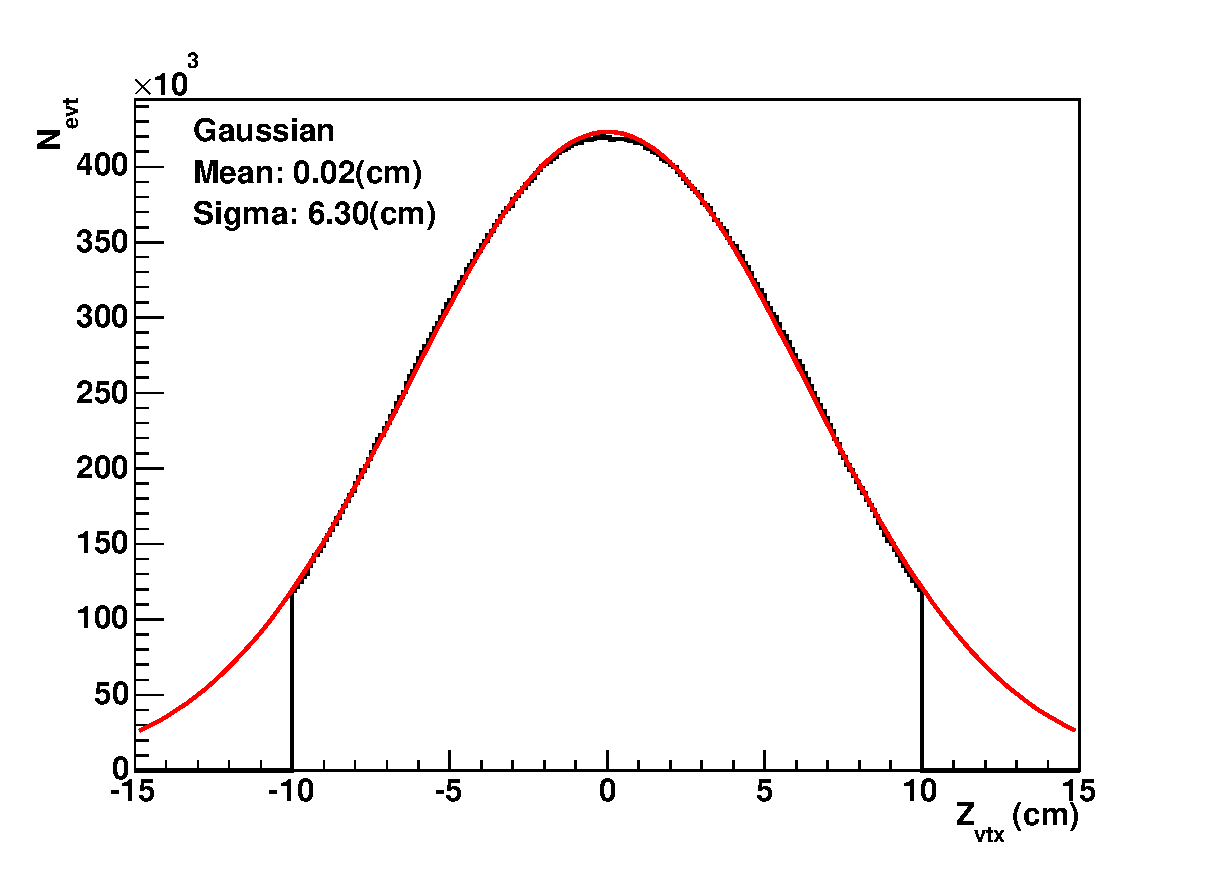
\includegraphics[width=10cm]{chap4/figure/QA/Zvtx_INT7.eps}
  \caption{$Z_{vtx}$ distribution of the accepted minimum bias events in p-Pb collisions.}
  \label{fig_4_zvtx}
\end{figure}

After the event selection, the number of selected events is 96 M events. 
The cross section of the minimum bias events triggered with V0 detector is 2.09 $\pm$ 0.06 b measured by van der Meer scan\cite{bib_v0cross}. 
Therefore the integrated luminosity is calculated as following, 
\begin{equation}
  \int{Ldt} = \cfrac{N_{MB,ana}}{\sigma_{V0}} = 96 M / 2.09 (b) = 48 \mu b^{-1}
\end{equation}

%\subsection{TRD Triggers Event Selection}
%The TRD trigger suffers from the secondary electrons from photon decays at large radii due to the straight line fit of track reconstruction as shown in Fig.~\ref{fig_4_fakeconv}. 
%\begin{figure}[!h]
%  \centering
%  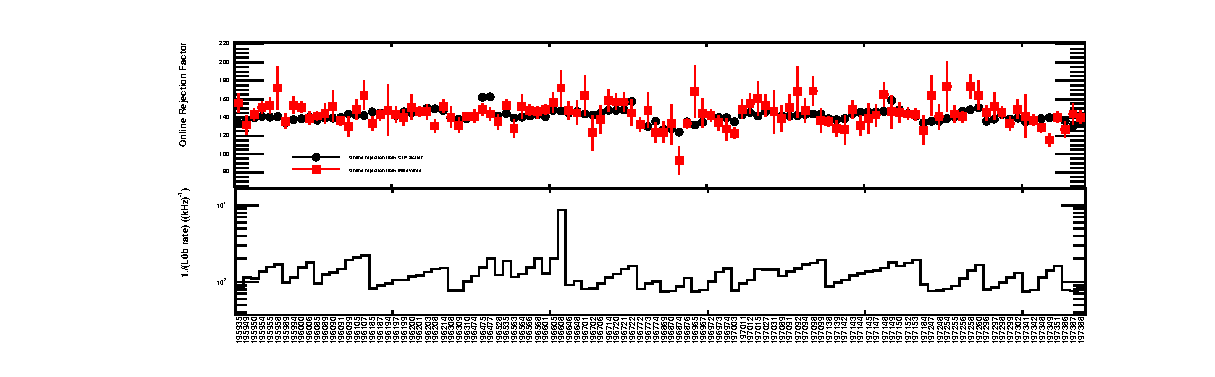
\includegraphics[width=18cm]{chap4/figure/TRDOnline/OnlineRejeandL0brate_LHC13ef.eps}
%  \caption{Run by run online event rejection factor during rare trigger runs in p-Pb collisions.}
%  \label{fig_4_}
%\end{figure}

%\begin{figure}[!h]
%  \centering
%  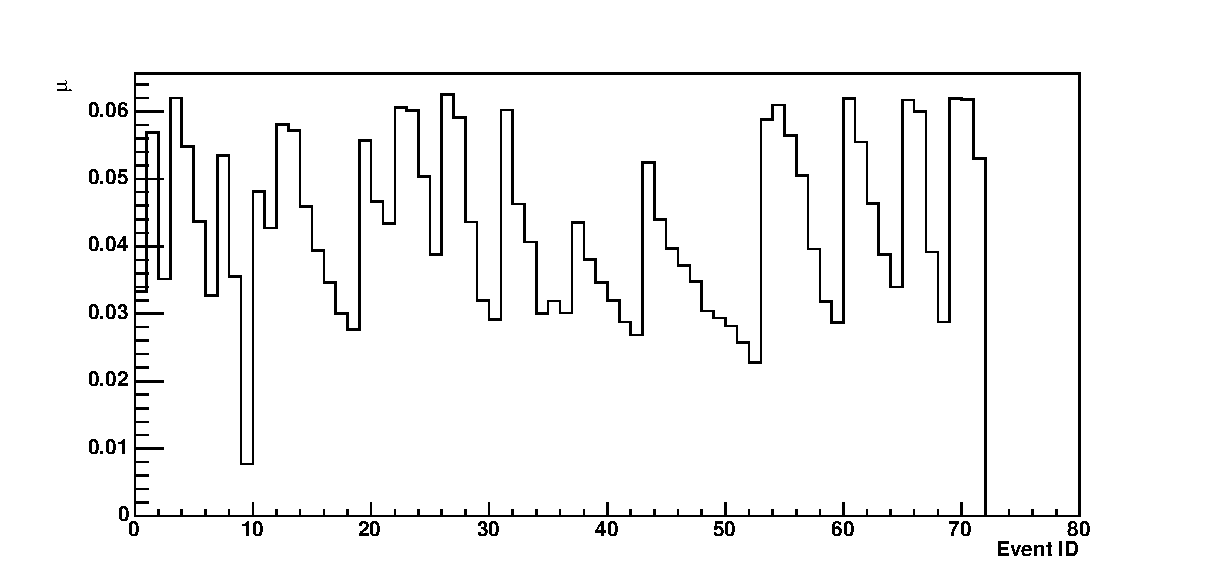
\includegraphics[width=15cm]{chap4/figure/TRDOnline/EventMu_LHC13f.eps}
%  \caption{Run by run $\mu$ of the poisson distribution.}
%  \label{fig_4_}
%\end{figure}
%\begin{figure}[!h]
%  \centering
%  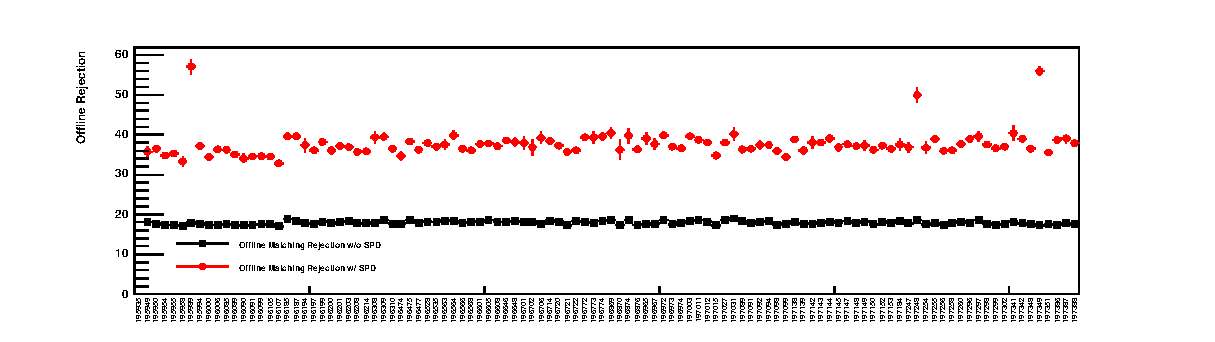
\includegraphics[width=15cm]{chap4/figure/TRDOnline/OfflineMatch_LHC13ef.eps}
%  \caption{Run by run online event rejection factor during rare trigger runs in p-Pb collisions.}
%  \label{fig_4_}
%\end{figure}
%\begin{figure}[!h]
%  \centering
%  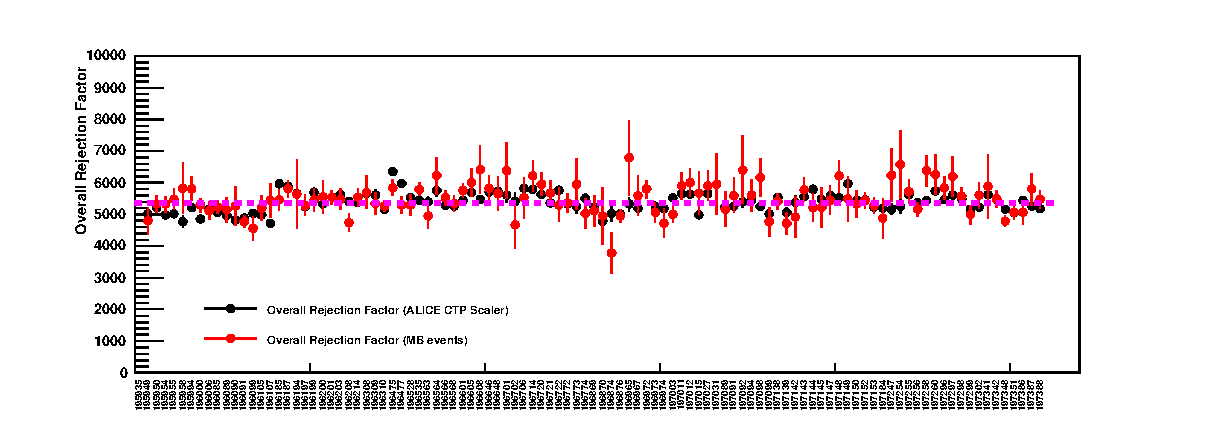
\includegraphics[width=15cm]{chap4/figure/TRDOnline/OverallRejection_LHC13ef.eps}
%  \caption{Run by run online event rejection factor during rare trigger runs in p-Pb collisions.}
%  \label{fig_4_}
%\end{figure}

%\begin{figure}[!h]
%  \centering
%  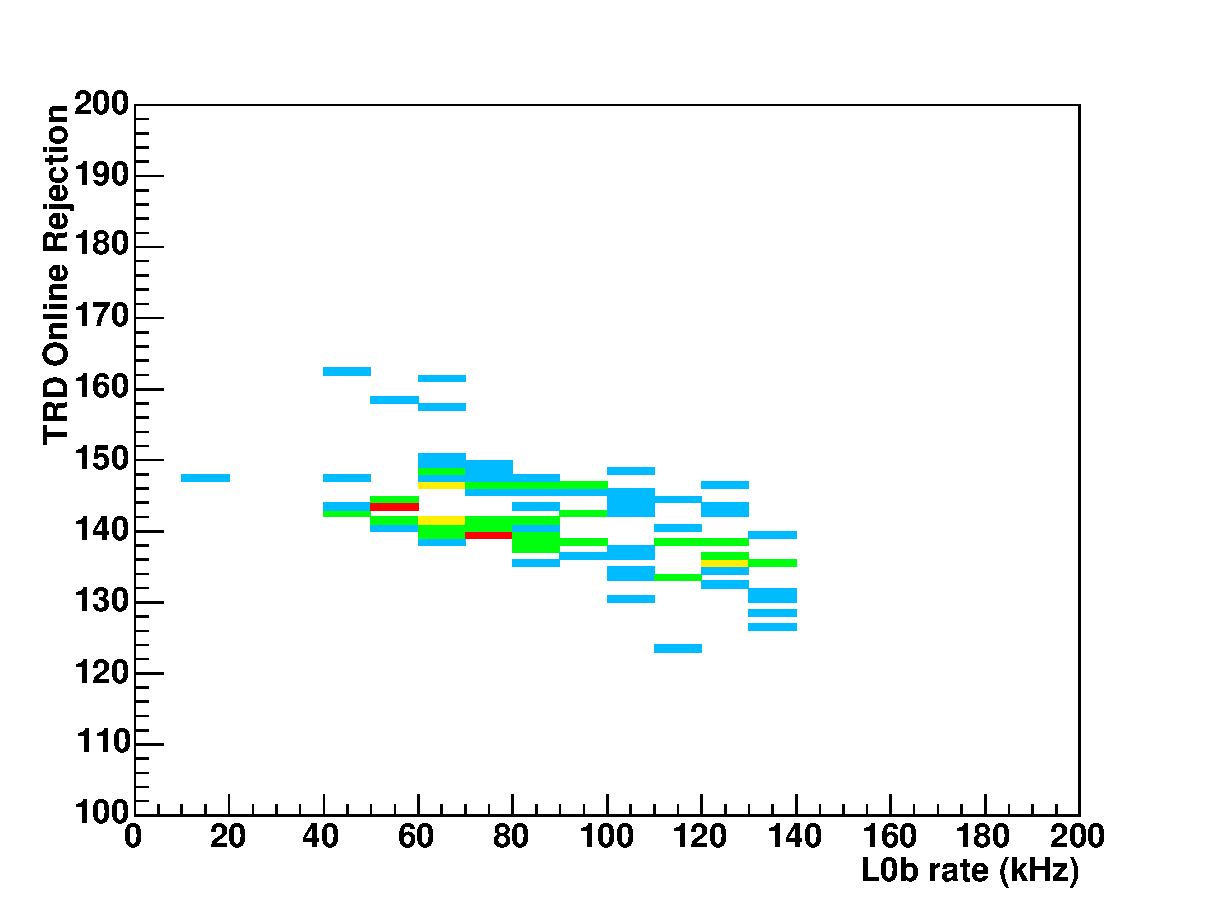
\includegraphics[width=9cm]{chap4/figure/TRDOnline/OnlineRejvsL0brate_log.eps}
%  \caption{Collision rate dependence on online rejection factor in p-Pb collisions}
%  \label{fig_4_}
%\end{figure}

%\begin{figure}[!h]
%  \centering
%  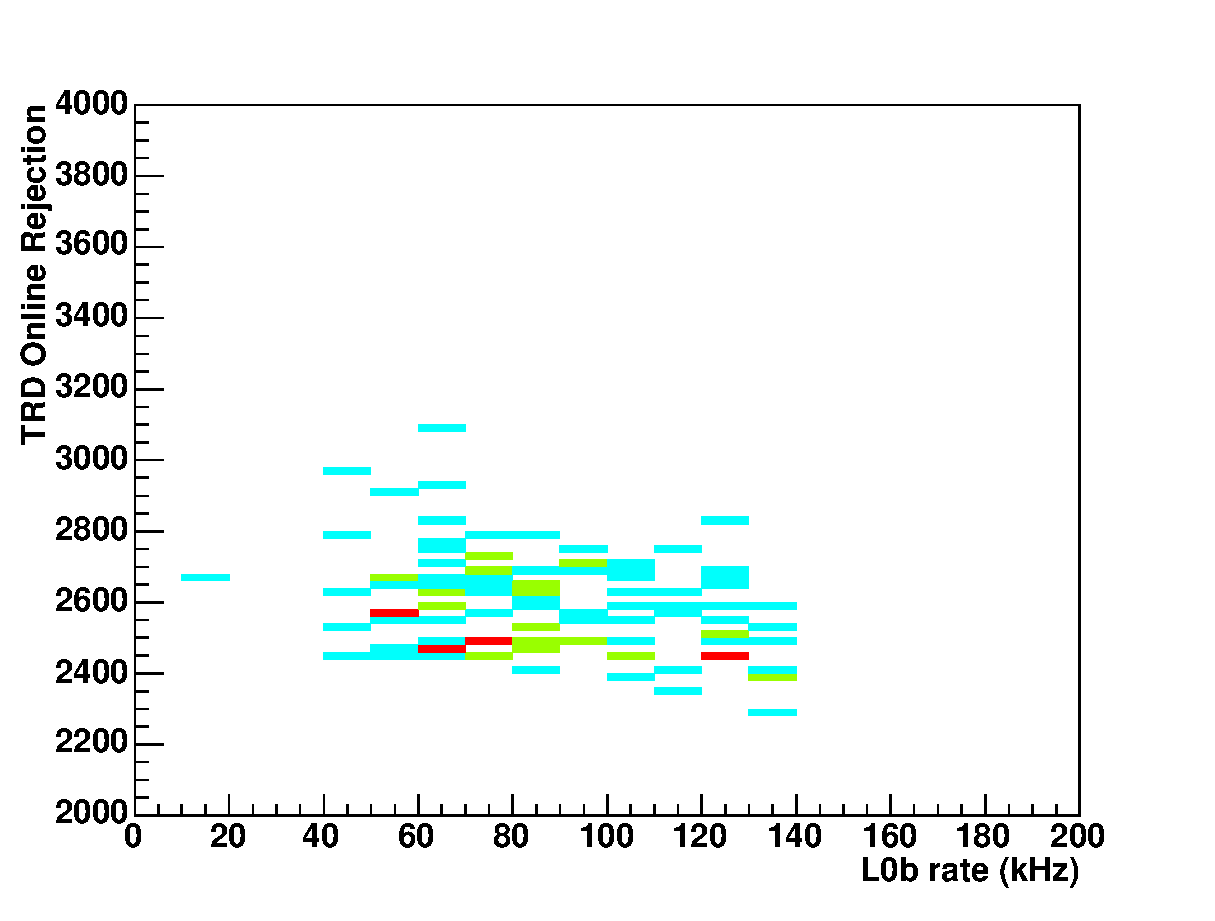
\includegraphics[width=9cm]{chap4/figure/TRDOnline/OnlineRejvsL0brateoff_log.eps}
%  \caption{Collision rate dependence on online rejection factor including offline matching in p-Pb collisions}
%  \label{fig_4_}
%\end{figure}

%\begin{figure}[!h]
%  \centering
%  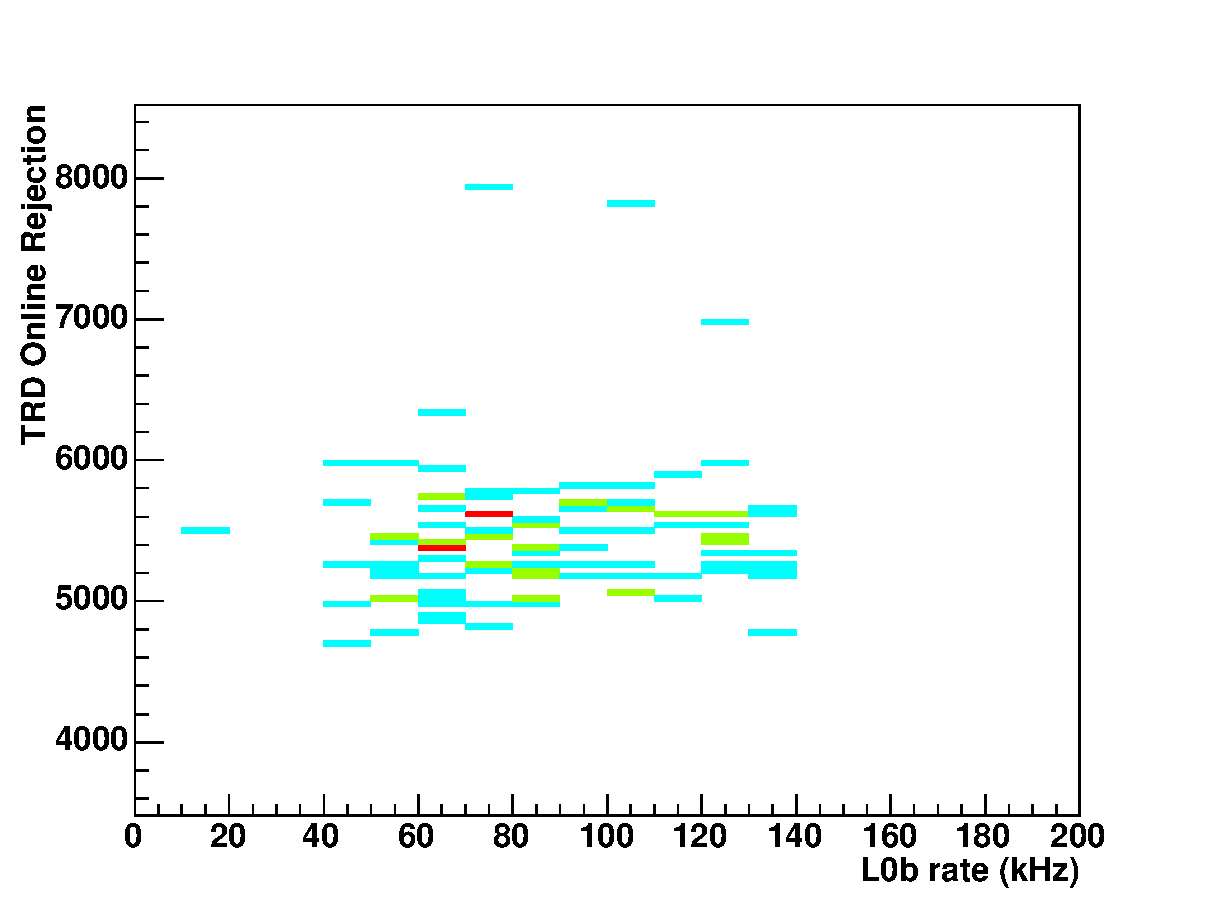
\includegraphics[width=9cm]{chap4/figure/TRDOnline/OnlineRejvsL0bratespd_log.eps}
%  \caption{Collision rate dependence on online rejection factor including SPD matching in p-Pb collisions}
%  \label{fig_4_}
%\end{figure}

%\begin{figure}[!h]
%  \centering
%  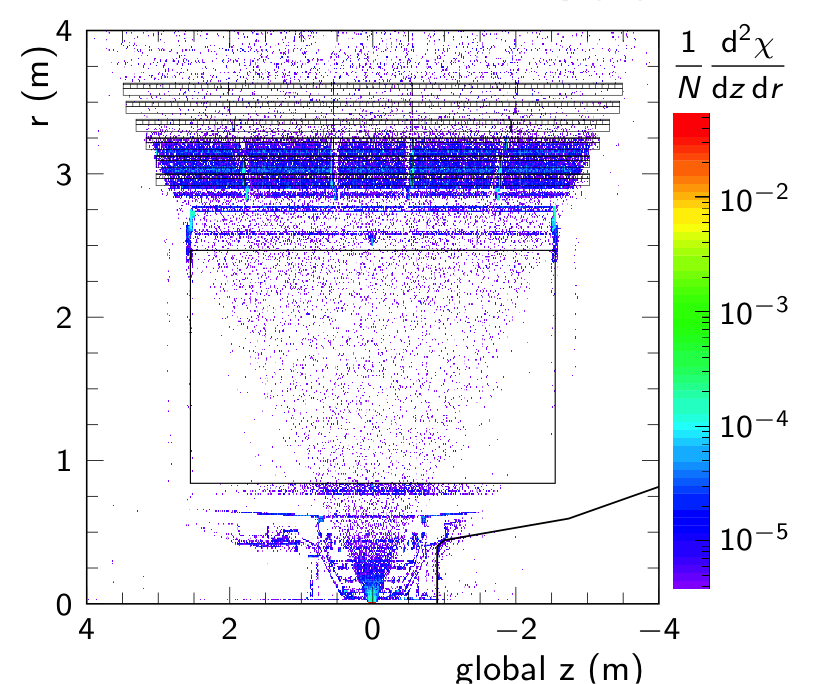
\includegraphics[width=10cm]{chap4/figure/TRDOnline/ConversionDisEta.png}
%  \caption{$\eta$ distribution of conversion electrons generated in the ALICE detectors.}
%  \label{fig_4_}
%\end{figure}

%\begin{figure}[!h]
%  \centering
%  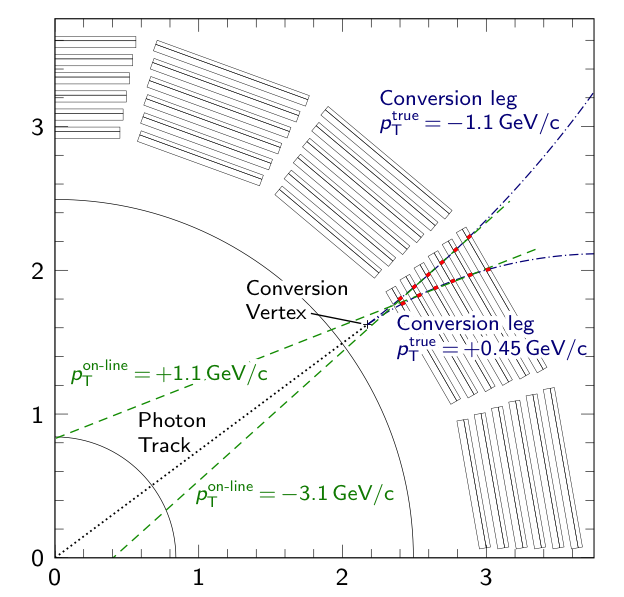
\includegraphics[width=10cm]{chap4/figure/TRDOnline/fake_conversion.png}
%  \caption{Example of fake trigger by late conversion electrons.}
%  \label{fig_4_fakeconv}
%\end{figure}
%The online rejection is determined by the pure TRD PID performance but the rate of conversion electrons. 
%In order to reduce the fake triggered events, the offline-online reconstructed track matching is required in the offline analysis. 
%Almost all fake fired electrons are produced at outer of TPC and then they are not reconstructed via ITS and TPC. 
%Figure shows the rejection of offline-online track matching ratio for each runs. 

%During TRD trigger runs, the interaction rate increased high up to 200 kHz and the out-of-bunch pileup tracks has to be taken into account because the drift time of TRD is 2 $\mu s$. 
%Figure\ref{fig_} shows the collision rate dependence of rejection factors of TRD. 
%The rejection factor become lower at high collision rate due to the out-of-bunch pileup.  
%To reduce the out-of-bunch pileup, the hit on the silicon pixel detector (SPD) is required. 
%SPD is the most inner detector of ITS. 
%The integration time of the SPD readout is 100 ns and it is enough short to reject the out-of-bunch tracks because the bunch crossing interval is 200 ns in p-Pb collisions. 

%The acceptance of TRD triggers for $J/\psi$


%\subsection{Event Characteristic Variables}
%In p-Pb collisions, it is very important to see the event activity dependence because the difference of event activity correspond to the different dynamics of collisions. 
%Multiplicity is determined in different rapidity windows. 
%At mid-rapidity ($\eta$ < 1) charge particle multiplicity is estimated using SPD tracklets defined as Section\ref{sec_3_ALICEcentral}. 
%The number of SPD tracklets is naively proportional to the charge particle multiplicity. 
%The top panels of Fig.~\ref{fig_4_spdtr_MB} show the raw SPD tracklets distribution as a function of $Z_vtx$. 
%SPD tracklets multiplicity depends on the acceptance of SPD and show the asymmetry of $Z_{vtx}$ distribution. 
%\begin{figure}[!h]
 % \centering
  %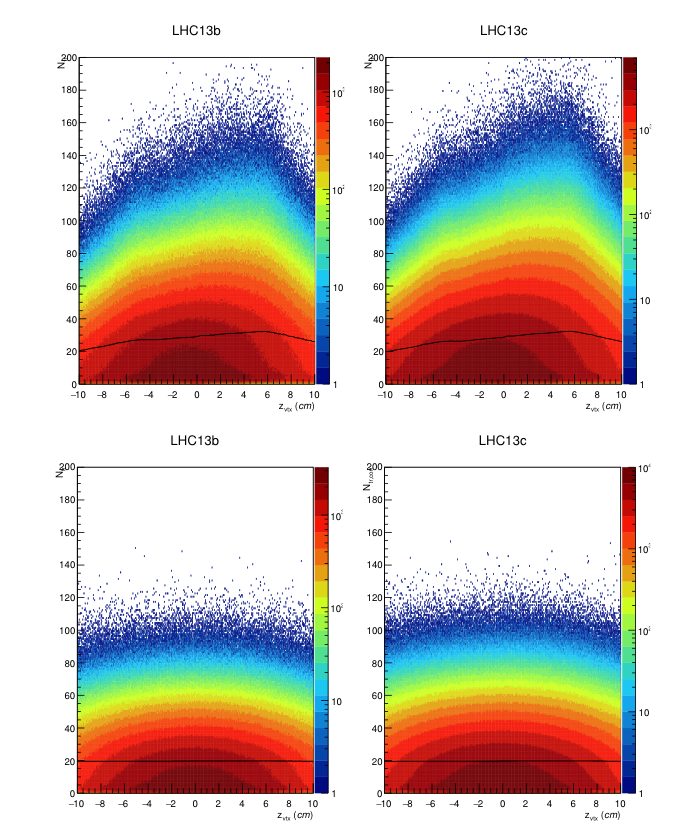
\includegraphics[width=15cm]{chap4/figure/EventActivity/SPDTracklets.png}
%  \caption{.}
%  \label{fig_4_spdtr_MB}
%\end{figure}

%In order to obtain good estimation of the charge particle multiplicity, a correction to uniform distribution for $Z_{vtx}$ is needed.
%The profile is used as an input ot renormalize $N_{tr}$ on an event-by-event-base from $<N_{tr}>$, which are 28.55 and 28.13 for LHC13b and LHC13c respectively, to the global minimum of the profile of LHC13c $<Ntr>_{glob}=$ 19.44.
%The correction factors are applied relating the global minimum to the local average $<N_{tr}>[Z_{vtx}]$ yielding from the profiles for LHC13b and LHC13c with a Poisson smearing, 
%\begin{equation}
%  \Delta_{N} = N_{tr}(\cfrac{<N_{tr}_{glob}>}{<N_{tr}>[z_{vtx}]}-1) 
%\end{equation}
%\begin{equation}
%  N^{corr}_{tr} = N_{tr} -Poisson(\Delta_{N})
%\end{equation}
%\begin{figure}[!h]
%  \centering
%  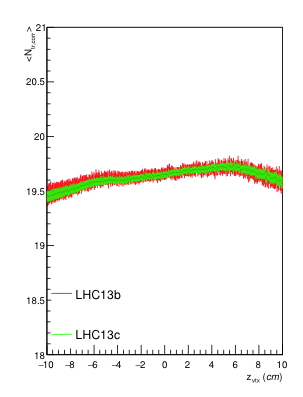
\includegraphics[width=8cm]{chap4/figure/EventActivity/MeanSPDTracklets.png}
%  \caption{.}
%  \label{fig_4_meanspdtr_MB}
%\end{figure}
%5The bottom panels of Fig.~\ref{fig_4_spdtr_MB} show the SPD tracklets multiplicity as a function of $Z_{vtx}$ after correction. 
%$<N_{tr}>$ become flat and uniform distribution is obtained in both run periods. %

%The same procedure is also done for V0A multiplicity as shown in Fig.~\ref{fig_v0atr_MB,fig_4_meanv0atr_MB}. 
%\begin{figure}[!h]
%  \centering
%  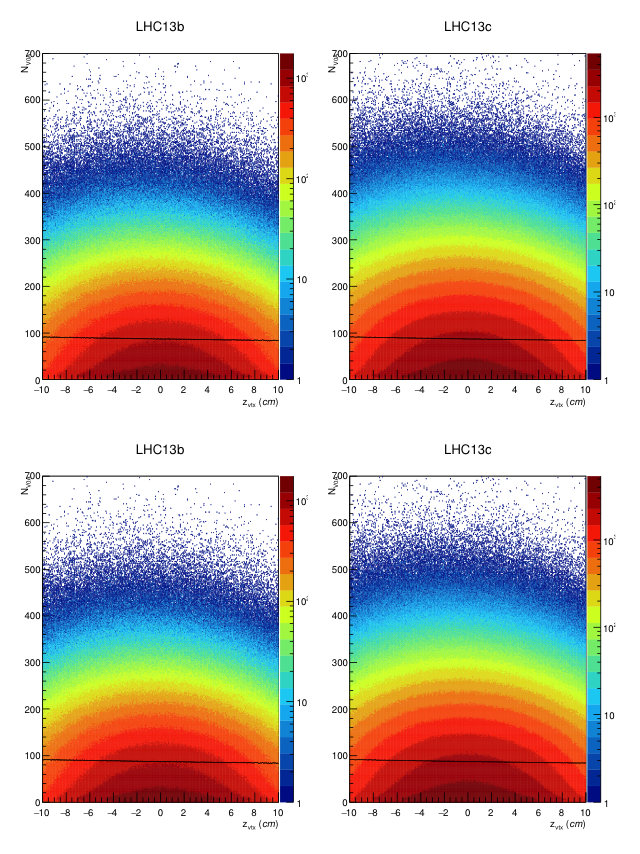
\includegraphics[width=15cm]{chap4/figure/EventActivity/V0ATracklets.png}
%  \caption{.}
%  \label{fig_4_v0atr_MB}
%\end{figure}

%\begin{figure}[!h]
%  \centering
%  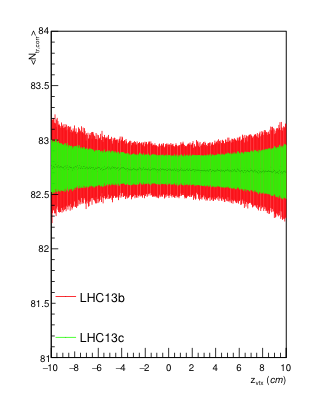
\includegraphics[width=8cm]{chap4/figure/EventActivity/MeanV0ATracklets.png}
%  \caption{.}
%  \label{fig_4_meanv0atr_MB}
%\end{figure}

%For the conversion of the corrected $N^{corr}_tr$ to $dN_{ch}/d\eta$ Monte-Carlo information is needed. 
%%In the dedicated MC samples we can count the number of charged particle tracks in .
%The $dN_{ch}/d\eta$ vs $N^{corr}_{tr}$ is plotted in Fig.\ref{fig_4_nchvsntr_MB}. 
%To obtain the linear dependence, a linear fit is done on the 2D distribution and each multiplicity intervals as shown in Fig.~\ref{fig_4_nchvsntr_MB} and $dN_{ch}/d\eta$ is calculated in each interval. 
%The relative deviation du to the perfect correction of $N^{corr}_{tr}$ is treated as a systematic uncertainty on the multiplicity variable.

%\begin{figure}[!h]
%  \centering
%  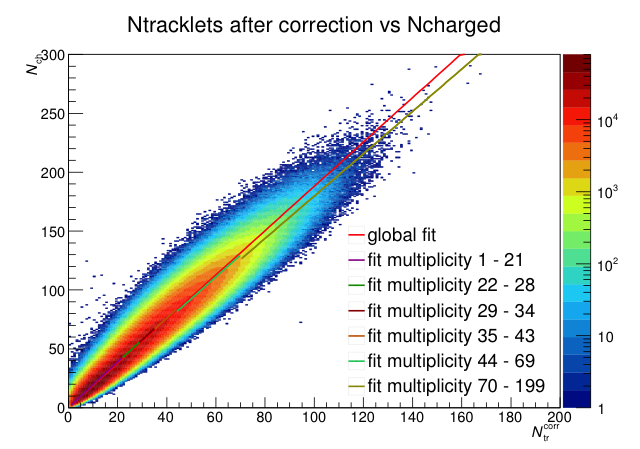
\includegraphics[width=10cm]{chap4/figure/EventActivity/NchvsNtr.png}
%  \caption{.}
%  \label{fig_4_nchvsntr_MB}
%\end{figure}


\section{Run Quality Check}
\label{sec_4_runselection}
Run quality check based on the number of electron candidates per event is performed. 
Figure~\ref{fig_4_runqa_MB} shows the number of electron candidates after the electron identification divided by the number of analyzed events for each event in minimum bias run periods in $p_{\rm{T}}=$ 1-2  GeV/$c$, $p_{\rm{T}}=$ 2-4 GeV/$c$, and $p_{\rm{T}}>4$ GeV/$c$ bins, respectively. 
The electron candidates are selected with the track quality cut summarized in Table.~\ref{table_4_trackquality} and TPC inclusion cut $|\rm{n}\sigma_{ele}| < $ 3 and TPC exclusion cuts $|\rm{n}\sigma_{pi}| < $ 3.5, $|\rm{n}\sigma_{pro}| < $ 3.5 described in Section~\ref{sec_4_eid}.
Figure~\ref{fig_4_runqapro_MB} also shows the projection of the number of electron and positron sum per event for each run. 
These distributions are well described by Gaussian.
All runs are within 5 $\sigma$ from the mean points in all categories and then all runs are accepted.  

\begin{figure}[!h]
  \centering
  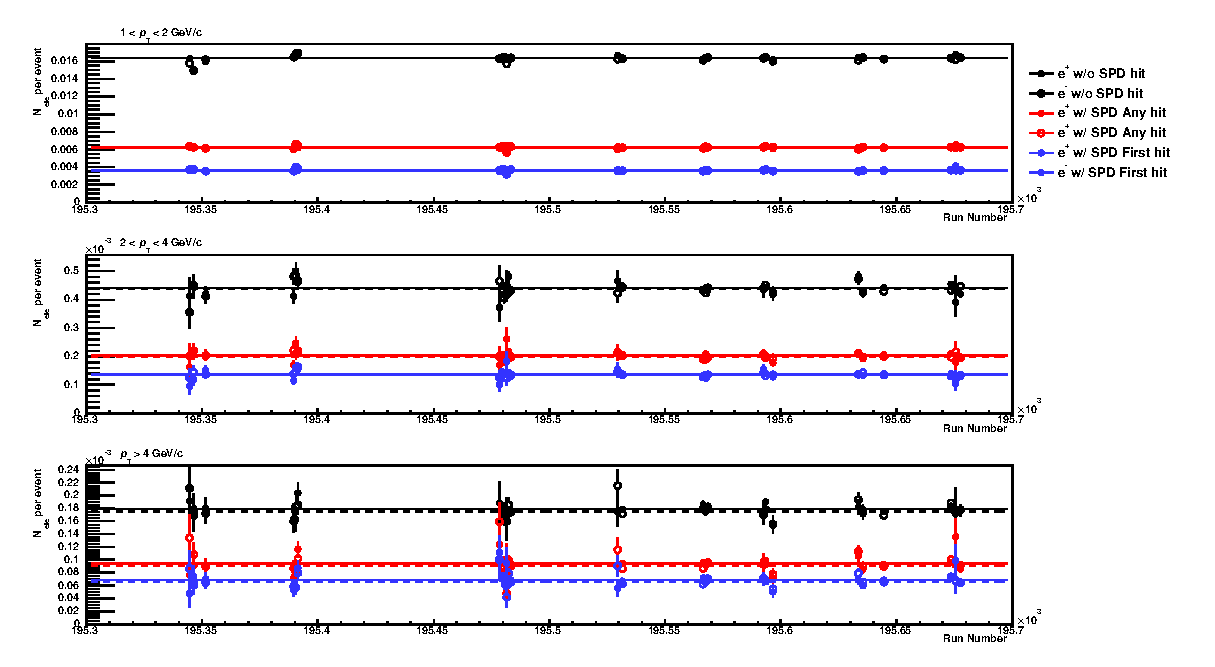
\includegraphics[width=16cm]{chap4/figure/QA/RunbyRunQA_MB.eps}
  \caption{The number of accepted tracks per event after the typical track quality and electron identification cuts for each run. From left to right, the $p_{\rm{T}}$ bins are $p_{\rm{T}}=$ 1-2 GeV/$c$, $p_{\rm{T}}=$ 2-4 GeV/$c$, and $p_{\rm{T}}>4$ GeV/$c$, respectively. The black line show the result without SPD hit requirement. The red and blue marker show results with SPD Any and SPD First requirement described in Section~\ref{sec_4_trackrec}. }
  \label{fig_4_runqa_MB}
\end{figure}
\begin{figure}[!h]
  \centering
  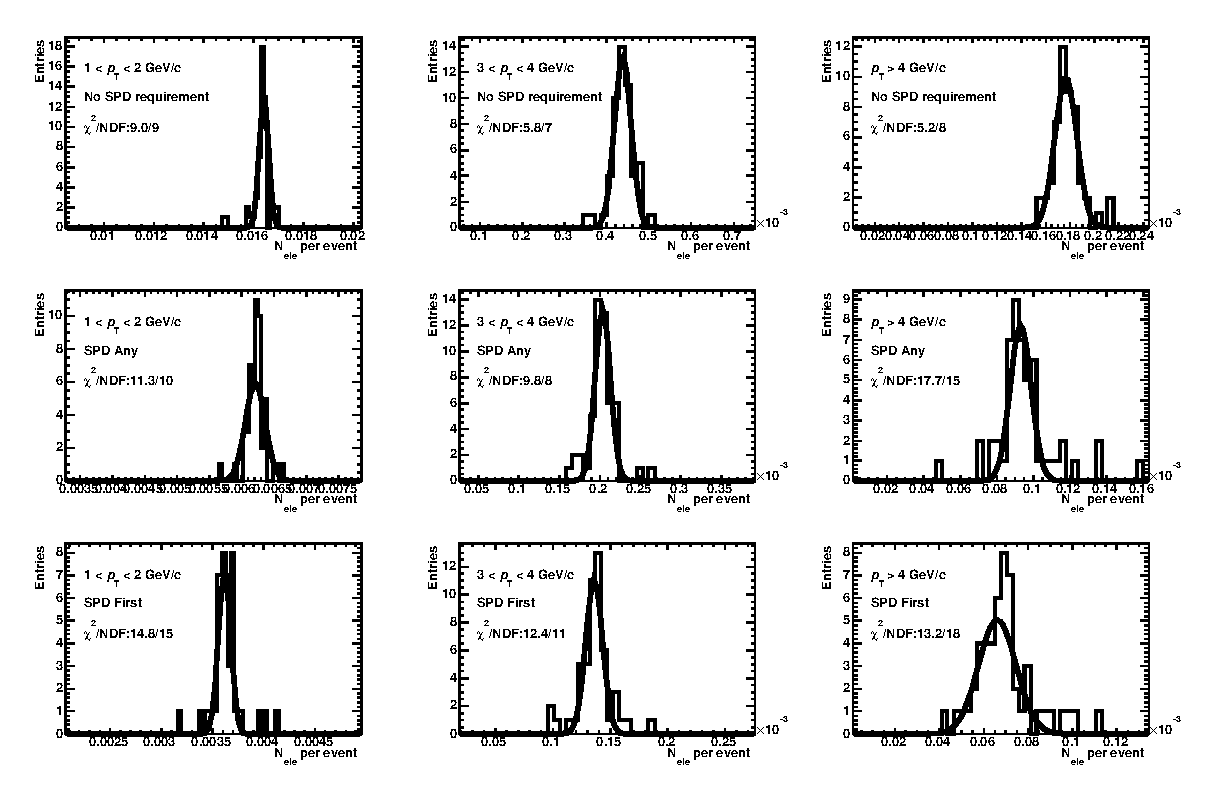
\includegraphics[width=16cm]{chap4/figure/QA/RunbyRunQAPro_MB.eps}
  \caption{The Projection of the number of accepted tracks after the typical track quality and electron identification cuts for each run and the fitting results. The results contain both electron and positron candidates. }
  \label{fig_4_runqapro_MB}
\end{figure}
%The similar check is also done for the TRD triggered data samples. 
%The typical $p_{T}$ range is different from minimum bias samples because the different kinematic ranges are aimed. 
%Some runs show discrepancy in both lower and higher samples. 
%The runs which are out of 3 $\sigmas$ from mean in both $p_{T}$ range are rejected.

%\begin{figure}[!h]
 % \centering
 % 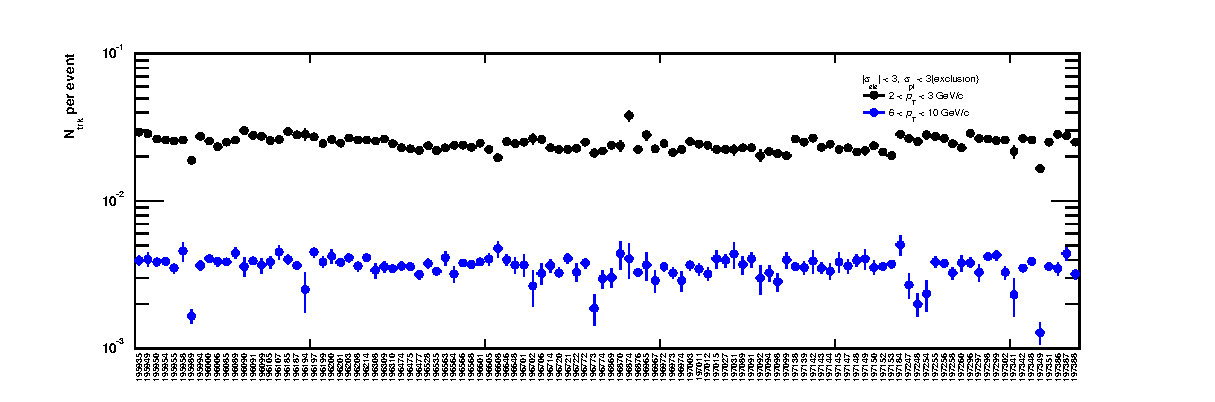
\includegraphics[width=15cm]{chap4/figure/QA/RunByRunPIDQA_TRDTrigger.eps}
 % \caption{The number of accepted track after typical track quality and electron identification cuts for each TRD trigger runs.}
 % \label{fig_4_runqa_Trigger}
%\end{figure}

\section{Track Selection}
\label{sec_4_trackrec}
\subsection{Kinematic Selection}
Kinematical selection of such as $p_{\rm{T}}$ and $\eta$ is investigated using single $J/\psi$ simulation. 
The left panel of Fig.~\ref{fig_4_legptkin} shows $p_{\rm{T}}$ distribution of leg electrons which have higher $p_{\rm{T}}$ than the other one. 
The right panel of Fig.~\ref{fig_4_legptkin} shows $p_{\rm{T}}$ distribution of leg electrons with lower $p_{\rm{T}}$. 
Since $J/\psi$ has the invariant mass of 3.096 GeV/$c^{2}$, both electrons have relatively high $p_{T}$ ($\sim$ 1.5 GeV/$c$) with large opening angle at low mother $p_{T}$.  
At intermediate mother $p_{T}$, one leg electron carries a large part of mother's momentum compared to the other one. 
\begin{figure}[!h]
  \centering
  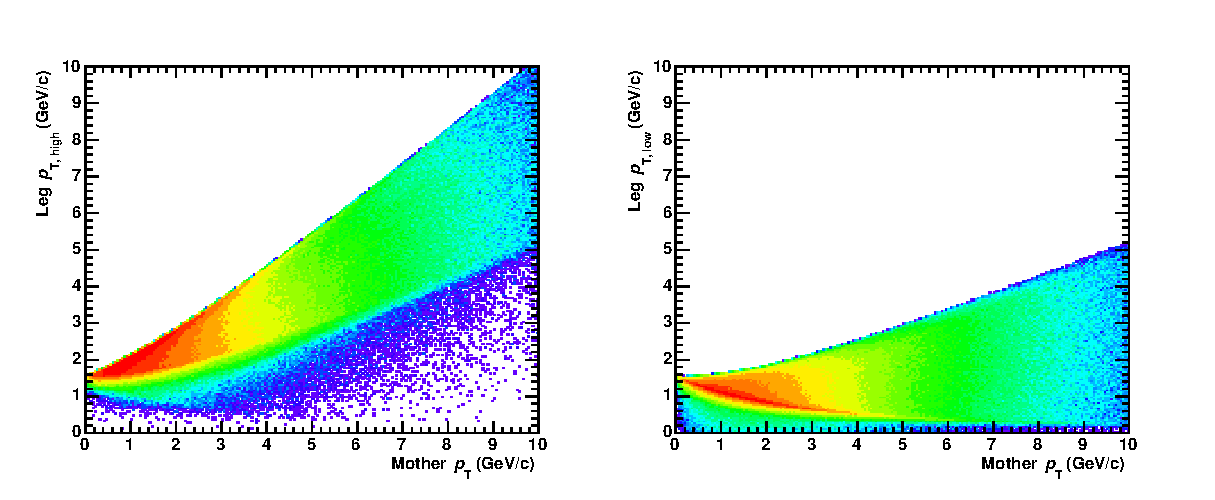
\includegraphics[width=16cm]{chap4/figure/Kinematics/Jpsi_mompt_legpt.eps}
  \caption{ $p_{T}$ distribution of leg electrons with higher $p_{T}$ (Left) and lower $p_{T}$ (Right) from $J/\psi$ decays as a function of mother $p_{T}$ in Monte-Carlo simulation. }
  \label{fig_4_legptkin}
\end{figure}

Figure~\ref{fig_4_single} shows the inclusive electron spectrum and the expected population of each source. 
At lower $p_{\rm{T}}$ below 1 GeV/c, light hadron decay and conversion electrons which are generated in the material of the detectors from real photons are dominant. 
\begin{figure}[!h]
  \centering
  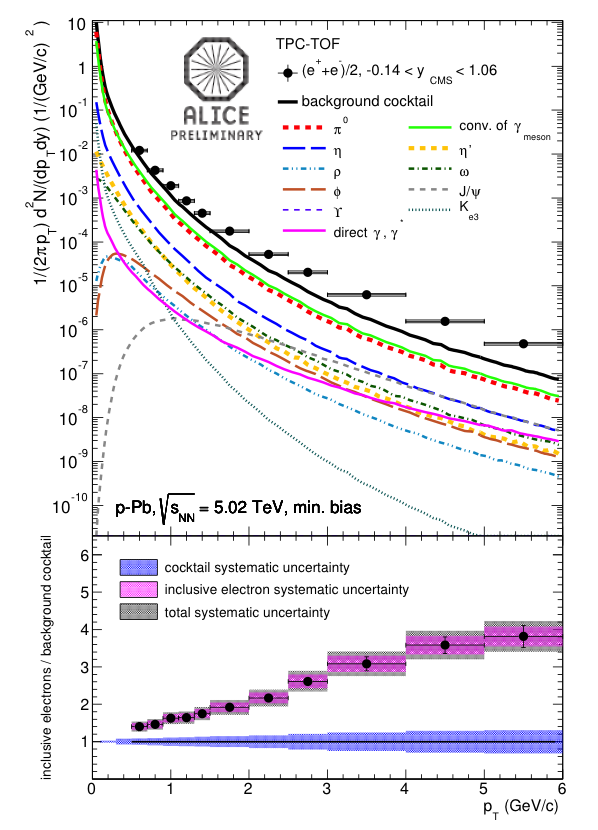
\includegraphics[width=8cm]{chap4/figure/Kinematics/single.png}
  \caption{Inclusive single electron spectrum and the population of each source in p-Pb collisions. }
  \label{fig_4_single}
\end{figure}
In order to keep good signal to background ratio for $J/\psi$, the combinatorial background generated by electrons from light hadron decays and material conversion is needed to be suppressed. 
In this analysis, the following kinematic selection is applied, 
\begin{itemize}
  \item $p^{e}_{T}>1~GeV/c$ 
  \item $|\eta^{e}|<0.9$
\end{itemize}
In case $p_{T}$ differential analysis, leg $p_{T}$ cut is also optimized to increase the significance ans cut parameters are summarized in Table~\ref{table_4_cutset}. 
Figure~\ref{fig_4_jpsiacce} shows the kinematic acceptance of $J/\psi$ in Monte-Carlo simulation. 

The kinematic acceptance is defined as following, 
\begin{equation}
  \epsilon_{kin} = \cfrac{ \rm{The~number~of~}  J/\psi \rm{~after ~leg }~\it{p}_{\rm{T}} \rm{~and }~\eta\rm{ ~cuts~ in} ~|\it{y}|~ <~\rm{0.9}}
          {\rm{The~ number~ of~ generated~} J/\psi \rm{~in~} |\it{y}| ~<~ \rm{0.9}}
\end{equation}
Above kinematical selection still keeps the acceptance for $J/\psi$ from low $p_{\rm{T}$ to high $p_\rm{T}$.
\begin{figure}[!h]
  \begin{minipage}{0.5\hsize}
    \begin{center}
      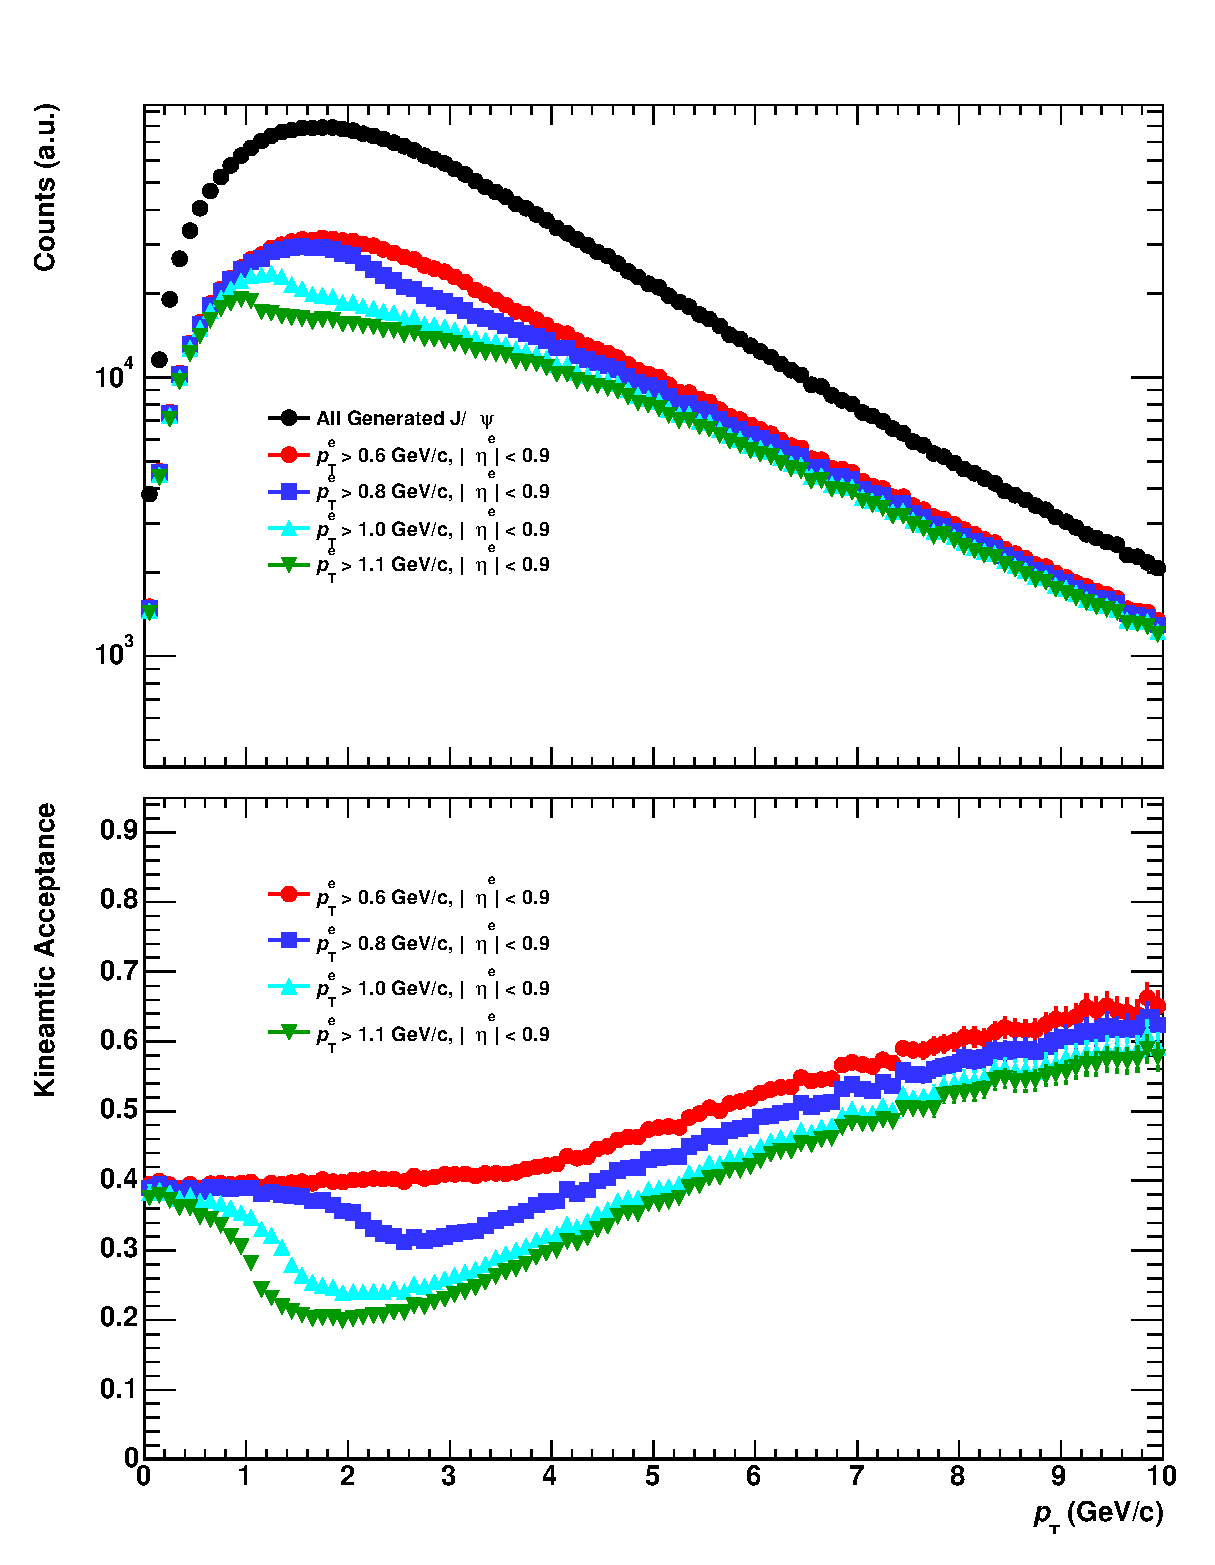
\includegraphics[width=8cm]{chap4/figure//Kinematics/MCJpsi_ptacce.eps}
    \end{center}
  \end{minipage}
  \begin{minipage}{0.5\hsize}
    \begin{center}
      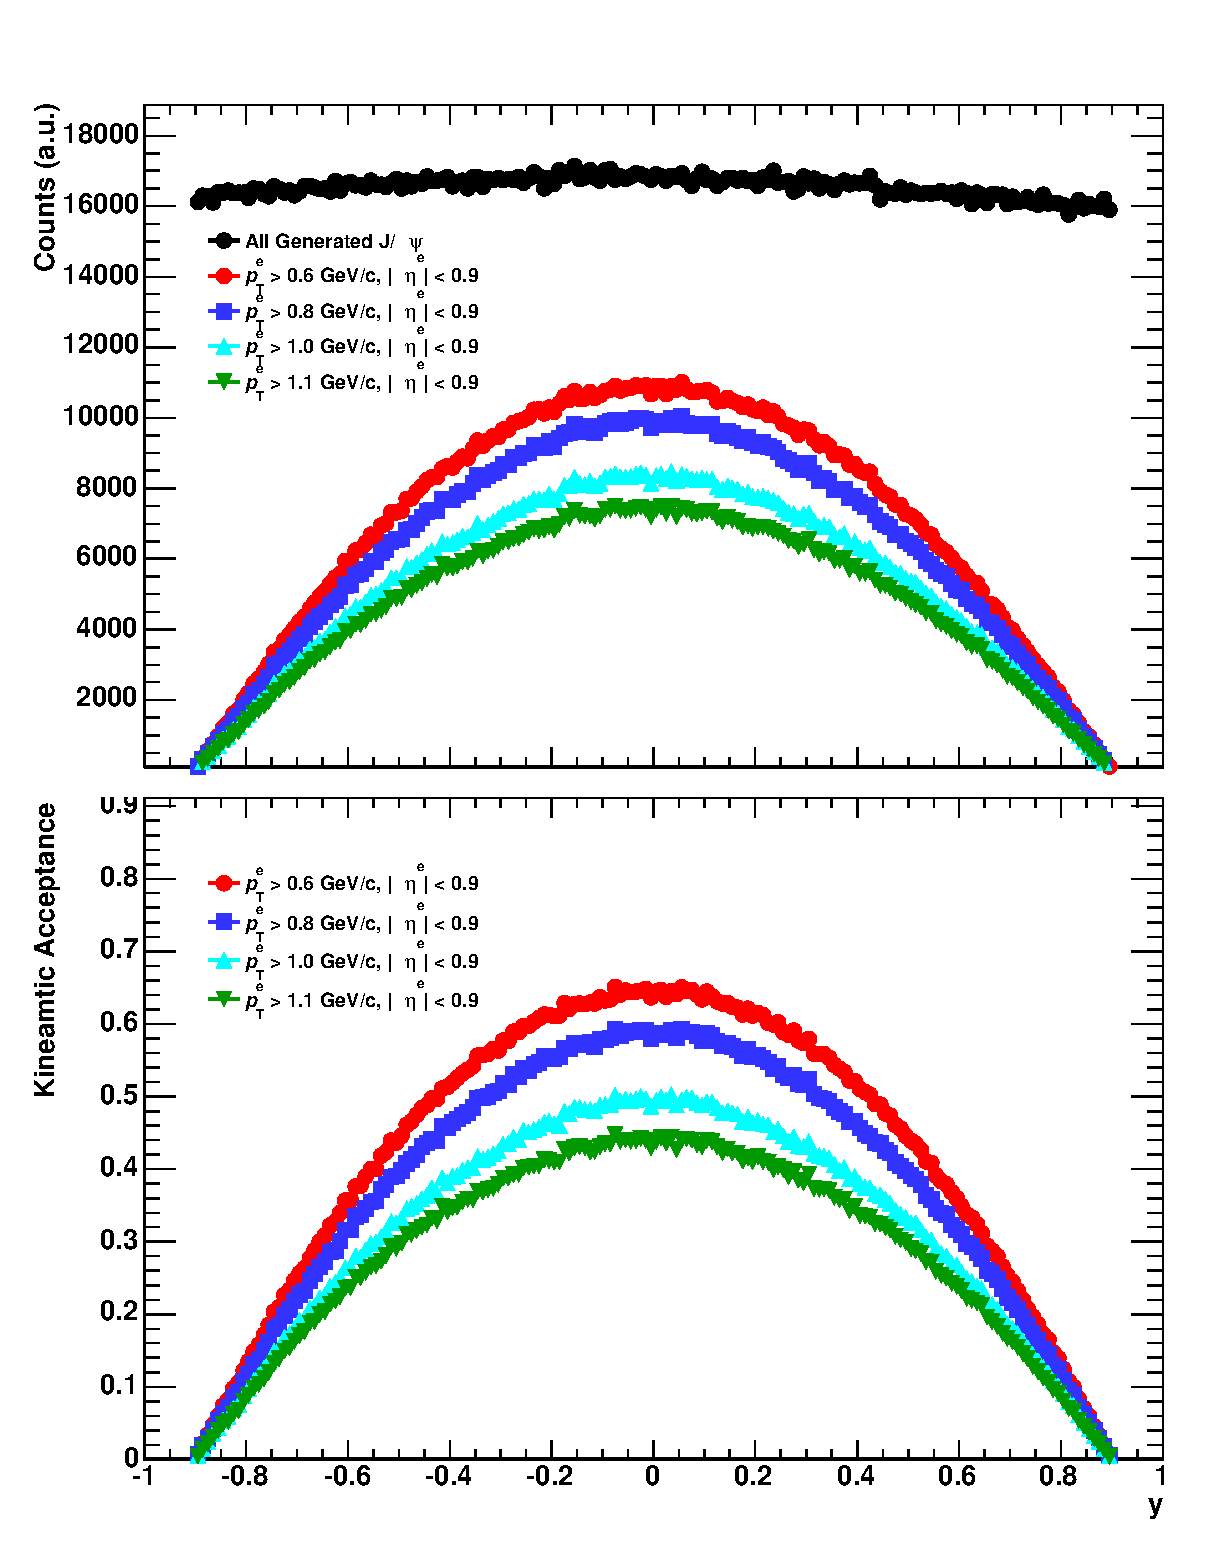
\includegraphics[width=8cm]{chap4/figure//Kinematics/MCJpsi_yacce.eps}
    \end{center}
  \end{minipage}
  \caption{
    Kinematic acceptance for J/$\psi$ as a function of $p_{T}$ (Left) and y (Right) in Monte-Carlo simulation.
  }
  \label{fig_4_jpsiacce}
\end{figure}


\subsection{Track Quality Cuts}
\begin{table}[!h]
  \centering
  \begin{tabular}{lc} \hline
    Cut   & Value \\ \hline
    Minimum leg $p_{T}$  & $>$ 1 GeV/c \\ \hline
    $|\eta^{e}_{lab}|$  & $<$ 0.9 \\ \hline
    refit  &  ITS and TPC\\ \hline
    The number of TPC clusters (TPC $N_{cls}$) & $>$ 70 \\ \hline
    TPC $\chi^{2}/N_{cls}$ & $<$ 4 \\ \hline
    $|DCA_{XY}|$ & $<$ 1 cm \\ \hline
    $|DCA_{Z}|$ & $<$ 3 cm \\ \hline
  \end{tabular}  
  \caption{Summary of cut setting for track reconstruction. }
\label{table_4_trackquality}
\end{table}
Charged tracks are reconstructed using hits on ITS and TPC as described in Section~\ref{sec_3_trackrec}.
In order to select good track samples, ITS and TPC quality cuts are applied. 
All tracks are required to be re-fitted as described in Section~\ref{sec_3_trackrec}
The loose impact parameter cuts for XY plane and Z axis are also applied ($DCA_{XY} <$ 1 cm, $DCA_{Z} < $ 3 cm).  
The impact parameter is defined as the distance between tracks and the primary vertex when tracks propagate to the primary vertex.  
Figure~\ref{fig_4_qa_tpc} show the distribution of the number of TPC clusters and $\chi^{2}$ between reconstructed tracks and the associated TPC clusters divided by the number of TPC clusters of electron candidates. 
They are selected by electron inclusion and pion exclusion cuts of TPC $dE/dx$ described in Section.~\ref{sec_4_eid}. 
\begin{figure}[!h]
  \centering
  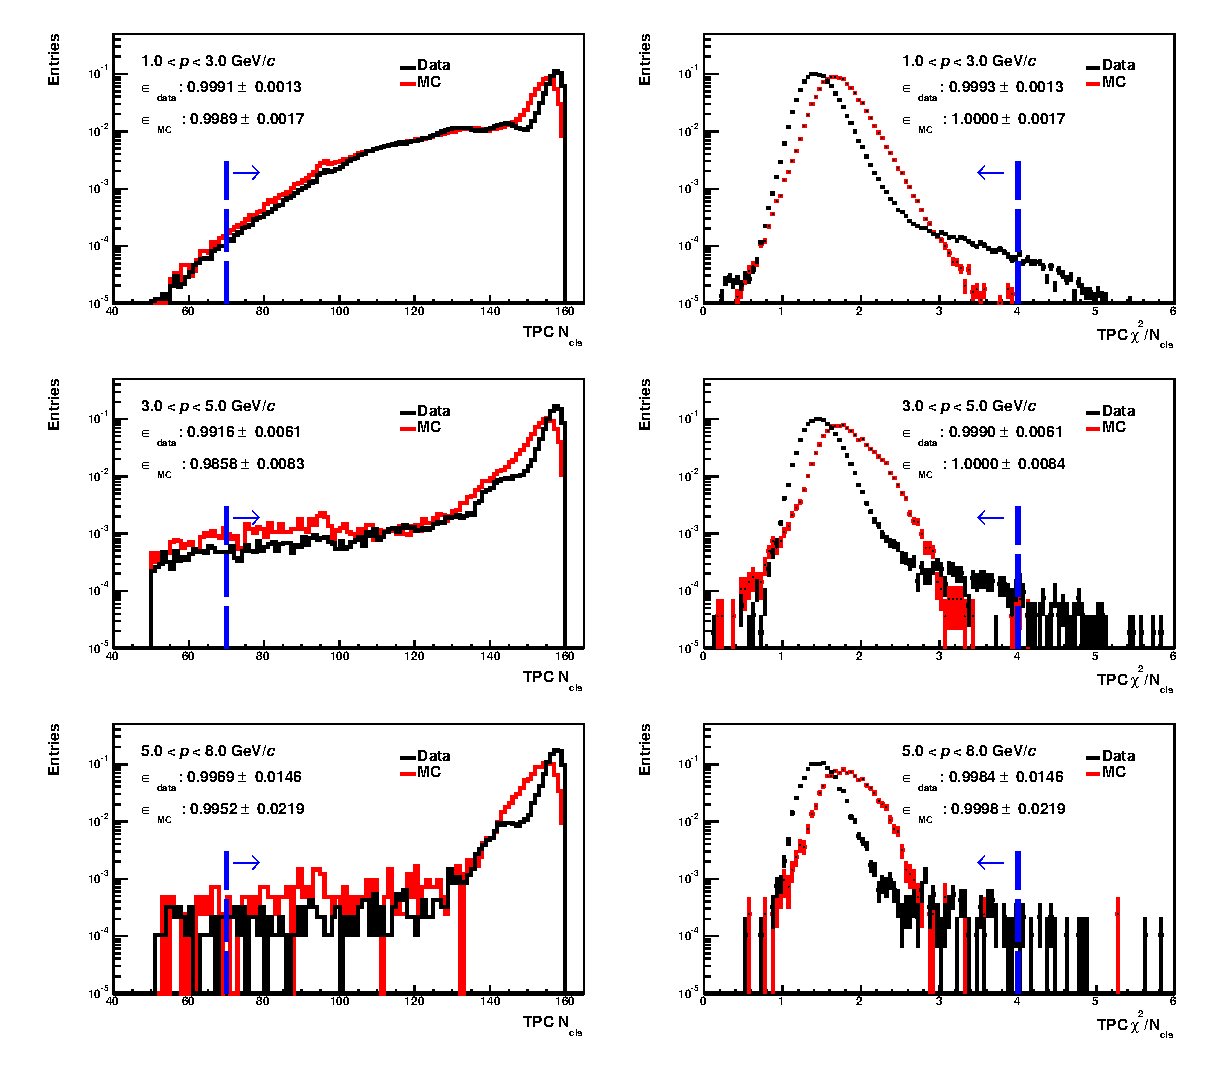
\includegraphics[width=15cm]{chap4/figure/TrackQA/TPCNclsandChi2_LHC13befix2.eps}
  \caption{Distribution of the number of TPC clusters (Left) and TPC $\chi^{2}$ divided by the number of TPC clusters (Right) for electron samples in 3 momentum ranges. The black lines show the result of the real data and the red lines show the result of Monte-Carlo simulation. The dashed lines show the thresholds of the track selection cuts.}
  \label{fig_4_qa_tpc}
\end{figure}
There are clear discrepancies between the experimental data and Monte-Carlo simulation. 
However tracks are required at least 70 clusters out of maximum 159 hits and $\chi^{2}$ per TPC clusters below 4. 
Therefore integrated efficiency calculated by the Monte-Carlo simulation is identical with the analyzed data.
\begin{figure}[!h]
  \centering
  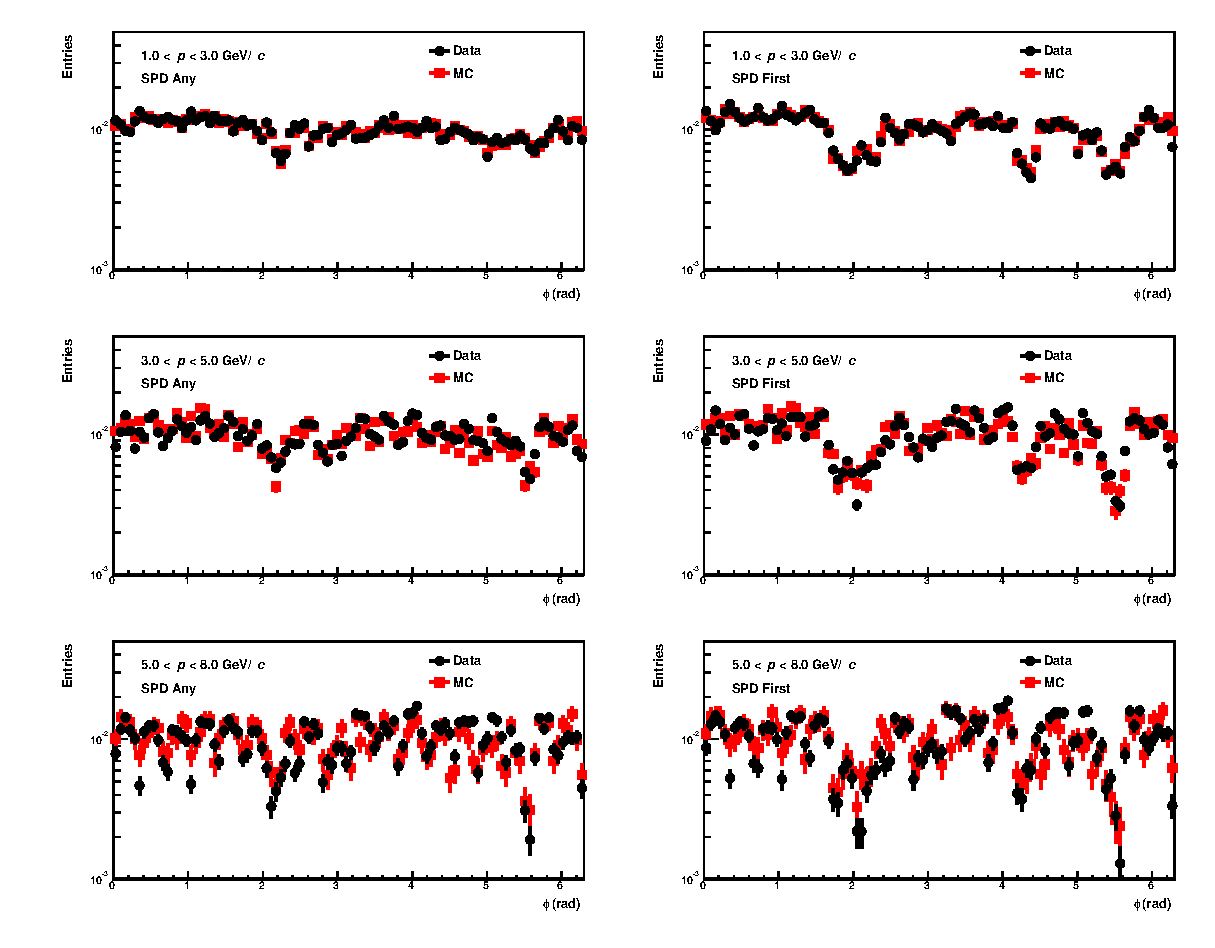
\includegraphics[width=15cm]{chap4/figure/TrackQA/Phi_tof3_tpc2_tpcpi3_MB.eps}
  \caption{$\phi$ distribution of electron samples after SPD Any (Left) and First (Right) requirements. The black markers show the result of the real data and the red markers show the result of Monte-Carlo simulation.}
  \label{fig_4_qa_phi}
\end{figure}

\begin{figure}[!h]
  \centering
  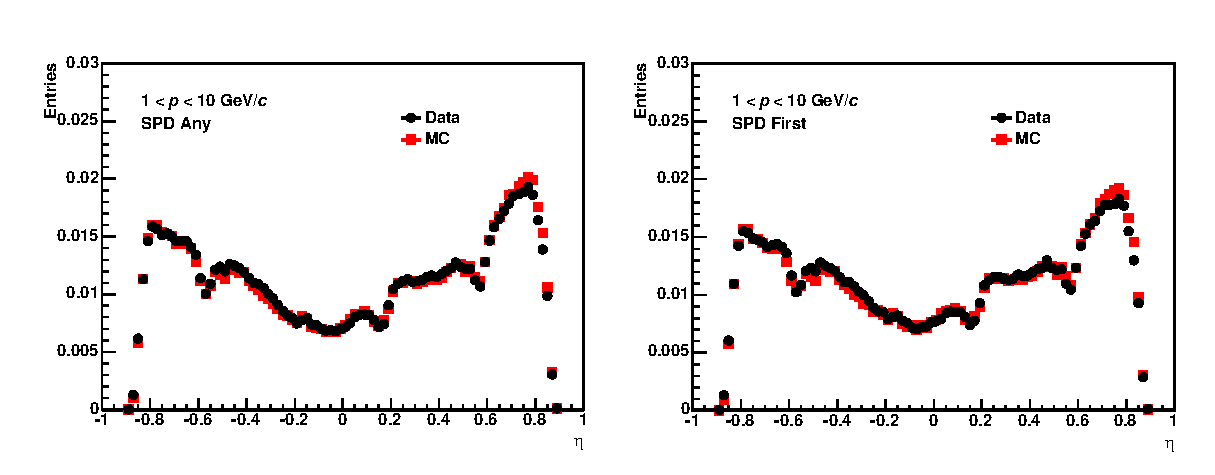
\includegraphics[width=15cm]{chap4/figure/TrackQA/Eta_tof3_tpc2_tpcpi3_MB.eps}
  \caption{$\eta$ distribution of electron samples after SPD Any (Left) and First (Right) requirements. The black markers show the result of the real data and the red markers show the result of Monte-Carlo simulation.}
  \label{fig_4_qa_eta}
\end{figure}

For the rejection of conversion electrons, hits on the SPD layers are required since the conversion electrons generated at large radii such as SSD, SDD, and TPC are suppressed by this requirement. 
SPD also has a fast integration time ($\sim$100 ns) compared to the bunch spacing (200 ns in p-Pb case) and then the contribution from out-of-bunch is negligible by the SPD hit requirement. 
Figures~\ref{fig_4_qa_phi} and ~\ref{fig_4_qa_eta} show the $\phi$ and $\eta$ distributions of reconstructed tracks after the SPD Any and First requirements. 
SPD Any means at least one hit on SPD layers is required while SPD First means a hit on the first layer of SPD is required. 
There is a good agreement between the analyzed data and Monte-Carlo simulations. 

\begin{figure}[h]
 \begin{minipage}{0.5\hsize}
  \begin{center}
  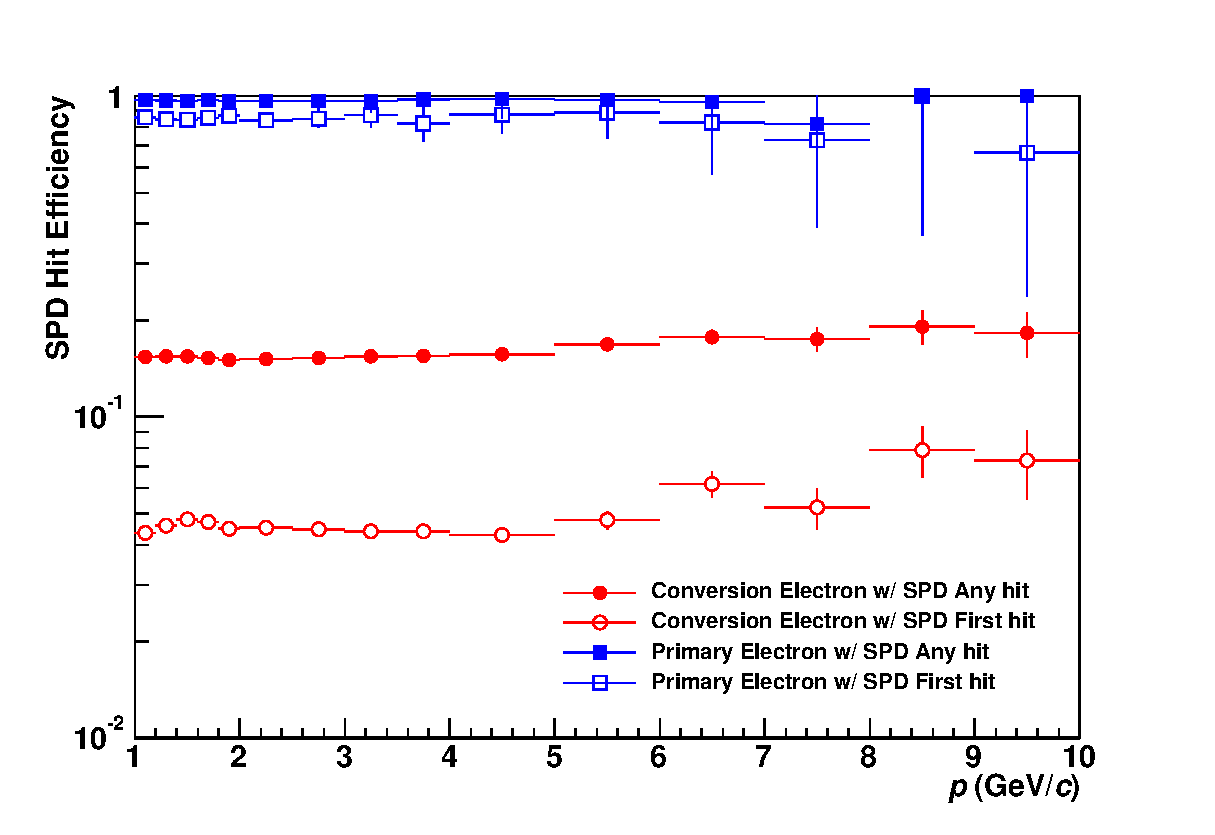
\includegraphics[width=8cm]{chap4/figure/TrackQA/SPDHit/SPDHitEff_PrimeConv_MB.eps}
  \end{center}
 \end{minipage}
 \begin{minipage}{0.5\hsize}
  \begin{center}
    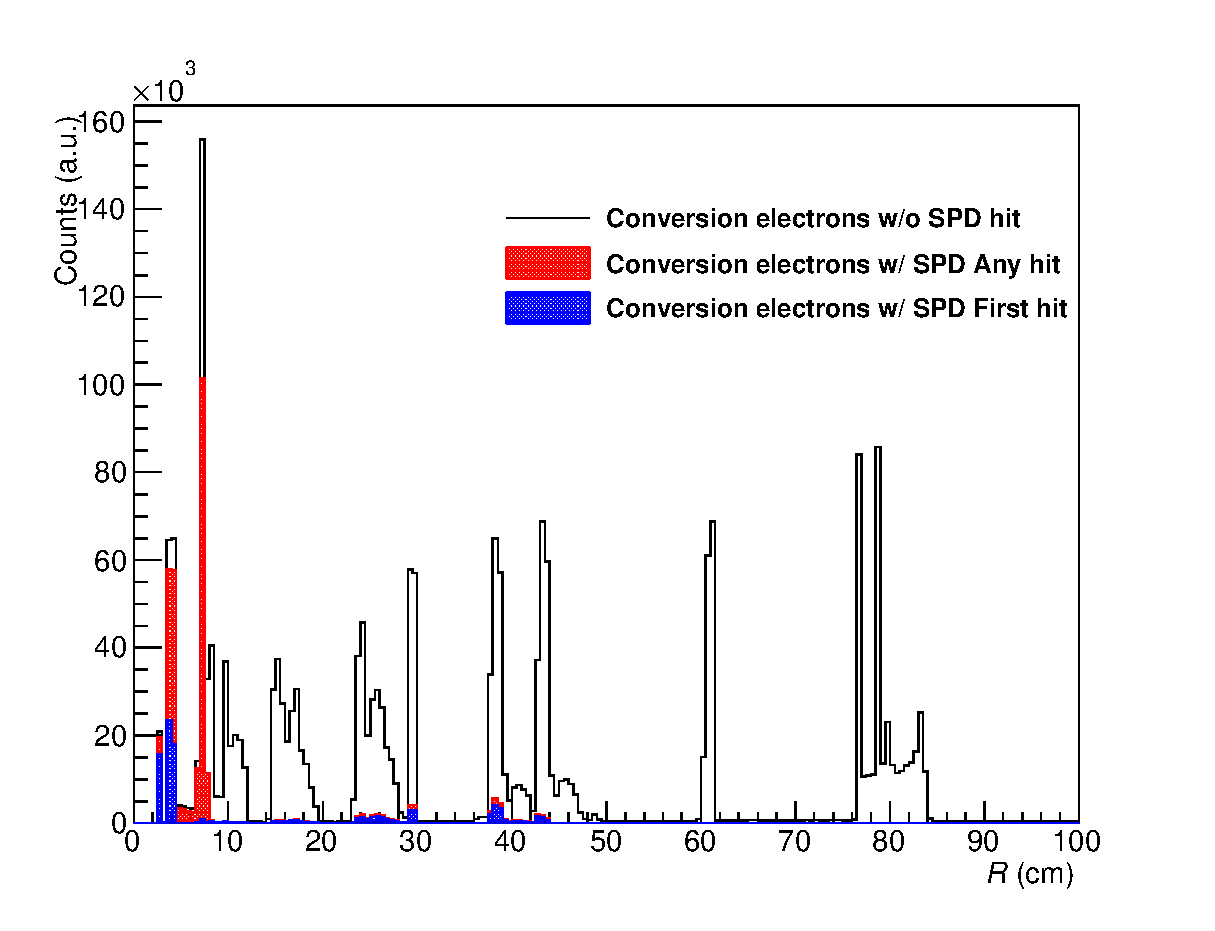
\includegraphics[width=8cm]{chap4/figure/TrackQA/SPDHit/ConvRDistSPDDep_LHC13b2efix2.eps}
  \end{center}
 \end{minipage}
  \caption{ 
  	SPD hit efficiency of primary electrons and conversion electrons (Left) and decay point distribution of conversion electrons reconstructed by V0-finder in Monte-Calro simulation.
  }
  \label{fig_4_spdhitdep}
\end{figure}
SPD First requirement decreases the electron efficiency but it has an advantage of conversion rejection since almost all conversion electrons which generated from second layer of SPD can be rejected as shown in Fig.~\ref{fig_4_spdhitdep}. 
%This SPD hit requirement is tuned to increase the $J/\psi$ significance.
The cut setting of SPD hit requirement is summarized in Table.~\ref{table_4_cutset} in Section~\ref{sec_4_cutset}.

\section{Electron Identification}
\label{sec_4_eid}
\begin{table}[!h]
  \centering
  \begin{tabular} {cc} \\ \hline
    Detector      &  Momentum range(GeV/$c$) \\ \hline
    ITS           &   0.2 $<$ $p$ $<$ 1 \\
    TPC           &   0.4 $<$ $p$ \\
    TOF           &   0.4 $<$ $p$ $<$ 3 \\
    TRD           &   1.0 $<$ $p$ \\
    EMCAL           &   2.0 $<$ $p$ \\ \hline
  \end{tabular}
  \caption{Typical momentum range for electron identification in the ALICE central barrel.}
  \label{table_4_eid}
\end{table}
ALICE has many detectors for electron identification in the central barrel.
Table~\ref{table_4_eid}  summarizes the momentum ranges for electrons identified by ITS, TPC, TOF, TRD, and EMCal.
TOF is useful for the rejection of pion, proton, and kaon below 3 GeV/$c$. 
However the matching efficiency between TPC and TOF is $\sim$ 70\% due to the dead space and the large patch size of readout as shown in Fig.~\ref{fig_4_tofmatch}~\cite{bib_aprrun1}. 
\begin{figure}[!h]
  \centering
  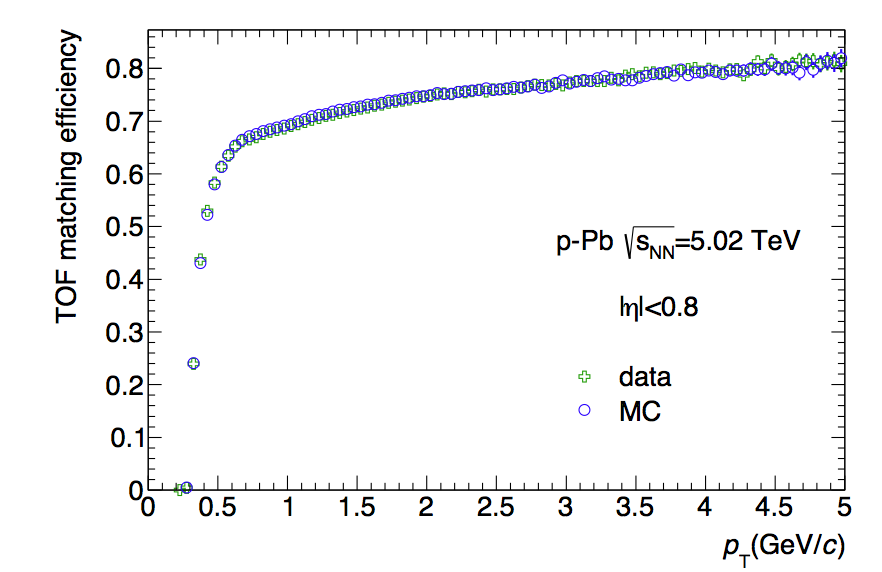
\includegraphics[width=10cm]{chap4/figure/TOF/tofmatcheff.png}
  \caption{Matching efficiency between reconstructed tracks and TOF in p-Pb collisions~\cite{bib_aprrun1}. }
  \label{fig_4_tofmatch}
\end{figure}
TRD also provides a good electron/pion separation above 1 GeV/$c$ but only 12 sectors out of 18 sectors are installed in Run1. 
Therefore, in this analysis, only $dE/dx$ information of TPC is used for electron identification to obtain enough acceptance and detection efficiency. 

TPC $dE/dx$ obeys the Bethe-Bloch formula as described in Section~\ref{sec_3_pid}. 
The ALEPH TPC introduced the useful parametrization to match of the Bethe-Bloch curve in real data. 
The expected dE/dx value is approximated by the following equation, 
\begin{equation}
  \langle \cfrac{dE}{dx} \rangle_{expected} = f(\beta \gamma) = \cfrac{P_{1}}{\beta^{P_{4}}}\big( P2-\beta^{P_{4}}-ln(P_{3}+\cfrac{1}{(\beta\gamma)^{P5}}) \bigr)
\end{equation}
where {$\rm{P_{1}, P_{2}, P_{3}, P_{4}, ~and~P_{5}}$ are the parameters called as ALEPH parameters. 
ALEPH parameters are obtained by fitting to momentum dependent TPC $dE/dx$ distribution of the experimental data.
Since the truncated mean distribution can be described by gaussian, TPC n$\sigma_{ele}$ which expresses the difference from the mean point of electrons is also calculated by 
\begin{equation}
  \rm{TPC~n}\sigma_{\rm{ele}} = \cfrac{\cfrac{\it{dE}}{\it{dx}}_{\rm{measured}} - \langle \cfrac{\it{dE}}{\it{dx}} \rangle_{\rm{expected}} }{\sigma_{\rm{ele}}}
\end{equation}

\subsection{Additional Calibration of TPC PID Using Conversion Electrons}
\label{sec_4_convpid}
For the data driven quality assurance of electron identification, conversion electrons are very useful because we can obtain high purity samples of electrons with the V0-finder.
V0-finder is used for the reconstruction of secondary decay vertices like $\Lambda$, $K^{0}_{s}$, and $\gamma$. 
Figure~\ref{fig_4_v0finder} shows the schematics of the V0 reconstruction. 
V0-finder calculates the pair DCA for all unlike-sign pairs whose leg tracks have large impact parameters and find the secondary decay pairs during track reconstruction. 
\begin{figure}[!h]
  \centering
  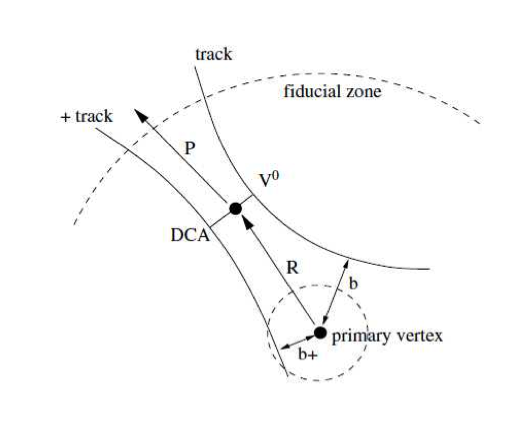
\includegraphics[width=8cm]{chap4/figure/PID/v0-finder.eps}
  \caption{Schematics of V0-finder. }
  \label{fig_4_v0finder}
\end{figure}

Since conversion electrons are produced from real photons in the detectors or beam pipes, their pair invariant mass is zero (very small opening angle) and they pass through the detectors in the constant magnetic field.  
The left panel of Fig.~\ref{fig_4_almenterosandpurity} shows the Almenteros-Podolanski plot in p-Pb collisions.
The x-axis is defined as longitudinal momentum asymmetry. 
The y-axis $q_{T}$, which is defined as projection of the momentum of daughters with respective to the mother $p_{T}$ direction ($\it{p}\times \rm{sin}\theta_{\rm{mother-daughter}}$). 
Conversion electrons are populated around zero due to the massless photon decays.  
%They also have unique other topological features such as their pair plane angle to the magnetic field. 
The cut setting for finding conversion electrons is summarized in Table.~\ref{table_convcut}.
\begin{table}[!h]
  \centering
  \begin{tabular}{cc} \hline
    Cut  & Value \\ \hline
    V0 status  & On-The-Fly \\ 
    Minimum leg $p_{T}$  & $>$ 0.05 GeV/c \\ 
    TPC $N_{cls}$/$N_{findable}$ & $>$ 0.6 \\ 
    $R_{conv}$  & 5 $<$ R $<$ 180 cm \\
    $Z_{conv}$  & Z $<$ 240 cm \\ 
    $DCA_{pair}$  & $<$ 0.25 cm\\ 
    $\Psi_{pair}$  & $<$ 0.05 \\ 
    $(\alpha/0.95)^{2}~+~(q_{T}/0.05)^{2}$  & $<$ 1 \\ 
    $m_{ee}$  & $<$ 50 MeV/$c^{2}$ \\ \hline
  \end{tabular}  
  \label{table_convcut}
  \caption{Summary of the conversion electron selections. }
\end{table}

Conversion electrons can be selected with high purity $>$ 98\% in all $p_T$ region as shown in the right panel of Fig.~\ref{fig_4_almenterosandpurity}. 
The purity is extracted by the full Monte-Carlo simulation with the minimum bias events from DPMJet generator which reproduces the charged particle multiplicity in p-Pb collisions~\cite{bib_dpmjet}.  
\begin{figure}[!h]
 \begin{minipage}{0.5\hsize}
  \begin{center}
  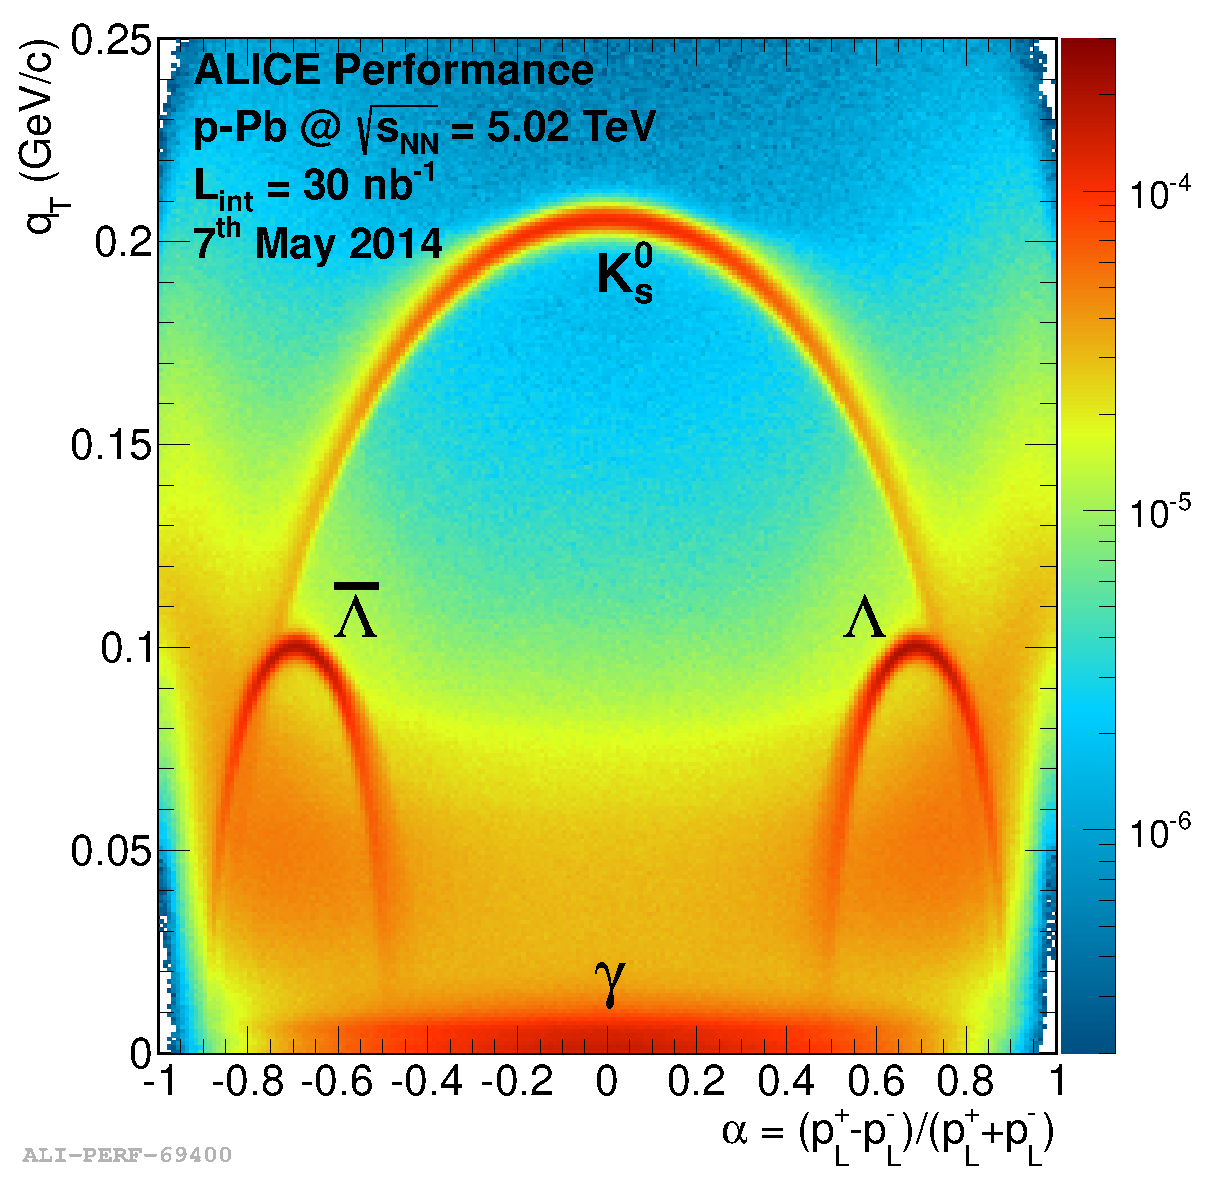
\includegraphics[width=6cm]{chap4/figure/Conversion/ArmenterosPlot_pPb.eps}}
  \end{center}
 \end{minipage}
 \begin{minipage}{0.5\hsize}
  \begin{center}
  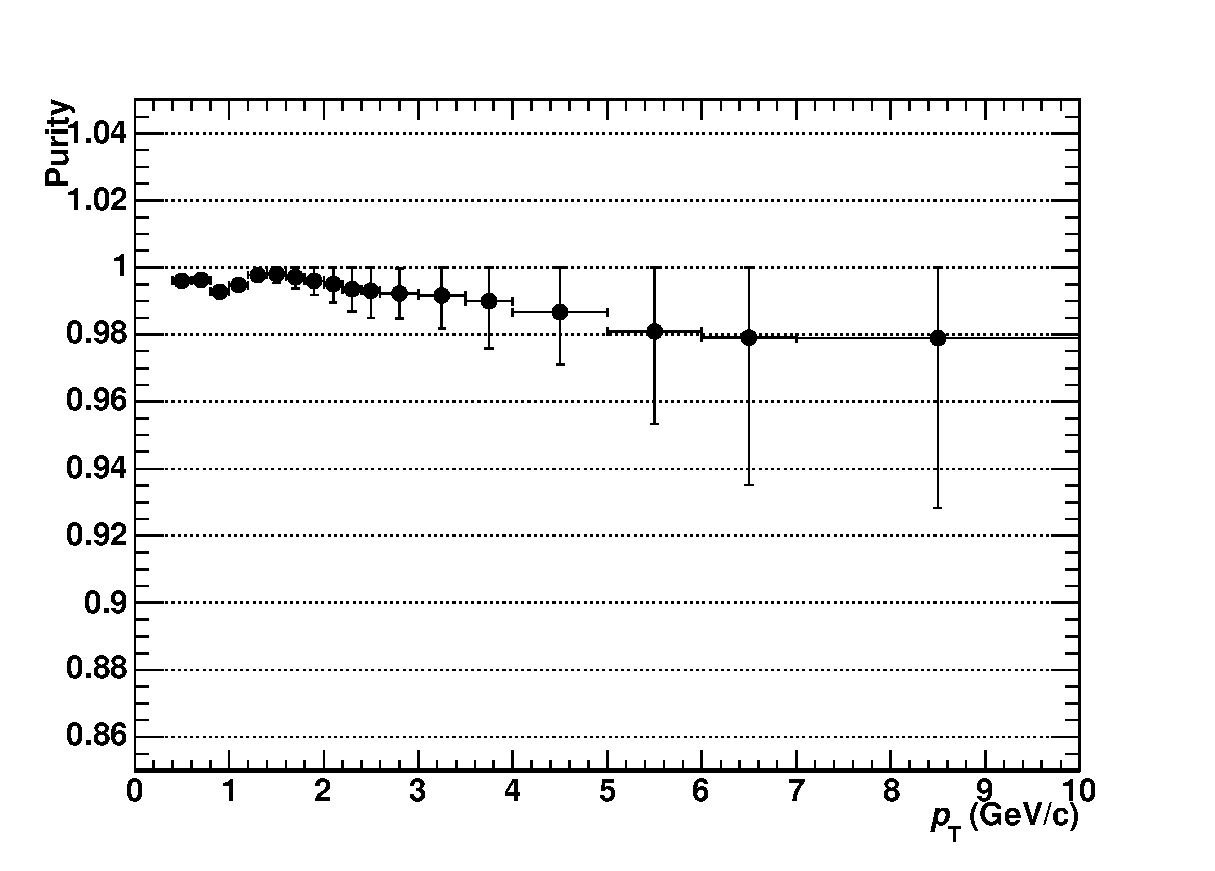
\includegraphics[width=8cm]{chap4/figure/Conversion/SingleV0Cut_ElePurity_Pt.eps}
  \end{center}
 \end{minipage}
  \caption{Almenteros-Podolanski plot in p-Pb collision at $\sqrt{s_{NN}}=$5.02 TeV (Left) and the electron purity of conversion samples extracted by the full Monte-Carlo simulation.  }
  \label{fig_4_almenterosandpurity}
\end{figure}

\begin{figure}[htbp]
 \begin{minipage}{0.5\hsize}
  \begin{center}
  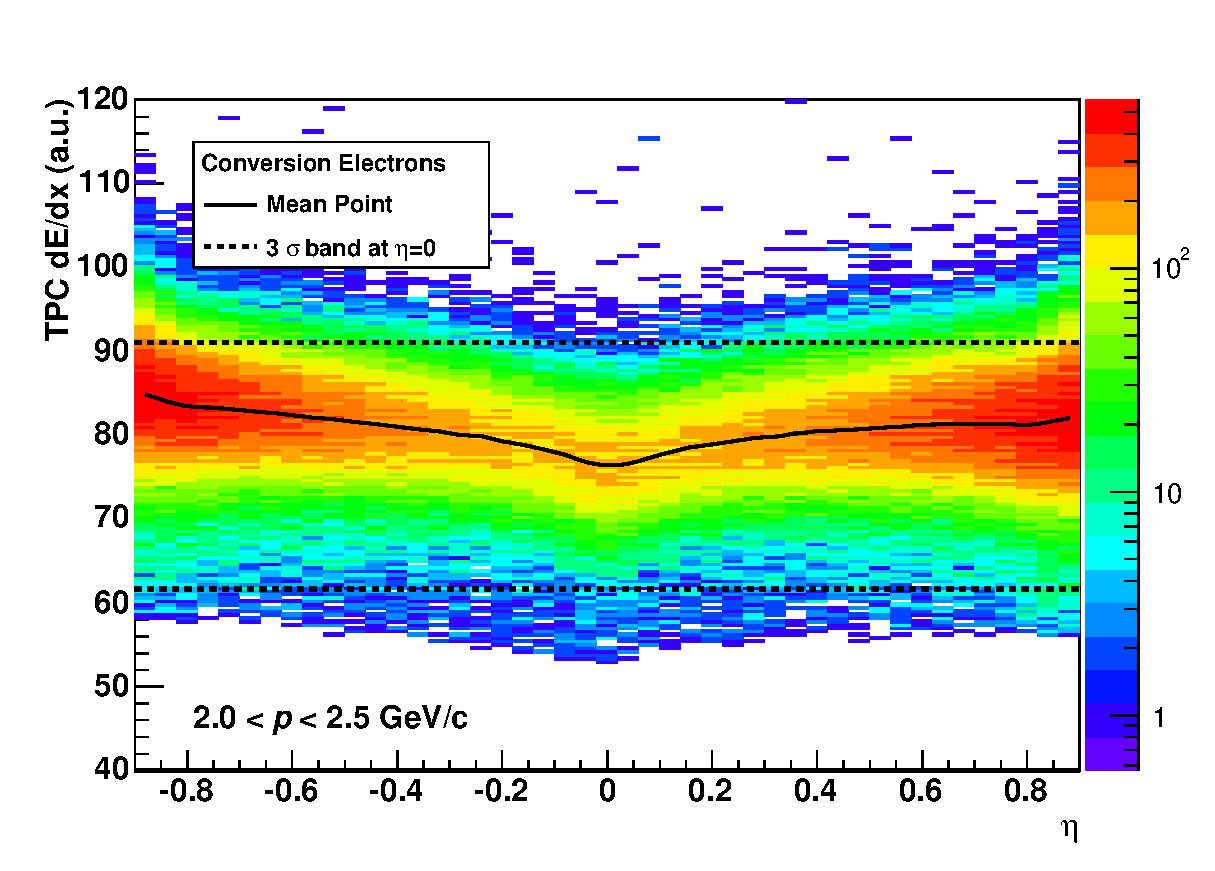
\includegraphics[width=8cm]{chap4/figure/PID/RawTPCdEdxforConv_MB.eps}
  \end{center}
 \end{minipage}
 \begin{minipage}{0.5\hsize}
  \begin{center}
  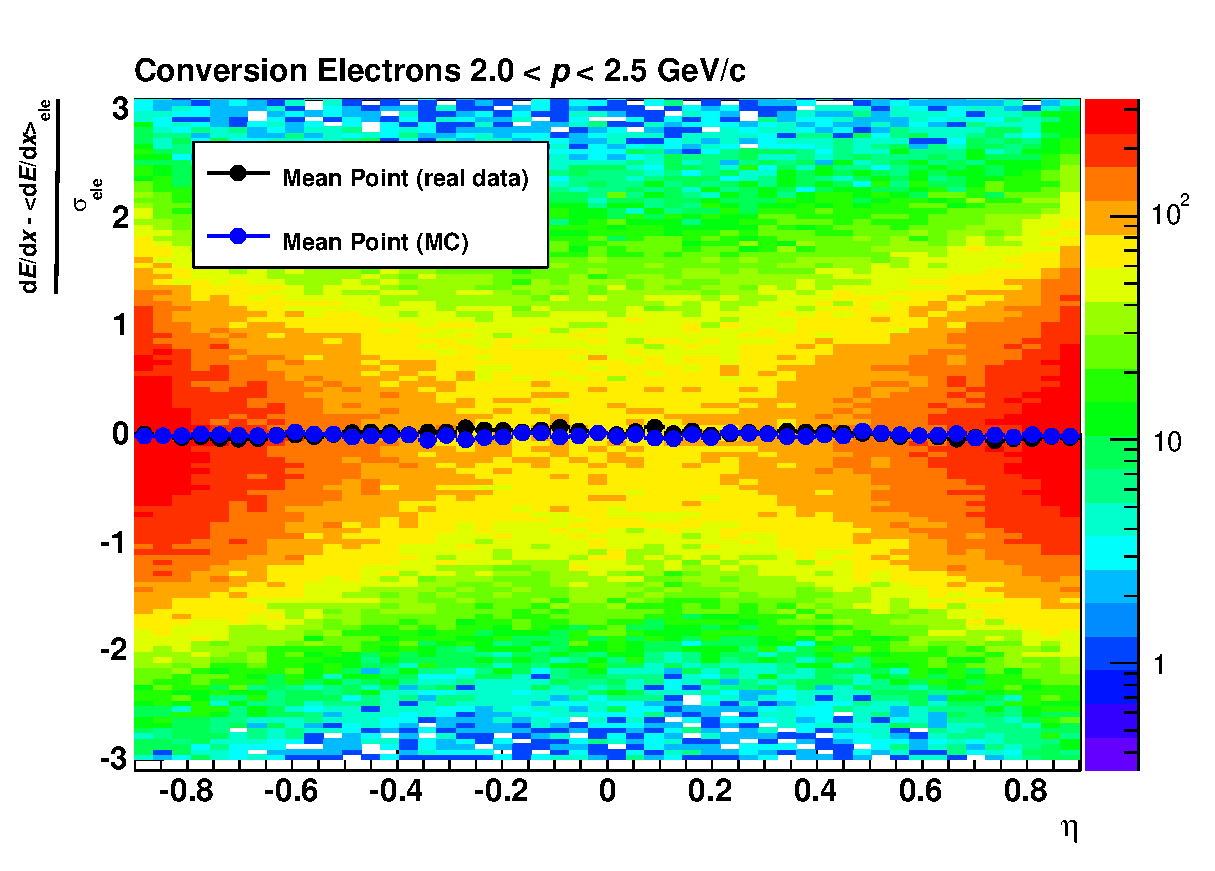
\includegraphics[width=8cm]{chap4/figure/PID/TPCNSigmaforConv_MB.eps}
  \end{center}
 \end{minipage}
  \caption{$\eta$ dependence of the raw TPC dE/dx and the TPC n$\sigma_{\rm{ele}}$ distribution after spline correction for conversion electrons in p-Pb collisions (Left).}
  \label{fig_4_tpcdedxforconv}
\end{figure}

The left panel of Fig.~\ref{fig_4_tpcdedxforconv} shows the $\eta$ dependence of raw TPC $dE/dx$ for conversion electrons. 
Due to the difference of path length, deposited charge distribution has strong $\eta$ dependence. 
In order to treat with the TPC $dE/dx$ values uniformly in the acceptance, 3D-spline ($p_{T}$, $\eta$, $\phi$) function is generated and the corrected TPC $dE/dx$ values are obtained by poisson smearing. 
The right panel of Fig.~\ref{fig_4_tpcdedxforconv} shows the $\eta$ dependence of TPC n$\sigma_{\rm{ele}}$ distribution after 3-D correction.  
The distribution shows the flat shape as a function of $\eta$.  
Figure~\ref{fig_4_tpc_pidfit} shows the quality of the signal shape fitting and the comparison to Monte-Carlo simulation. 
The good agreement between real data and Monte-Carlo simulation as a function of $\it{p}$ is obtained and this Monte-Carlo production is used in the efficiency correction of the electron identification.  
\begin{figure}[!h]
  \centering
  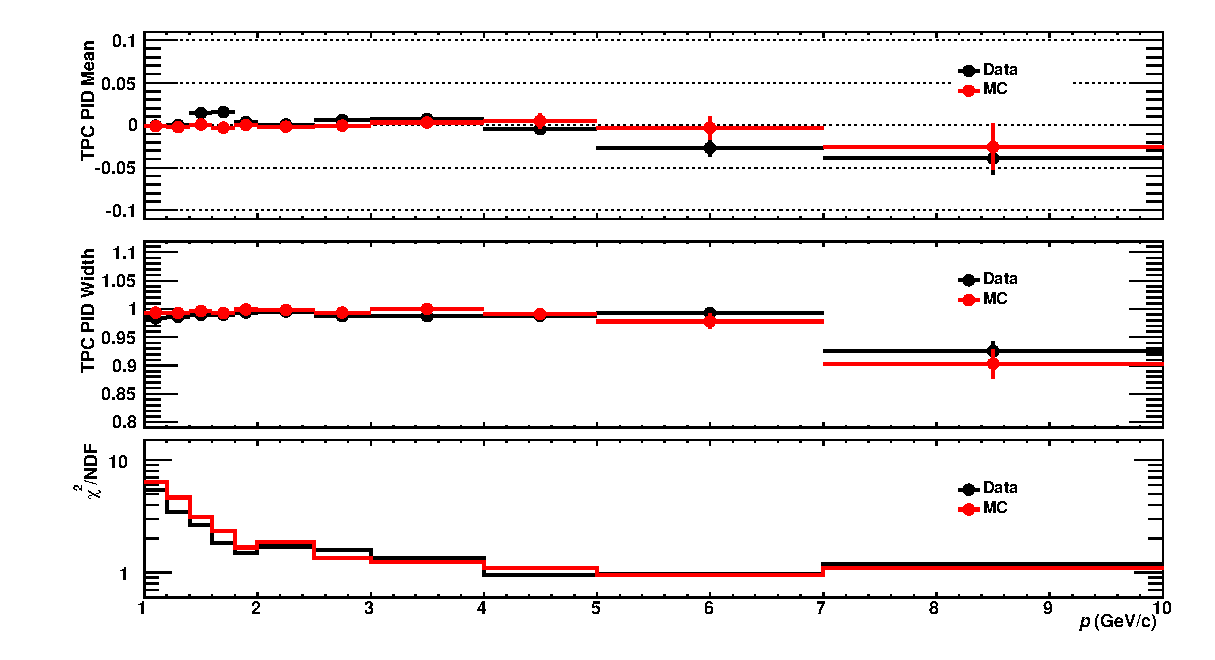
\includegraphics[width=12cm]{chap4/figure/PID/ConvFit_AddEtaCorr_MB.eps}
  \caption{Mean, width, and $\chi^{2}/\rm{NDF}$ of TPC n$\sigma_{\rm{ele}}$ distribution of conversion electrons. The black markers show the results of the analyzed data and the red markers show the results of Monte-Carlo simulation.}
  \label{fig_4_tpc_pidfit}
\end{figure}


\subsection{Cut Setting of TPC PID}
\label{sec_4_cutset}
As a first step of electron identification, all tracks whose TPC $dE/dx$ are within 3$\sigma_{ele}$ are selected. 
The left panel of Fig.~\ref{fig_4_tpcinclusion} shows the TPC n$\sigma_{\rm{ele}}$ distribution within $|\rm{n}\sigma_{\rm{ele}}|<$ 3 as a function of the reconstructed momentum. 
Large hadron contamination exists with only inclusion cut mainly from pions and protons, and deuterons. 
The proton and deuteron band of TPC $dE/dx$ across the electron band around 1 GeV/$c$ and 2 GeV/$c$, respectively.  
Pions distribute the lower side of the Fig.~\ref{fig_4_tpcinclusion} and electron bands start to merge at higher $p_{\rm{T}}$ and hadron contamination extremely increases.   
\begin{figure}[!h]
 \begin{minipage}{0.5\hsize}
  \begin{center}
  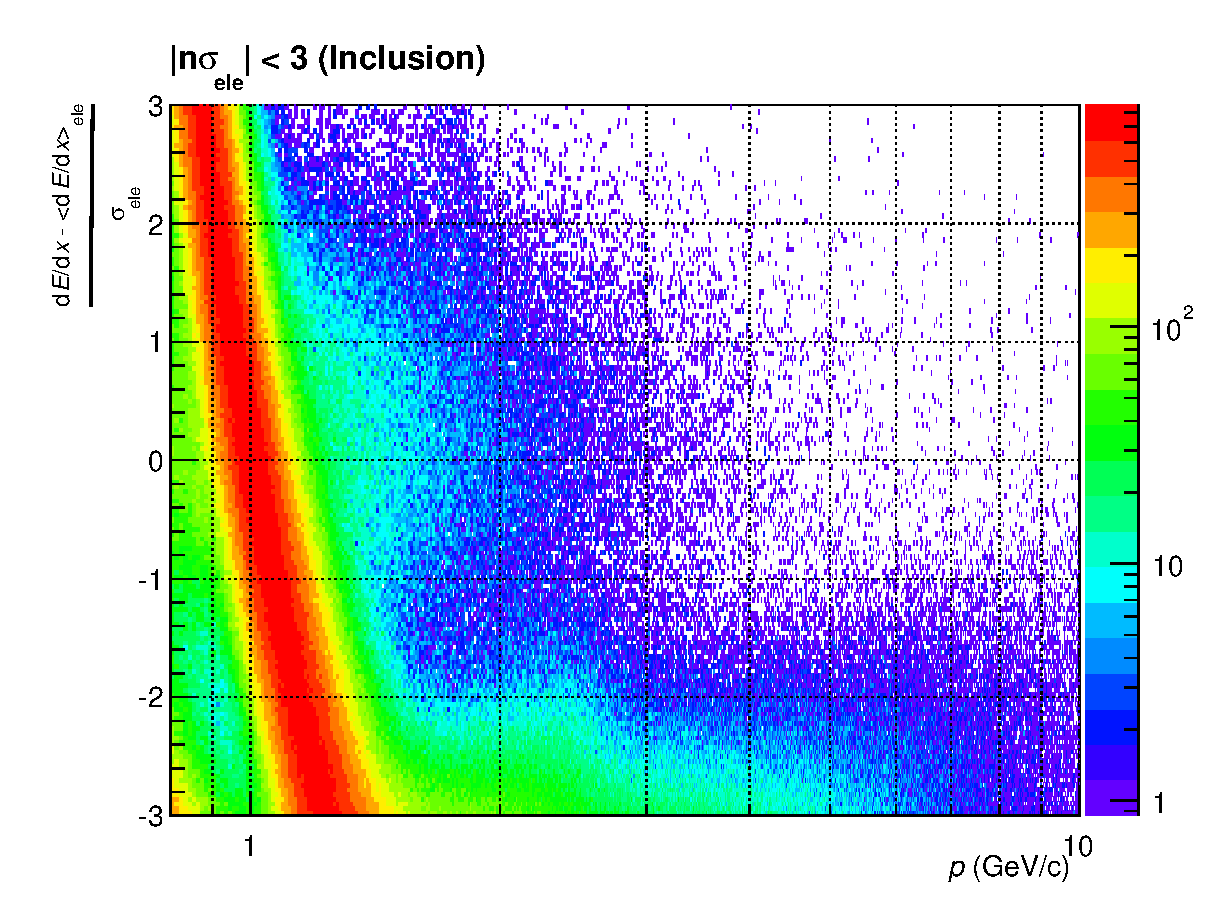
\includegraphics[width=8cm]{chap4/figure/PID/TPCNSigma_AfterInclusion_MB.eps}
  \end{center}
 \end{minipage}
 \begin{minipage}{0.5\hsize}
  \begin{center}
  %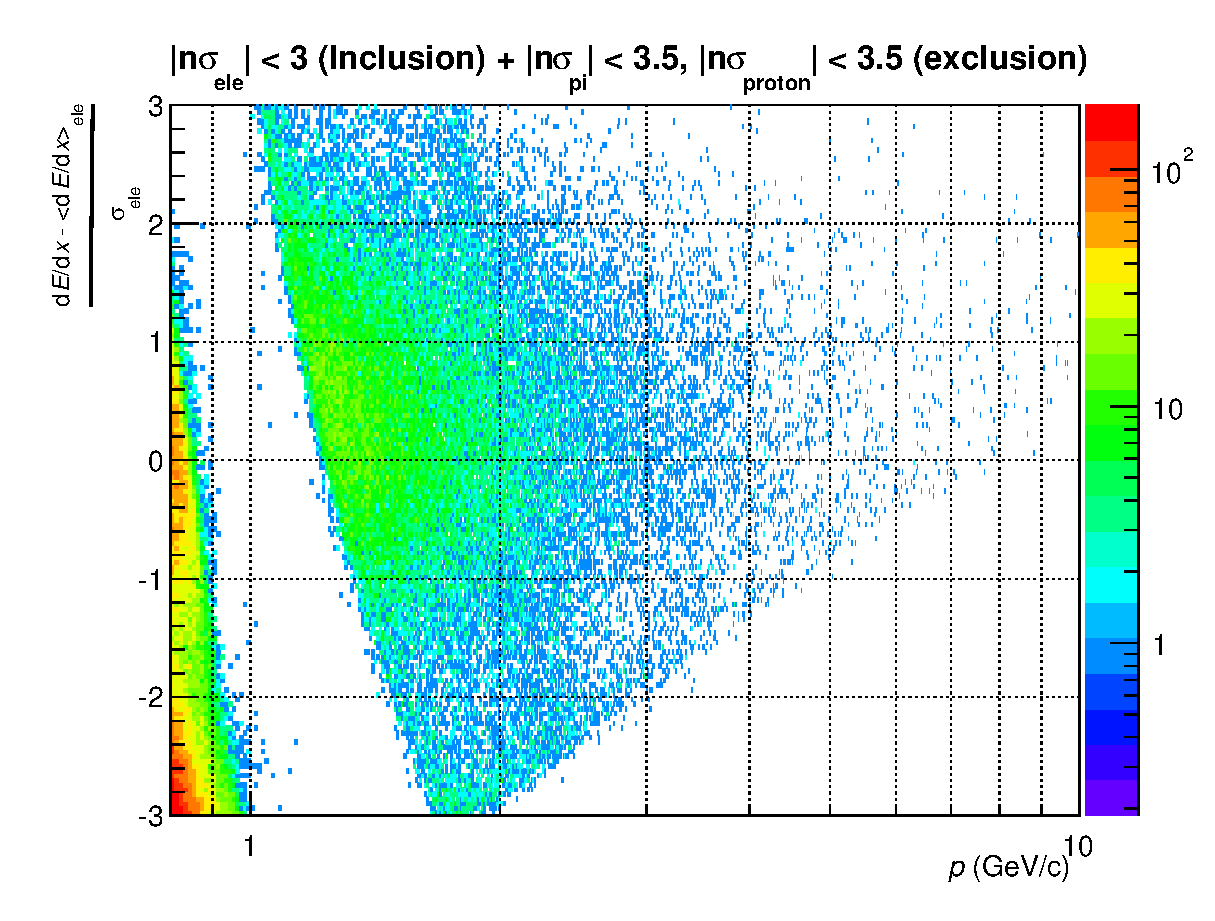
\includegraphics[width=8cm]{chap4/figure/PID/TPCNSigma_AfterExclusion_MB.eps}
%    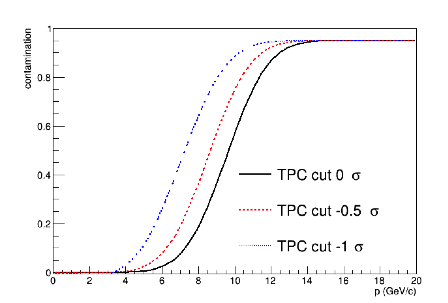
\includegraphics[width=8cm]{chap4/figure/PID/hadroncontami_MB.png}
    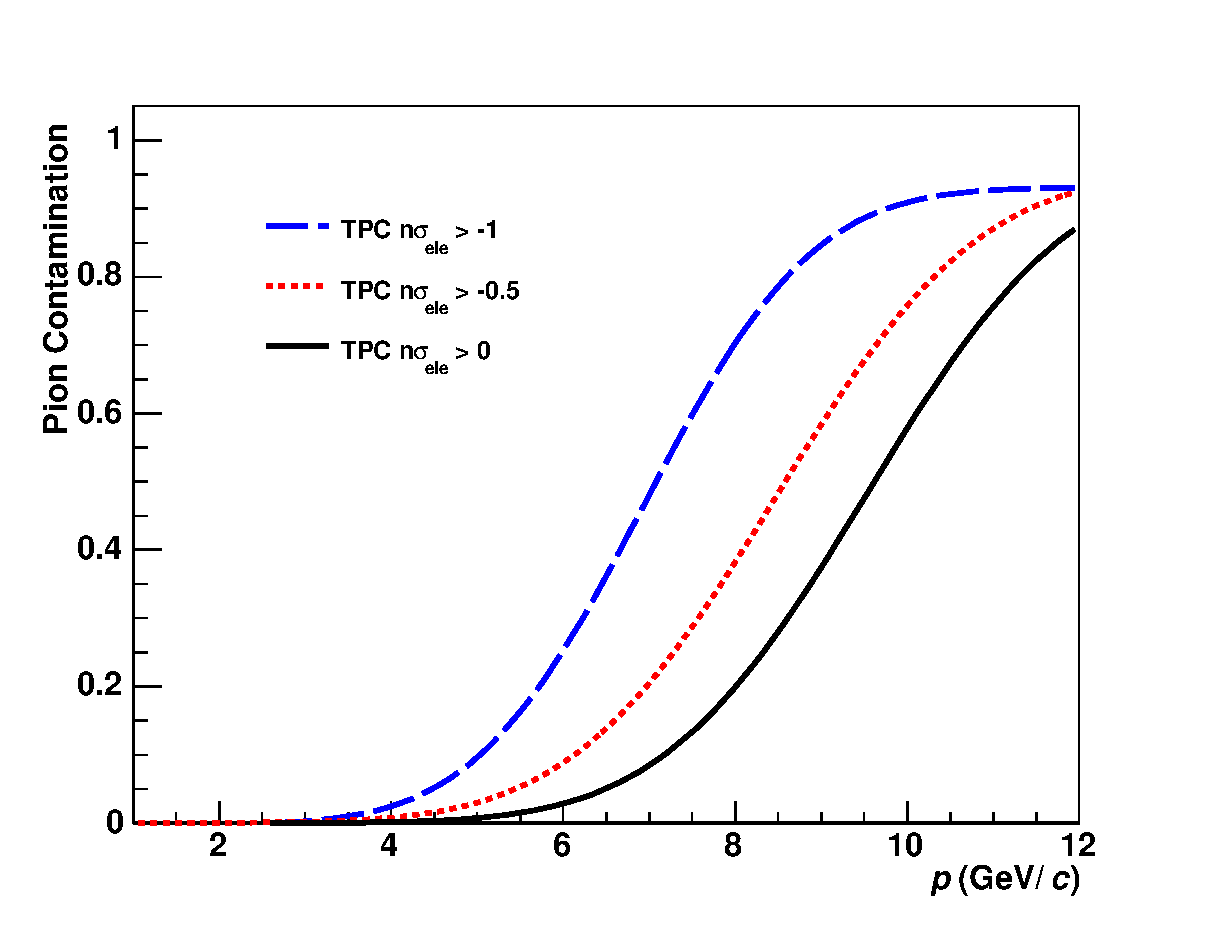
\includegraphics[width=8cm]{chap4/figure/PID/PionContami_MB.eps}
    \end{center}
 \end{minipage}
  \caption{TPC n$\sigma_{\rm{ele}}$ distribution as function of $p$ without hadron exclusion cuts (Left)  and 
	  pion contamination as a function of $p$ with the electron inclusion cut $\sigma_{\rm{ele}}>-1$, $\sigma_{\rm{ele}}>-0.5$, and $\sigma_{\rm{ele}}>0$  (Right) in p-Pb collisions.	
   }
  \label{fig_4_tpcinclusion}
\end{figure}
Figure~\ref{fig_4_tpcinclusion} shows n$\sigma_{ele}$ cut dependence of the pion contamination as a function of $p$. 
The electron and pion contributions are estimated by the fitting of multi-gaussian functions from real data. 
The pion contamination increases rapidly like a step function above the momentum threshold depending on the inclusion cut value.
\begin{figure}[htbp]
 \begin{minipage}{0.5\hsize}
  \begin{center}
  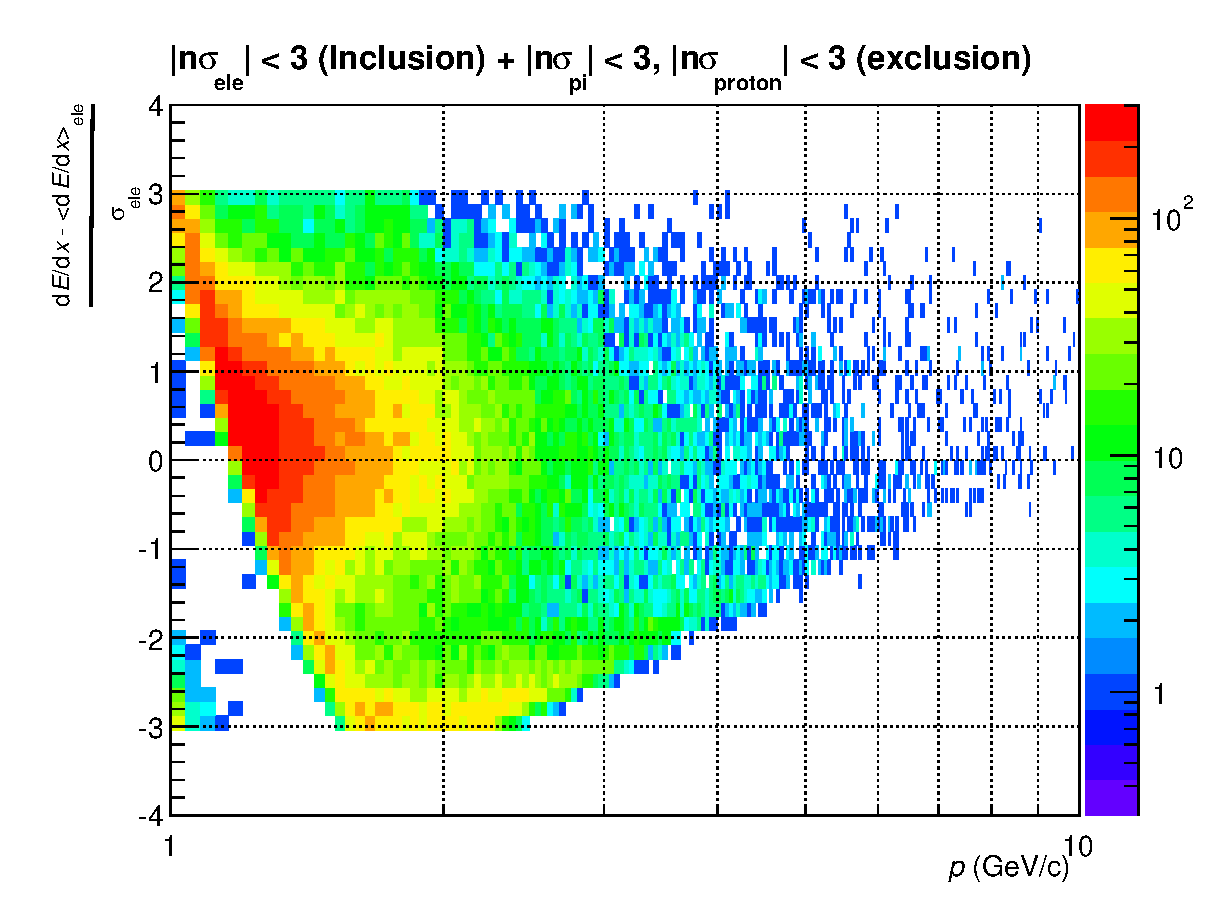
\includegraphics[width=8cm]{chap4/figure/PID/TPCNsigmaElevsp_Selected_ex3.eps}
  \end{center}
 \end{minipage}
 \begin{minipage}{0.5\hsize}
  \begin{center}
  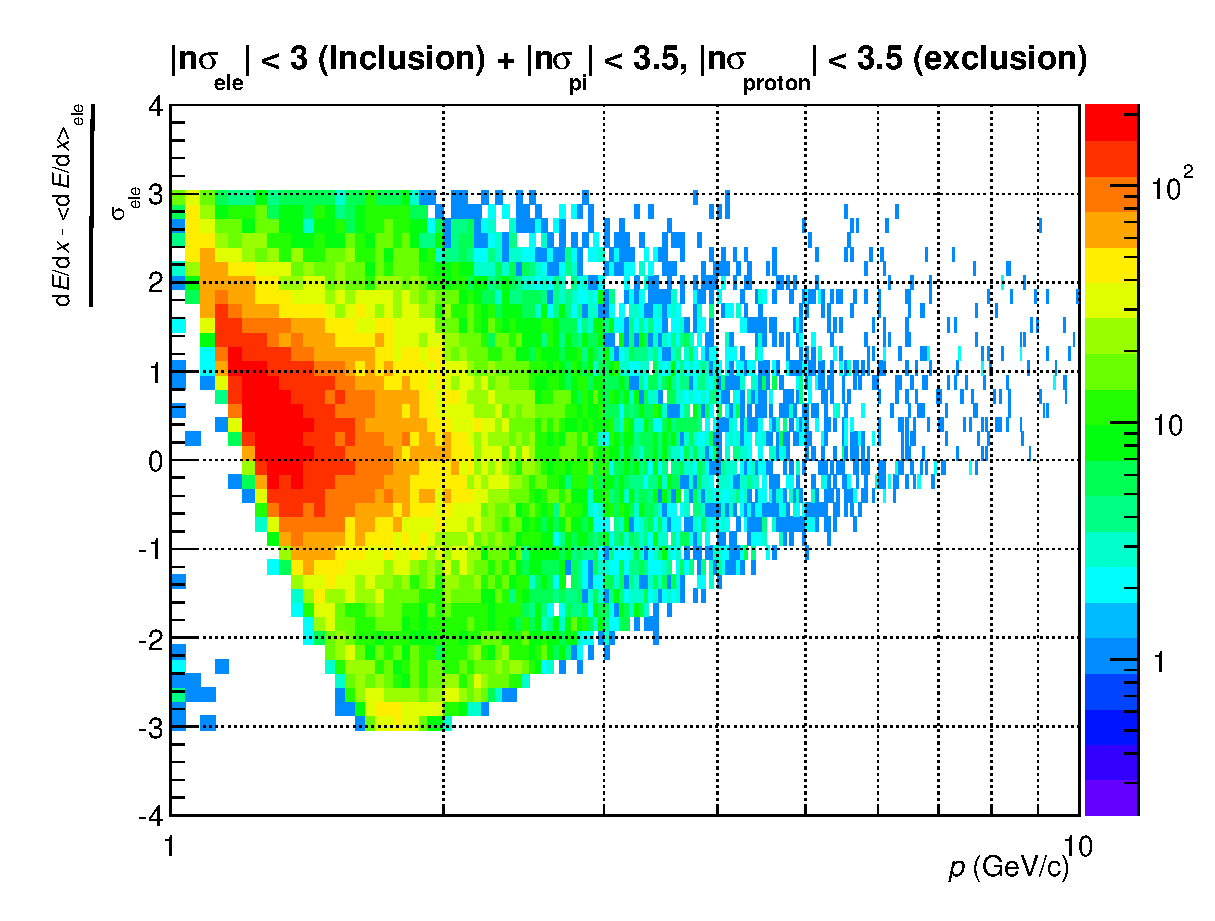
\includegraphics[width=8cm]{chap4/figure/PID/TPCNsigmaElevsp_Selected_ex3p5.eps}
  \end{center}
 \end{minipage}
  \caption{TPC n$\sigma_{ele}$ distribution as function of $p$ with $|\sigma_{\rm{pi}}|<3$ and $|\sigma_{\rm{pro}}|<3$ exclusion cuts (Left) and $|\sigma_{\rm{pi}}|<3.5$ and $|\sigma_{\rm{pro}}|<3.5$ exclusion cuts (Right) in p-Pb collisions.}
  \label{fig_4_tpcnsigmawex}
\end{figure}

To suppress hadron contamination within the acceptable level, pion and proton exclusion cuts are applied. 
TPC $dE/dx$ bands of pions (n$\sigma_{\rm{pi}}$) and protons (n$\sigma_{\rm{pro}}$) are calculated in the same way as TPC n$\sigma_{\rm{ele}}$ with the expected curves of pions and protons.
Figures~\ref{fig_4_tpcnsigmawex} show the TPC n$\sigma_{\rm{ele}}$ applied by pion and proton exclusion cuts. 
There are still non-negligible contribution of pion, proton, and deuteron. 
Hadron contamination is extracted by simultaneous fitting to TPC n$\sigma_{ele}$ distribution with the templates of each contribution. 
The electron template is obtained by conversion electrons and the shape of deuteron contribution is estimated by the full Monte-Carlo simulation. 
Their mean and with are fixed and the magnitudes are only free parameters. 
The fitting is done by electron dominant region (n$\sigma_{\rm{ele}}>$1) and the residual components are considered as proton and pion contributions. 
The examples of template fitting are shown in  Fig.~\ref{fig_4_tpcnsigmacut3} and \ref{fig_4_tpcnsigmacut3p5}. 
\begin{figure}[!h]
 \begin{minipage}{0.5\hsize}
  \begin{center}
 	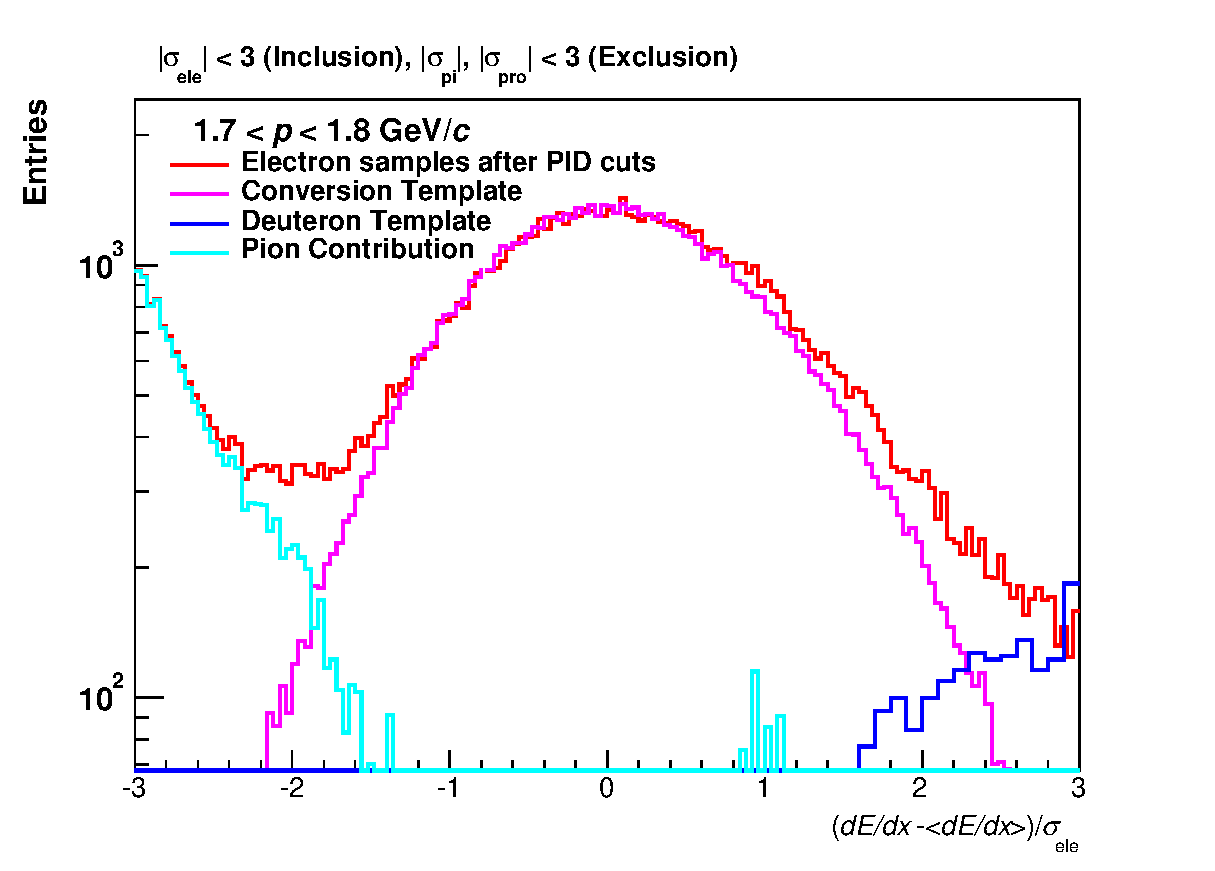
\includegraphics[width=8cm]{chap4/figure/PID/TPCNSigma_AfterExclusion3_MB_1p7_1p8.eps}
  \end{center}
 \end{minipage}
 \begin{minipage}{0.5\hsize}
  \begin{center}
	 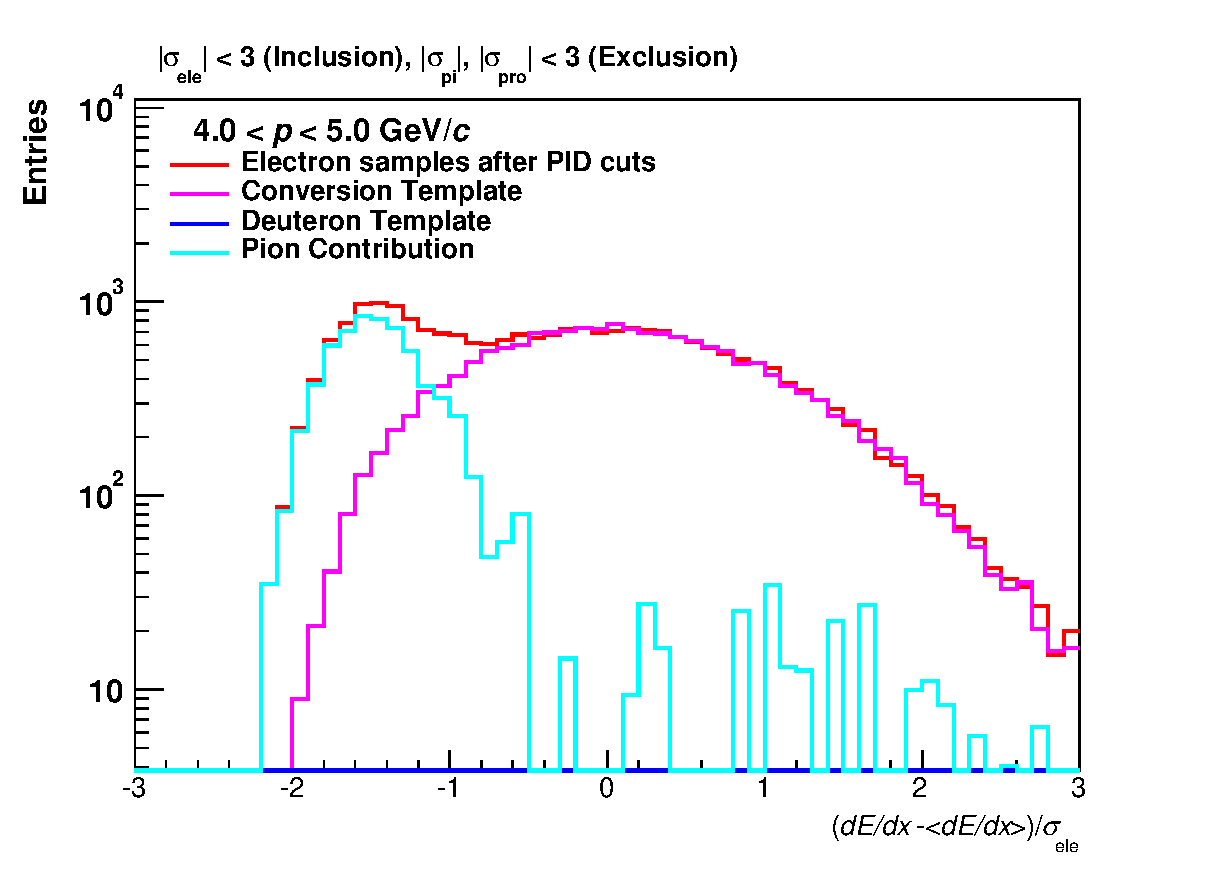
\includegraphics[width=8cm]{chap4/figure/PID/TPCNSigma_AfterExclusion3_MB_4_5.eps}
  \end{center}
 \end{minipage}
  \caption{The template fitting to the TPC n$\sigma_{\rm{ele}}$ distributions in 1.7 $<p<$ 1.8 GeV/$c$ (Left) and 4.0 $<p<$ 5.0 GeV/$c$(Right) with $|\sigma_{\rm{pi}}|<3$ and $|\sigma_{\rm{pro}}|<3$ exclusion cuts.}
  \label{fig_4_tpcnsigmacut3}
\end{figure}
\begin{figure}[!h]
 \begin{minipage}{0.5\hsize}
  \begin{center}
 	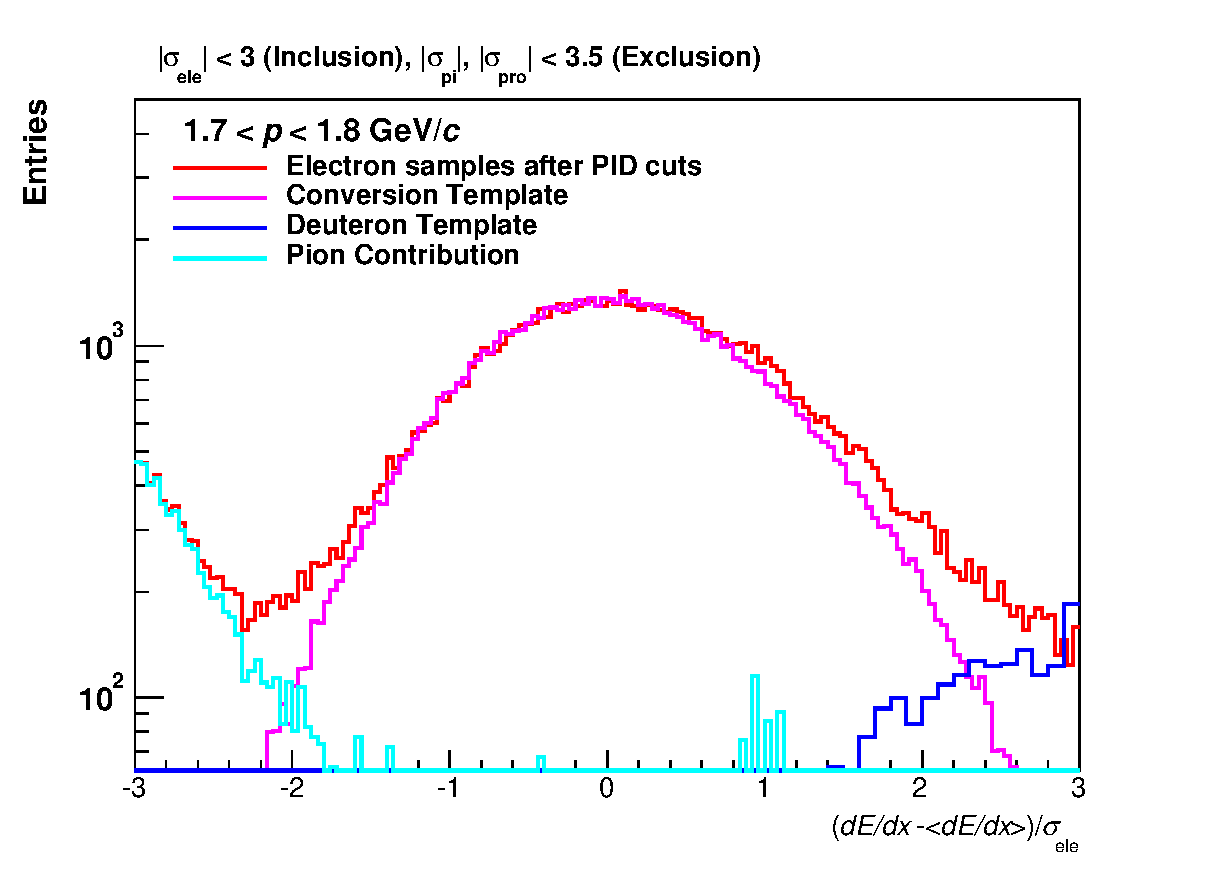
\includegraphics[width=8cm]{chap4/figure/PID/TPCNSigma_AfterExclusion3p5_MB_1p7_1p8.eps}
  \end{center}
 \end{minipage}
 \begin{minipage}{0.5\hsize}
  \begin{center}
	 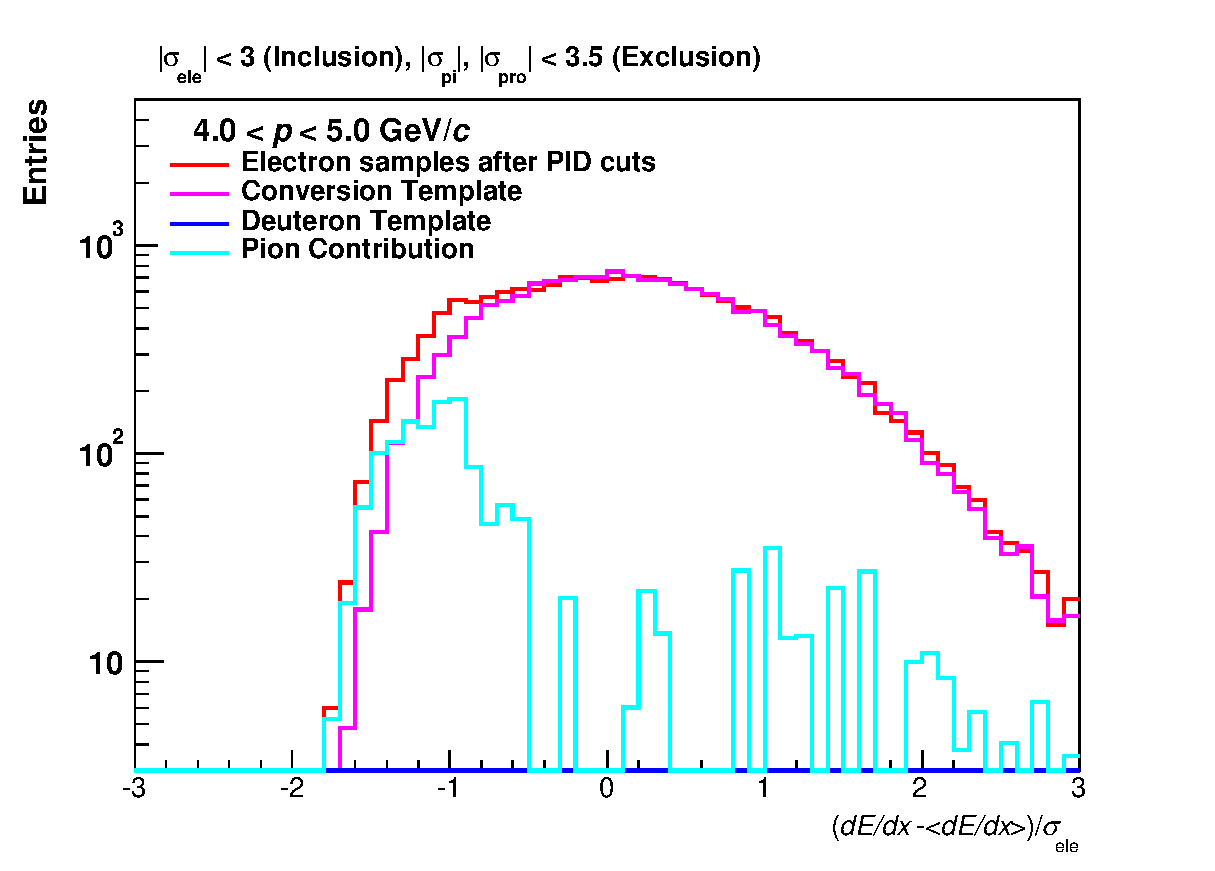
\includegraphics[width=8cm]{chap4/figure/PID/TPCNSigma_AfterExclusion3p5_MB_4_5.eps}
  \end{center}
 \end{minipage}
   \caption{The template fitting to the TPC n$\sigma_{\rm{ele}}$ distributions in $1.7<p<1.8$ GeV/$c$ (Left) and $4.0<p<5.0$GeV/$c$(Right) with $|\sigma_{\rm{pi}}|<$ 3.5 and $|\sigma_{\rm{pro}}| < $ 3.5 exclusion cuts.}
  \label{fig_4_tpcnsigmacut3p5}
\end{figure}

Figure~\ref{fig_4_hadcont}  shows the hadron contamination and single electron identification efficiency as a function of the reconstructed momentum. 
The inclusive hadron contamination is 11\% and the electron samples contains 5\% deuterons, 4\% pions, and 2\% protons. 
Although they contribute to the combinatorial background in the invariant mass distribution of dielectrons, they can be subtracted by the event mixing technique described in the next section. 
And then it is acceptable for the signal extraction of $J/\psi$ signals. 
\begin{figure}[!h]
  \centering
  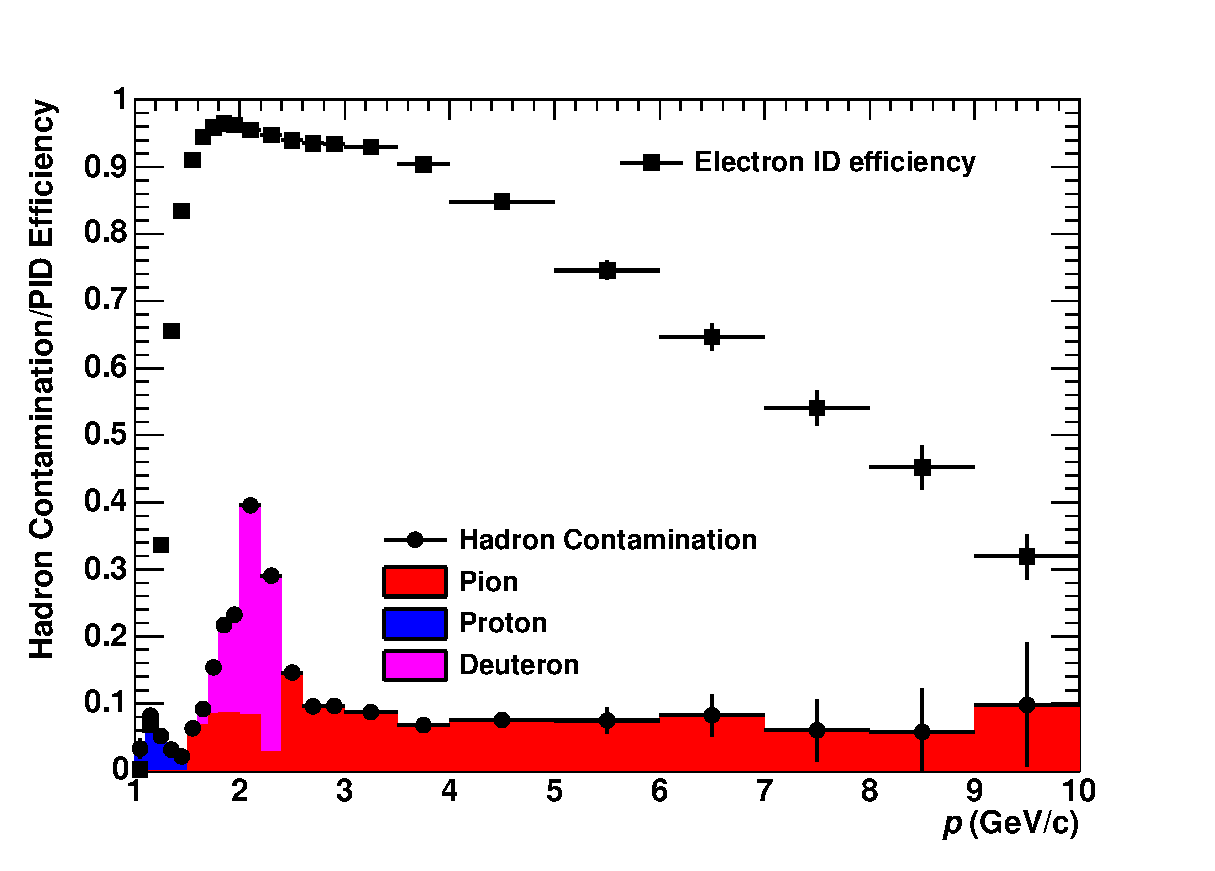
\includegraphics[width=10cm]{chap4/figure/PID/PIDEffvsHadCont_MB_3p5.eps}
  \caption{Single Electron PID efficiency and hadron contamination with pion and proton exclusion cuts in p-Pb collisions at $\sqrt{s_{NN}}=$5.02 TeV.}
  \label{fig_4_hadcont}
\end{figure}

%\subsection{Cut Optimization of Track Cuts and Electron Identification Cut}
The main parameters to be optimized of $J/\psi$ signal extraction are SPD hit requirement and TPC electron identification cuts. 
The all combination of the following cut setting are checked. 
\begin{description}
\item{leg $p_{\rm{T}}$:} 0.8, 1.0, 1.1 GeV/$c$ \\
\item{SPD hit:} Any, First \\
\item{TPC n$|\sigma_{\rm{pi}}|$ (exclusion):} 2.5, 3, 3.5, 4 \\ 
\item{TPC n$|\sigma_{\rm{pro}}|$ (exclusion):} 3, 3.5, 4  
\end{description}
Figure~\ref{fig_4_cutopt} shows the signal to background ratio, significance, and $\chi^{2}/$NDF of the fitting to the reconstructed $J/\psi$ signals in each $p_{\rm{T}}$ bin with the above cut variation. 
The signal extraction of the $J/\psi$ signals is described in the Section~\ref{sec_4_signalextraction}.
The cut index is summarized in Appendix~\ref{app_b_cutindex}.
%72 combinations of cut parameters are checked and the final cut setting is determined to maximize the significance of $J/\psi$. 
%%Qualitatively, the cut setting of lower $p_{T}$ bins are tuned to increase the signal to background ratio. 
In the lowest $p_{\rm{T}}$ bin, the significance correlates the signal to background ratio clearly and SPD First hit requirement improves the signal to background ratio.  
On the other hand, looser cuts show higher significance as $p_{\rm{T}}$ increases since the significance depends on the number of signals more strongly. 
\begin{figure}
\begin{center}
	\subfloat{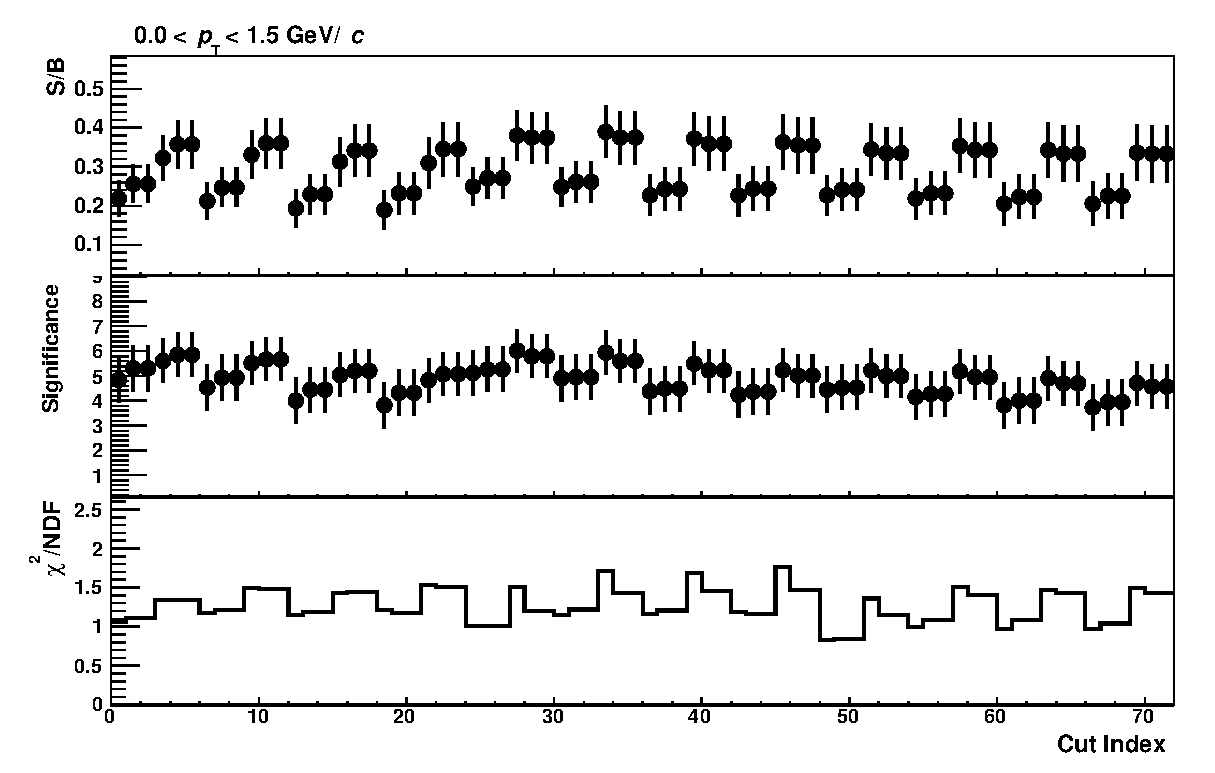
\includegraphics[width=7cm]{chap4/figure/PID/CutOpt/SBSigChi2_MixFit_INT7_MB_0.eps}} \hspace{2mm}
	\subfloat{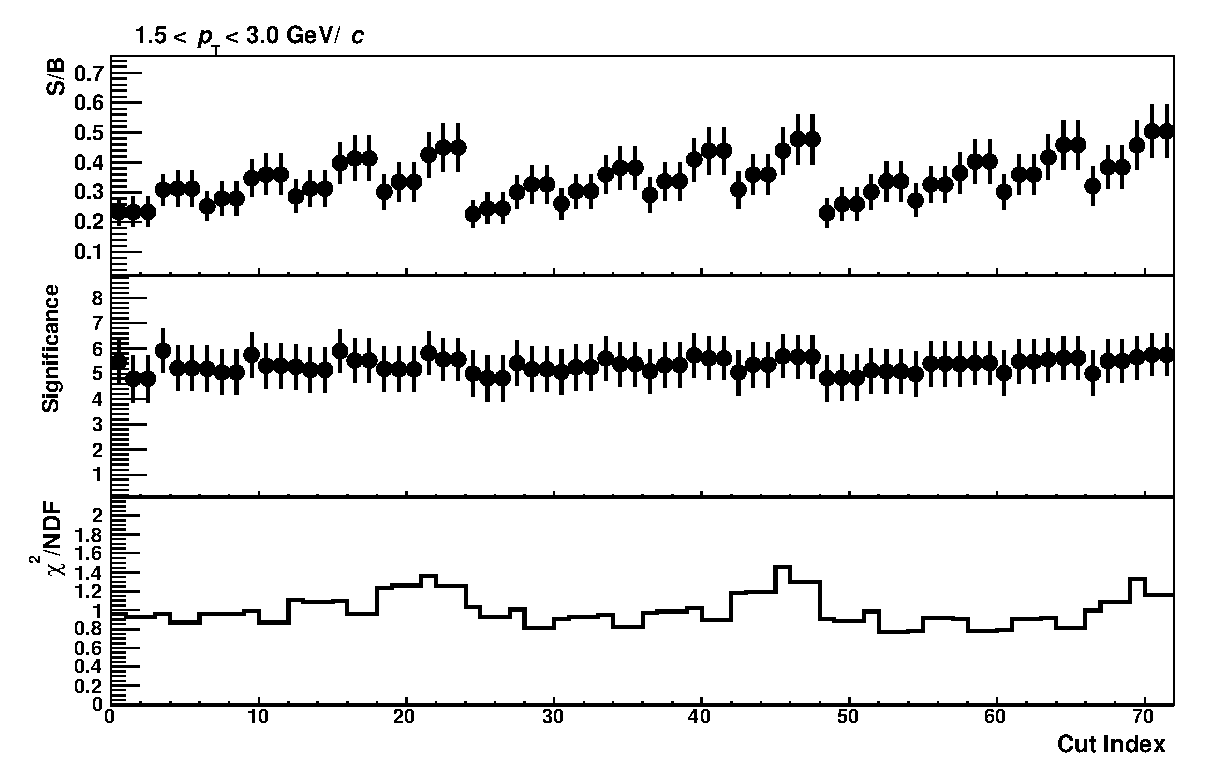
\includegraphics[width=7cm]{chap4/figure/PID/CutOpt/SBSigChi2_MixFit_INT7_MB_1.eps}} \\
	\vspace{1cm}
	\subfloat{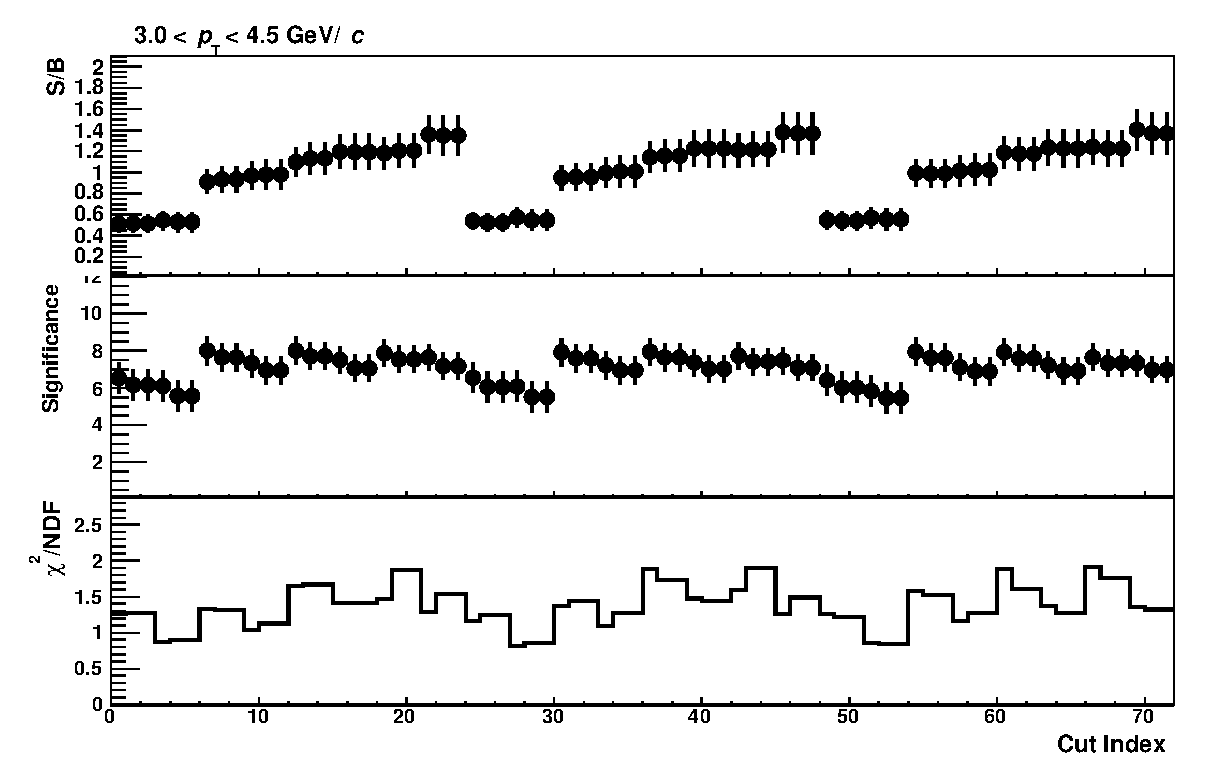
\includegraphics[width=7cm]{chap4/figure/PID/CutOpt/SBSigChi2_MixFit_INT7_MB_2.eps}} \hspace{2mm}
	\subfloat{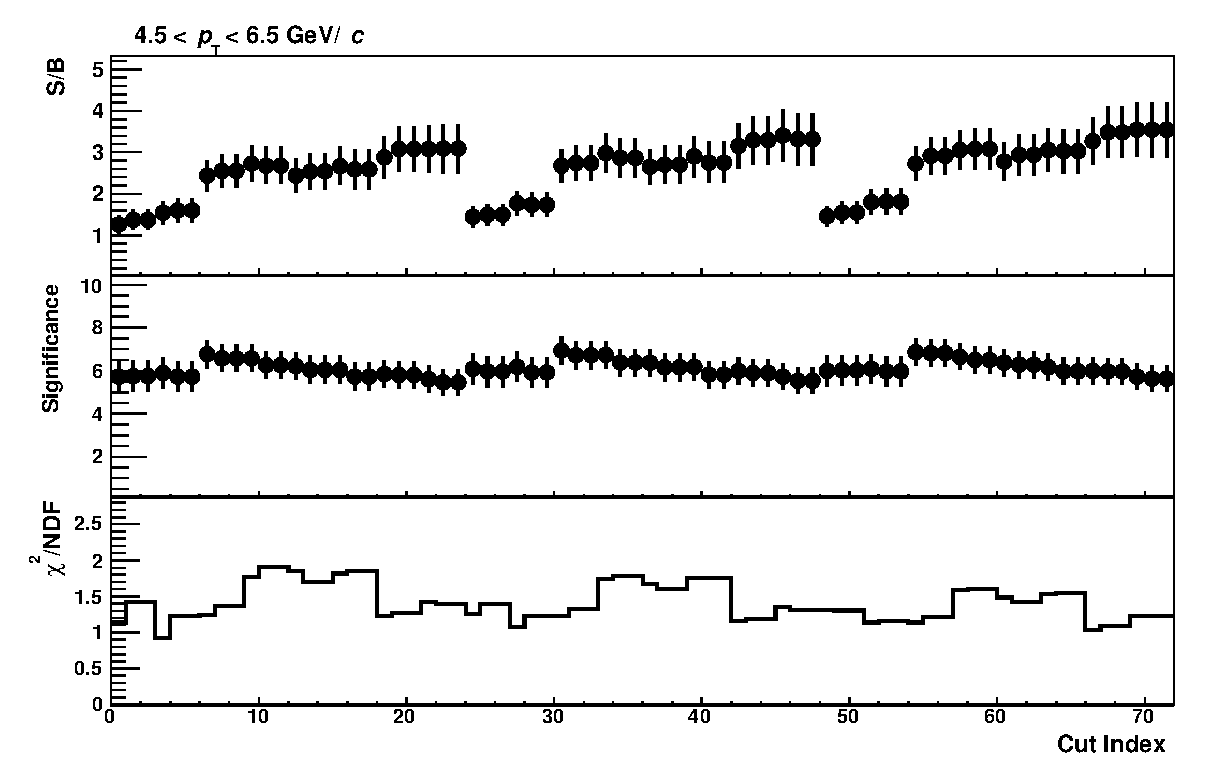
\includegraphics[width=7cm]{chap4/figure/PID/CutOpt/SBSigChi2_MixFit_INT7_MB_3.eps}} \\
	\vspace{1cm}
	\subfloat{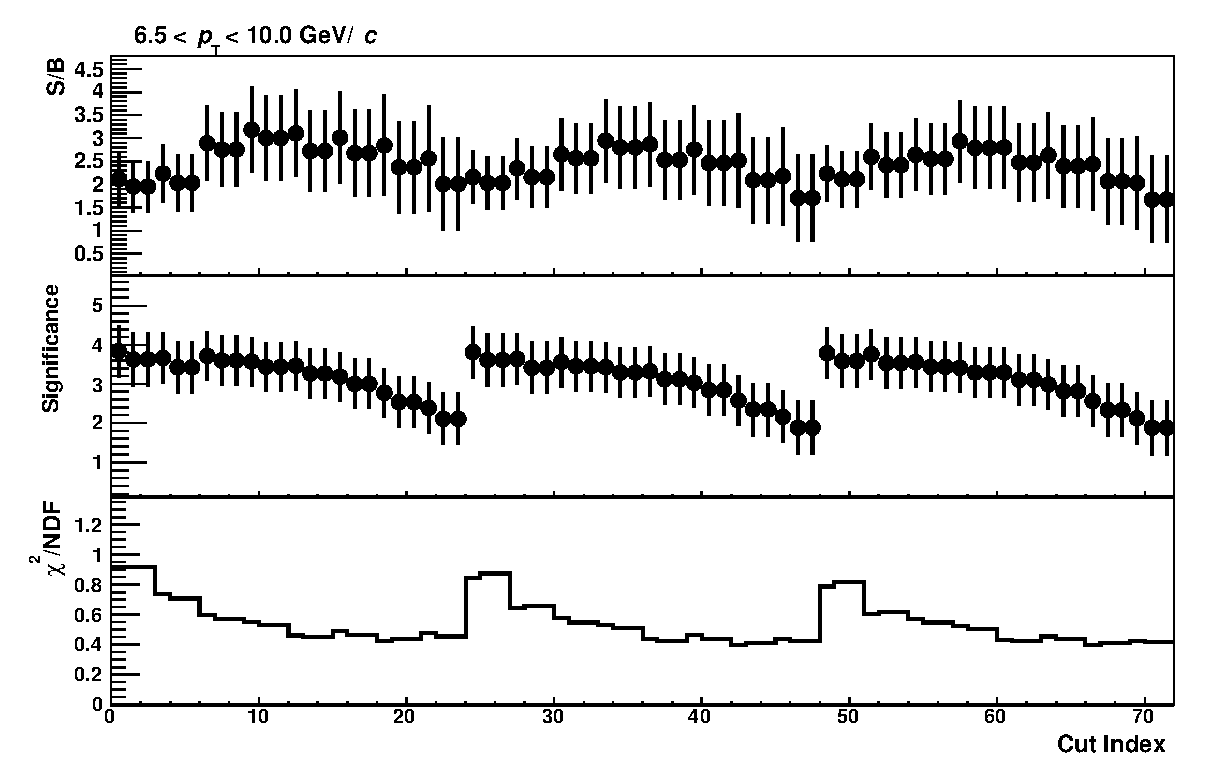
\includegraphics[width=7cm]{chap4/figure/PID/CutOpt/SBSigChi2_MixFit_INT7_MB_4.eps}} 
\end{center}
\caption{Signal to background ratio, significance, and $\chi^{2}/$NDF of the fitting to the reconstructed $J/\psi$ signals in each $p_{\rm{T}}$ bin.  The cut index is summarized in Appendix~\ref{app_b_cutindex}.  }
\label{fig_4_cutopt}
\end{figure}

Table~\ref{table_4_cutset} shows the summary of the leg $p_{\rm{T}}$, SPD hit and TPC PID cut setting.
Figure~\ref{fig_4_singleeff} shows the electron identification efficiency of single electrons as a function of the reconstructed momentum . 
Good agreement between data and Monte-Carlo simulation is seen. 
\begin{table}[!h]
  \centering
    \begin{tabular}{ccccc} \hline
      $p_{T}$ bin (GeV/c)  & $p^{e}_{T}$ cutoff (GeV/c) & SPD hit & TPC n$\sigma_{pion}$ & TPC n$\sigma_{proton}$\\ \hline
      0-1.5                &  1.0  & First   &     3.0                           & 3.5                                      \\ 
      1.5-3.0              & 1.0  & First   &     3.5                          & 3.5                                      \\ 
      3.0-4.5              & 0.8  & Any     &     3.0                           & 3.5                                      \\ 
      4.5-6.5              & 0.8  & Any     &     3.0                           & 3.5                                      \\ 
      6.5-10.0             & 1.0  & Any     &     3.0                           & 3.0                                      \\  \hline
    \end{tabular}
    \caption{Summary of the cut parameters.}
    	\label{table_4_cutset}
\end{table}

\begin{figure}[!h]
  \begin{center}
    %\includegraphics[width=12cm]{chap4/figure/PID/SinglePIDEff_LHC13d10.eps}
    \includegraphics[width=10cm]{chap4/figure/PID/SinglePIDEfficinecy_DatatoMC_LHC13b2efix.eps}
  \end{center}
  \caption{Hadron exclusion cut dependence of single electron identification efficiency (Upper) and ratio of data to MC (Lower) in p-Pb collisions.}
  \label{fig_4_singleeff}
\end{figure}
Figure~\ref{fig_4_singleeff} shows single electron identification efficiency as a function of reconstructed momentum for conversion electrons in Data and MC. 
%At low $p_{\rm{T}}$, there is the non-negligible deviation between data and MC due to the difference of TPC n$\sigma_{pro}$ distributions. 
%The mean point and width of electrons are identical within the uncertainty in Data and MC and the discrepancy doesn\rq{}t show the exclusion cut dependence.  
%The discrepancy is corrected by the ratio as a function of reconstructed momentum in pair efficiency calculation. 

\section{Rejection of Conversion Electrons}
\label{sec_4_convref}
Conversion electrons are main source of electron candidates in all $p_{\rm{T}}$ region.
Hit on the most inner detector (SPD) significantly decrease conversion rejection generated at larger radii than SPD.
However, they still account for 25\% of selected electrons at $p_{\rm{T}} =$ 2 GeV/$c$ as shown in Fig.~\ref{fig_4_single}.  
V0-finder described in Section~\ref{sec_4_convpid} is powerful tool for conversion tagging. 
Monte-Carlo simulation confirms V0-finder reject conversion electrons by a factor of 70\% without any lack of signal electrons. 
Figure~\ref{fig_4_v0tag} shows the unlike-sign pairs and background estimated by event mixing technique described in Section  \ref{sec_4_signalextraction} as a function of the invariant mass with the loose and the tight cuts for the analyzed data before and after the V0-finder cut.
At the $J/\psi$ mass, signal to background ratio is improved by a factor 50\% with V0-finder cut. 
\begin{figure}[htbp]
 \begin{minipage}{0.5\hsize}
  \begin{center}
  \includegraphics[width=8cm]{chap4/figure/V0tag/V0tagCheck_MB_cut7.eps}
  \end{center}
 \end{minipage}
 \begin{minipage}{0.5\hsize}
  \begin{center}
  \includegraphics[width=8cm]{chap4/figure/V0tag/V0tagCheck_MB_cut40.eps}
  \end{center}
 \end{minipage}
  \caption{V0-finder cut dependence of unlike-sign pairs and background spectra estimated by event mixing technique as a function of the invariant mass with the loose cut (SPD any, $|\rm{n}\sigma_{ele}|<3$, $|\rm{n}\sigma_{pi}|<3$, $|\rm{n}\sigma_{pi}|<3$) (Left) and the tight (SPD first, $|\rm{n}\sigma_{ele}|<3$, $|\rm{n}\sigma_{pi}|<3.5$, $|\rm{n}\sigma_{pi}|<3.5$) (Right).  }
  \label{fig_4_v0tag}
\end{figure}

\section{Signal Extraction}
\label{sec_4_signalextraction}
The invariant mass is calculated for all electron-positron pairs. 
The background subtraction is crucial part for the precision of raw yield extraction.  

\subsection{Background Subtraction}
\label{sec_4_bgsub}
The unlike-sign pairs around $J/\psi$ pairs contain the following contributions, 
\begin{description}
\item{-} $J/\psi$ signal
\item{-} Correlated $c\bar{c}$ and $b\bar{b}$ decay pairs
\item{-} Combinatorial pairs, where both electrons and positrons are totally uncorrelated. 
\item{-} Correlated pairs from same or back-to-back jet cone
\end{description}
The main source of the background is combinatorial pairs. 
Event mixing technique is used to estimate the shape of the combinatorial background since this method does not suffer from the statistical limitation by mixing as many events as possible.
The procedure of event mixing is as follows.
\begin{enumerate}
  \item 
  	The events which contain electron candidates are stored in the event pools. 
	The event pools are classified according to the collision vertex and centrality (multiplicity) as below to suppress the event bias. 
	\begin{description}
	  \centering
	   \item[] $\rm{Z_{vtx}}$~(cm) &  $=$ & \{-10, -7.5, -5, -2.5, 0, 2.5, 5, 7.5, 10\}      
	   \item[] \rm{V0M}~\rm{Centrality}~(\%) & $=$ & \{0-20, 20-40, 40-60, 60-80, 80-100\} 
	\end{description}
	If each event pool accumulates a certain number of events called as depth, the mixing events are generated.
	The depth of the event pool in this analysis is 10. 
  \item 
  	The invariant mass and pair $p_{\rm{T}}$ are calculated for all combinations of selected tracks stored in the corresponding event pool except for the same event pairs. 
  \item After event mixing, the corresponding event pool which is used in procedure 2 is cleaned up (delete all stored events) and the next event processing start following procedure 1 again. 
 \end{enumerate}



Like-sign pairs in same events include not only combinatorial background but also correlated background like jet pairs, and bottom pair decays. 
Therefore more reasonable shape of the background can be obtained compared to event mixing technique. 
Figure~\ref{fig_4_lsmix} shows the comparison of the shapes between like-sign method and event mixing technique.
%\begin{eqnarray}
%%\end{eqnarray}
where V0M means the centrality of collisions calculated with the sum of the multiplicities of both V0A and V0C. 
Electrons and positrons from different events are paired in within the same event categories. 
Both of like-sign and event mixing pairs are normalized by the side-band yield of unlike-sign pairs (2-2.5, 3.2-3.7 GeV/$c^{2}$).
The background by like-sign and mixed like-sign pairs show the good agreement within 20\% which comes from the statistics of like-sign pairs.
This also means that the uncorrelated combinatorial pairs are dominant and correlated pairs from jets and bottom quarks are not relevant compared to the statistical uncertainty.
\begin{figure}[!h]
  \centering
  \includegraphics[width=10cm]{chap4/figure/SignalExtraction/BGComparison_MB.eps}
  \caption{Like-Sign background and event mixing pairs in p-Pb collisions (Upper) and the ratio of the number of entries between like-sign pairs and event mixing pairs. }
  \label{fig_4_lsmix}
\end{figure}

\begin{figure}[!h]
  \centering
  \includegraphics[width=10cm]{chap4/figure/RawYield/BGComposition_MB.eps}
  \caption{$p_{\rm{T}}$ integrated unlike-sign pairs, mixing pairs scaled by the side-band yield, and sum of the like-sign pairs and the correlated heavy quarks decay pairs estimated by Pythia generator.  }
  \label{fig_4_ulsplusbg}
\end{figure}
Figure~\ref{fig_4_ulsplusbg} shows the inclusive unlike-sign pairs, mixing background normalized by the side-band yields, and the like-sign pairs with the correlated heavy quark decay pairs as a function of the invariant mass. 
The correlated heavy quark pairs are estimated by Pythia generator with Perugia-0 tune~\cite{bib_pythia,bib_pythiaperugia}.
The momentum of all leg electrons generated from Pythia are smeared by the resolution factor ($\Delta p/p$) and weighted by the detection efficiency extracted from Monte-Carlo simulation to take into account the detector response.   
The normalized mixing background shows the consistency with the background shape (combinatorial+heavy quark decay pairs) for $J/\psi$ signal.  
Therefore the background subtraction using normalized mixing pairs is valid in this analysis.    

The line shape of $J/\psi$  mass is estimated by using Monte-Carlo simulations to take into account the finite momentum resolution and the effects due to Bremsstrahlung radiation of electrons in detector material as shown in the left panel of Fig.~\ref{fig_4_jpsishape}.
The right panel of Fig.~\ref{fig_4_jpsishape} shows input and reconstructed $J/\psi$ mass distributions integrated all $p_{\rm{T}}$ ranges, where the input $J/\psi$ consists of $J/\psi \rightarrow e^{+}e^{-}$ and $J/\psi \rightarrow e^{+}e^{-}\gamma $.
\begin{figure}[htbp]
 \begin{minipage}{0.5\hsize}
  \begin{center}
      \includegraphics[width=7cm]{chap4/figure/SignalExtraction/MomReso_pt1_LHC13d10.eps}
  \end{center}
 \end{minipage}
 \begin{minipage}{0.5\hsize}
  \begin{center}
     \includegraphics[width=8cm]{chap4/figure/SignalExtraction/MCInputandRecMassShape_LHC13d10.eps}	
  \end{center}
 \end{minipage}
  \caption{
   Discrepancy between reconstructed $p$ and true $p$ of single electrons (Left) and the comparison of the reconstructed J/$\psi$ mass shape to the MC input mass.
   }
  \label{fig_4_jpsishape}
\end{figure}


Figure~\ref{fig_4_ulsrawsignal} shows  the $p_{T}$ integrated unlike-sign pairs after the background subtraction using mixing pairs.
The red solid line shows the fitting result of the signal shape from the Monte-Carlo simulation.
The subtracted signal shows the agreement with the signal shape with the good $\chi^{2}/NDF$.
\begin{figure}[!h]
  \begin{center}
        \includegraphics[width=8cm]{chap4/figure/RawYield/JpsiIncRawSignal_Cut37.eps}
\end{center}	
 	\label{fig_4_ulsrawsignal}
  \caption{Unlike-sign, mixing background, background subtracted yield. The red solid line is the signal line shape fit. }%
\end{figure}

The main source of the systematic uncertainty of the background subtraction comes from the normalization of mixing pairs and discrepancy of true background shape. 
In order to evaluate the systematic uncertainty of background subtraction, following three methods are applied for the background subtraction. 
\begin{description}
\item[Event mixing scaled by the side-bands]\mbox{}\\
  The mixing pairs are simply normalized by the yield in the side-band region (2.0-2.5, 3.2-3.7 $\rm{GeV}/c^{2}$) and the background is subtracted by the scaled mixing pairs.   
\item[Signal+background fitting]\mbox{}\\
  The signal shape is estimated from the full Monte-Carlo calculation. 
  The background shape is estimated by the event mixing technique. 
  The fitting is performed with the fitting  range 2 $<m_{ee}<$ 4 GeV$/c^{2}$.  
\item[Like-sign scaling and signal+exponential fitting]\mbox{}\\
  First of all the mixing pairs are normalized by the like-sign pairs and un-like sign pairs are subtracted by this scaled mixing pairs. 
  The subtracted yield contains mainly $J/\psi$ signals and correlated $c\bar{c}$ and $b\bar{b}$ pairs.
  The subtracted yield is fitted by the signal function obtained by full Monte-Carlo simulation and the following exponential function, 
  \begin{equation}
    f_{\rm{HF}}(m_{ee}) = p_{0} e^{-(p_{1}m_{ee})^{p_{2}}}
  \end{equation}
  At the lowest $p_{\rm{T}}$ bin,  the background shape from heavy quark decays are not exponential due to the leg $p_{\rm{T}}$ cutoff. 
  Therefore the power low component is added to the exponential function. 
  \begin{equation}
    f_{\rm{HF}}(m_{ee}) = p_{0} x^{n}e^{-(p_{1}m_{ee})^{p_{2}}}
  \end{equation}
    Figure~\ref{fig_4_pythiahf}  shows the expected background spectra from heavy quark decays using Pythia generator. 
  The results of the exponential fitting with the above functions show the reasonable agreement with the expected background spectra. 	  
  After the subtraction of the exponential component, raw $J/\psi$ signals are obtained. 
\end{description}
  \begin{figure}[!h]
   \begin{center}
%    \includegraphics[width=10cm]{chap4/figure/RawYield/ULSMixBGSub_MB_inc.eps}
        \includegraphics[width=10cm]{chap4/figure/RawYield/PythiawExpFit.eps}
   \end{center}	
   \caption{ Expected background spectra from heavy quark decays using Pythia generator. The solid lines shows the results of exponential fitting. The bottom panels show the ratio of the data to the fitting function. }
  \label{fig_4_pythiahf}
    \end{figure}

Figures~\ref{fig_4_ulsbgmixscale}, \ref{fig_4_ulsbgmixfit}, and \ref{fig_4_ulsbglsscale} show the unlike-sign pairs and the background subtraction with the above three methods. 
Figures~\ref{fig_4_rawsigmixscale}, \ref{fig_4_rawsigmixfit}, and \ref{fig_4_rawsiglsscale} show the background subtraction yield and the fitting results of the signal shape obtained from Monte-Carlo simulation with the above three methods. 

\clearpage
\begin{figure}[!h]
\begin{center}
	\subfloat{\includegraphics[width=7cm]{chap4/figure/RawYield/MixScale/ULSplusBG_MixScale_0.eps}} \hspace{2mm}
	\subfloat{\includegraphics[width=7cm]{chap4/figure/RawYield/MixScale/ULSplusBG_MixScale_1.eps}}\\
	\vspace{1cm}
	\subfloat{\includegraphics[width=7cm]{chap4/figure/RawYield/MixScale/ULSplusBG_MixScale_2.eps}} \hspace{2mm}
	\subfloat{\includegraphics[width=7cm]{chap4/figure/RawYield/MixScale/ULSplusBG_MixScale_3.eps}}\\
	\vspace{1cm}
	\subfloat{\includegraphics[width=7cm]{chap4/figure/RawYield/MixScale/ULSplusBG_MixScale_4.eps}} 
\end{center}
\caption{Unlike-sign pairs and event mixing pairs normalized by the side-band yields.  }
\label{fig_4_ulsbgmixscale}
\end{figure}
\clearpage
\begin{figure}
\begin{center}
	\subfloat{\includegraphics[width=7cm]{chap4/figure/RawYield/MixScale/RawShape_MixScale_0.eps}} \hspace{2mm}
	\subfloat{\includegraphics[width=7cm]{chap4/figure/RawYield/MixScale/RawShape_MixScale_1.eps}} \\
	\vspace{1cm}
	\subfloat{\includegraphics[width=7cm]{chap4/figure/RawYield/MixScale/RawShape_MixScale_2.eps}} \hspace{2mm}
	\subfloat{\includegraphics[width=7cm]{chap4/figure/RawYield/MixScale/RawShape_MixScale_3.eps}} \\
	\vspace{1cm}
	\subfloat{\includegraphics[width=7cm]{chap4/figure/RawYield/MixScale/RawShape_MixScale_4.eps}} 
\end{center}
	\caption{Unlike-sign pairs after background subtraction by signal+background fitting. The red lines show the fitting results of the signal shape function obtained by full Monte-Carlo simulation. }
\label{fig_4_rawsigmixscale}
\end{figure}
\clearpage
\begin{figure}
\begin{center}
	\subfloat{\includegraphics[width=7cm]{chap4/figure/RawYield/MixFit/ULSplusBG_MixFit_0.eps}} \hspace{2mm}
	\subfloat{\includegraphics[width=7cm]{chap4/figure/RawYield/MixFit/ULSplusBG_MixFit_1.eps}}\\
	\vspace{1cm}
	\subfloat{\includegraphics[width=7cm]{chap4/figure/RawYield/MixFit/ULSplusBG_MixFit_2.eps}} \hspace{2mm}
	\subfloat{\includegraphics[width=7cm]{chap4/figure/RawYield/MixFit/ULSplusBG_MixFit_3.eps}} \\
	\vspace{1cm}
	\subfloat{\includegraphics[width=7cm]{chap4/figure/RawYield/MixFit/ULSplusBG_MixFit_4.eps}} 
\end{center}
\caption{Unlike-sign pairs and fitting result of signal and event mixing background fitting. The blue line shows the background composition. }
\label{fig_4_ulsbgmixfit}
\end{figure}
\clearpage
\begin{figure}
\begin{center}
	\subfloat{\includegraphics[width=7cm]{chap4/figure/RawYield/MixFit/RawShape_MixFit_0.eps}} \hspace{2mm}
	\subfloat{\includegraphics[width=7cm]{chap4/figure/RawYield/MixFit/RawShape_MixFit_1.eps}} \\
	\vspace{1cm}
	\subfloat{\includegraphics[width=7cm]{chap4/figure/RawYield/MixFit/RawShape_MixFit_2.eps}} \hspace{2mm}
	\subfloat{\includegraphics[width=7cm]{chap4/figure/RawYield/MixFit/RawShape_MixFit_3.eps}} \\
	\vspace{1cm}
	\subfloat{\includegraphics[width=7cm]{chap4/figure/RawYield/MixFit/RawShape_MixFit_4.eps}} 
\end{center}
	\caption{Unlike-sign pairs after background subtraction by signal+background fitting. The red lines show the fitting results of the signal shape function obtained by full Monte-Carlo simulation. }
\label{fig_4_rawsigmixfit}
\end{figure}
\clearpage
\begin{figure}
\begin{center}
	\subfloat{\includegraphics[width=7cm]{chap4/figure/RawYield/LSScale/ULSplusBG_LSScale_0.eps}} \hspace{2mm}
	\subfloat{\includegraphics[width=7cm]{chap4/figure/RawYield/LSScale/ULSplusBG_LSScale_1.eps}} \\
	\vspace{0.5cm}
	\subfloat{\includegraphics[width=7cm]{chap4/figure/RawYield/LSScale/ULSplusBG_LSScale_2.eps}} \hspace{2mm}
	\subfloat{\includegraphics[width=7cm]{chap4/figure/RawYield/LSScale/ULSplusBG_LSScale_3.eps}} \\
	\vspace{0.5cm}
	\subfloat{\includegraphics[width=7cm]{chap4/figure/RawYield/LSScale/ULSplusBG_LSScale_4.eps}} 
\end{center}
	\caption{Unlike-sign pairs and like-sign scaled mixing pairs (Top) and  unlike-sign pairs after mixing background subtraction (Bottom). The black solid curve shows the results of signal+exponential fitting and the magenta curve shows the exponential components of the fitting function.  }
\label{fig_4_ulsbglsscale}
\end{figure}
\clearpage
\begin{figure}
\begin{center}
	\subfloat{\includegraphics[width=7cm]{chap4/figure/RawYield/LSScale/RawShape_LSScale_0.eps}} \hspace{2mm}
	\subfloat{\includegraphics[width=7cm]{chap4/figure/RawYield/LSScale/RawShape_LSScale_1.eps}} \\
	\vspace{1cm}
	\subfloat{\includegraphics[width=7cm]{chap4/figure/RawYield/LSScale/RawShape_LSScale_2.eps}} \hspace{2mm}
	\subfloat{\includegraphics[width=7cm]{chap4/figure/RawYield/LSScale/RawShape_LSScale_3.eps}} \\
	\vspace{1cm}
	\subfloat{\includegraphics[width=7cm]{chap4/figure/RawYield/LSScale/RawShape_LSScale_4.eps}} 
\end{center}
	\caption{
	Unlike-sign pairs after background subtraction by like-sign scaling and exponential fitting. The red lines show the fitting results of the signal shape function obtained by full Monte-Carlo simulation.
	}
\label{fig_4_rawsiglsscale}
\end{figure}
\clearpage
  
  %\begin{figure}[htbp]
    %%\begin{minipage}{0.5\hsize}
      %\begin{center}
       % \includegraphics[width=8cm]{chap4/figure/SignalExtraction/MCInputandRecMassShape_LHC13d10.eps}}
      %\end{center}
   % \end{minipage}
   % \begin{minipage}{0.5\hsize}
    %  \begin{center}
      %  \includegraphics[width=8cm]{chap4/figure/SignalExtraction/MCRecontructedShape_LHC13d10.eps}
     % \end{center}
   % \end{minipage}
   % \caption{Comparison of Reconstructed J/$\psi$ mass shape to the MC input mass (Left) and the $p_{T}$ dependence of estimated measured mass shape (Right). The solid curves show the Crystal-Ball fitting. }
   % \label{fig_4_jpsishape}
  %\end{figure}

  
  %The left panel of Fig.~\ref{fig_4_jpsiuls} shows the invariant mass spectra of unlike sign pairs, and mixed events pairs, and the subtracted yield by the mixed pairs. 
  %Mixed pairs are normalized by the yield ratio to unlike-sign pairs at side-bands (2-2.5, 3.2-3.7 GeV/$c^{2}$).
  %\begin{figure}[htbp]
  % \begin{minipage}{0.5\hsize}
  %  \begin{center}
  %  \includegraphics[width=8cm]{chap4/figure/RawYield/InclusiveULS_INT7_CutDetermination37.eps}}
  %  \end{center}
  % \end{minipage}
  % \begin{minipage}{0.5\hsize}
  %  \begin{center}
  %  \includegraphics[width=8cm]{chap4/figure/RawYield/InclusiveRawYield_INT7_CutDetermination37.eps}
  %  \end{center}
  % \end{minipage}
  %  \caption{ULS, Mixed background, and background subtracted yield (left) and $J/\psi$ raw signals and the fitting result by the shape of full Monte-Carlo simulation.}
  %  \label{fig_4_jpsiuls}
  %\end{figure}
  
  %After background subtraction by the event mixing, the subtracted pairs are fitted by the signal and background function. 
%The function of the signals are taken from the histograms of the reconstructed $J/\psi$ in the full Monte-Carlo simulation. 
  %The background function is the $bg(m_{ee}) = \cfrac{a+bm_{ee}^{2}}{c+dm_{ee}+em_{ee}^{2}}$. 
  %The solid red curve of the left panel of Fig.~\ref{fig_4_jpsiuls} shows the result of fitting and the right panel of Fig.~\ref{fig_4_jpsiuls} shows the final raw signal of $J/\psi$. 
  %The fitting is done with good $\chi^{2}/NDF$. 
  %\begin{equation}
  % bg(m_{ee}) = \cfrac{a+bm_{ee}^{2}}{c+dm_{ee}+em_{ee}^{2}}
%\end{equation}
  %a, b, c, d, e are free parameters. 
  %Finally the number of signal is extracted by bin counting within 2.92-3.16 GeV/$c^{2}$ after residual background subtraction. 
  
  \subsection{Raw Signal Counting}
  %Since reconstructed mass shapes don't have the $\it{p}_{T}$ dependence, the same mass window of the signal counting is applied to all momentum bins and the number of raw signals is extracted by the bin-count method within the mass window. 
Figure~\ref{fig_4_masscutdep} shows the lower mass limit dependence of of signal to background and the significance. 
The significance doesn\rq{}t show the mass window dependence below 2.9 GeV/$c^{2}$, while the signal to background decreases.
The number of signals are counted as the sum of the bin contents within 2.92 - 3.16 GeV/$c^{2}$ with 70\% efficiency as shown in Fig~\ref{fig_4_masscuteff}.
 \begin{figure}[htbp]
 \begin{minipage}{0.5\hsize}
  \begin{center}
%  \includegraphics[width=8cm]{chap4/figure/SignalExtraction/MassCutDep_SB_MB.eps}}
   \includegraphics[width=8cm]{chap4/figure/RawYield/MassWindow/SB_MassDep.eps}}
  \end{center}
 \end{minipage}
 \begin{minipage}{0.5\hsize}
  \begin{center}
%  \includegraphics[width=8cm]{chap4/figure/SignalExtraction/MassCutDep_Significance_MB.eps}
   \includegraphics[width=8cm]{chap4/figure/RawYield/MassWindow/Significance_MassDep.eps}}
  \end{center}
 \end{minipage}
  \caption{Mass window cut dependence of the signal to background and the significance of $J/\psi$ signals.}
  \label{fig_4_masscutdep}
\end{figure}

Figure~\ref{fig_4_rawcounts} shows the raw yield of $J/\psi$ signal with three methods. 
The central points of the raw yield are taken as the values extracted by the signal+background fitting method.  
The RMS from the central points are taken as the systematic uncertainty of the background subtraction. 
The values of the number of raw yield, signal to background ratio, significance, and $\chi^{2}/$NDF are summarized in Table~\ref{table_4_rawyield}.
\begin{figure}[!h]
  \centering
  \includegraphics[width=10cm]{chap4/figure/RawYield/MassWindow/MassWindowEff_bin2_INT7_MB.eps}
  \caption{Invariant mass window efficiency as a function of lower mass limit. The higher mass limit is fixed by 3.16 GeV/$c^{2}$.}
  \label{fig_4_masscuteff}
\end{figure}

\begin{figure}[!h]
  \begin{center}
    \includegraphics[width=10cm]{chap4/figure/RawYield/Rawyield_INT7_MB.eps}
  \end{center}
  \caption{Raw counts of the reconstructed $J/\psi$ signals using three methods of the background subtraction.}
  \label{fig_4_rawcounts}
\end{figure}
\begin{table}[!h]
  \centering
  \begin{tabular}{rrrrr} \hline
    $p_{T}$ bin (GeV/c) & Raw Yield & Signal/Background & Significance & $\chi^{2}/NDF$ \\ \hline
   % 0-10.0              &   402 $\pm$ 36   &  0.46 $\pm$ 0.05   & 11.3 $\pm$ 0.84 &  1.07 \\
    0-1.5               &   113 $\pm$ 21  &  0.34$\pm$ 0.06    &  5.4 $\pm$ 0.9  &  1.29   \\
    1.5.3.0             &   93 $\pm$ 17   & 0.48 $\pm$ 0.09    &  5.5 $\pm$ 0.8  &  0.86    \\
    3.0-4.5             &    101 $\pm$ 15 &  0.82 $\pm$  0.12  &  6.8 $\pm$ 0.8  &  1.25\\
    4.5-6.5             &    84 $\pm$  11 &  2.26 $\pm$ 0.3    &  7.6 $\pm$ 0.6  &  1.43 \\  
    6.5-10.0            &   26 $\pm$ 6    &  2.75 $\pm$ 0.65   &  4.4 $\pm$ 0.6  &  0.93 \\  \hline
 \end{tabular}
  \caption{Summary the number of reconstructed $J/\psi$, signal to background ratio, significance, and $\chi^2/NDF$ of the signal fitting.}
\label{table_4_rawyield}
\end{table}

%For the crosscheck of signal extraction, direct Signal+Background fitting was checked. 

\section{Correction Factor}
\subsection{Monte-Carlo Simulation}
\label{sec_4_mc}
The acceptance and reconstruction efficiency is evaluated  using Monte-Carlo simulation.  
In this analysis, the following Monte-Carlo productions are used,  
\begin{itemize}
\item[-] p-Pb minimum bias production with DPMJet~\cite{bib_dpmjet} 
\item[-] Single $J/\psi$ and the minimum bias Hijing p-Pb mixture production~\cite{bib_hijing}
\end{itemize}
The input single of enhanced $J/\psi$ spectrum is weighted according to the pp reference described in Section~\ref{sec_4_ppref}.
$J/\psi$ is forced to decay into dielectron channels including the radiative decay ($J/\psi\rightarrow \gamma e^{+}e^{-}$) with the decay table of Pythia~\cite{bib_pythia}. 

Both productions are full Monte-Carlo productions which include the track reconstruction and material effects in the ALICE detectors calculated by the GEANT3 simulation~\cite{bib_geant}.  
The all parameters of the detector calibration are anchored by the run condition and the statistical weighting for each run is also applied to avoid the discrepancy to the real data set. 
The latter $J/\psi$ enhance production is used for the signal extraction and efficiency calculation.
DPMJet production is used to evaluate the performance of track quality and electron identification with the conversion electrons.

\subsection{Acceptance and Efficiency Correction}
\label{sec_4_correction}
The detection efficiency including the geometrical acceptance is evaluated with the following definition, 
\begin{equation}
  Acce\times \epsilon_{rec} = \cfrac{\rm{The~ number~ of~ reconstructed}~ \it{J/\psi} ~\rm{in}~ |\it{y}| < \rm{0.9}}{\rm{The~number~of~generated}~\it{J/\psi} ~\rm{in}~ |\it{y}| < \rm{0.9}}
\end{equation}
Figure~\ref{fig_4_jpsieff_pt}, \ref{fig_4_jpsieff_y} show the kinematic acceptance, track cut efficiency, electron identification efficiency, mass window cut efficiency and overall efficiency of $J/\psi$ as a function of $p_{\rm{T}}$ and $y$, respectively.
Over all efficiency is 5\%-20\% in all $p_{\rm{T}}$ region. 
%\subsection{Single Electron Efficiency}
%\subsection{Pair Correction}
\begin{figure}[!h]
  \centering
  \includegraphics[width=10cm]{chap4/figure/Correction/JpsiEff_pt_stepbystep_bin2.eps}	
    %\includegraphics[width=10cm]{chap4/figure/Correction/JpsiEfficiency}
  \caption{Kinematic acceptance, trackcut efficiency, electron identification efficiency, mass window cut efficiency and overall efficiency of $J/\psi$ as a function of $p_{T}$. The denominator of each step efficiency is the number of $J/\psi$ passing the previous cut stage except for overall efficiency. }
  \label{fig_4_jpsieff_pt}
\end{figure}
\begin{figure}[!h]
  \centering
  \includegraphics[width=10cm]{chap4/figure/Correction/JpsiEff_y_stepbystep_bin2.eps}
  \caption{Kinematic acceptance, trackcut efficiency, electron identification efficiency, mass window cut efficiency and overall efficiency of $J/\psi$ as a function of $y$. The denominator of each step efficiency is the number of $J/\psi$ passing the previous cut stage except for overall efficiency.}
  \label{fig_4_jpsieff_y}
\end{figure}

Due to the detector effects, the reconstructed $p_{T}$ is not same as the true $p_{T}$. 
Therefore the additional correction is needed to extract the invariant spectrum if it causes the serious modification. 
Figure~\ref{fig_4_ptcorrelation} shows the correlation between reconstructed $p_{\rm{T}}$ and generated $p_{\rm{T}}$ of $J/\psi$ in Monte-Carlo simulation before and after the mass window cut. 
Before the mass window cut, the correlation is broadened due to the Bremsstrahlung radiation of electrons in the detector materials. 
With the mass window cut, Bremsstrahlung contribution is suppressed and the effect of momentum resolution is dominant. 
\begin{figure}[!h]
 \begin{minipage}{0.5\hsize}
  \begin{center}
%  \includegraphics[width=8cm]{chap4/figure/SignalExtraction/MassCutDep_SB_MB.eps}}
   \includegraphics[width=8cm]{chap4/figure/Correction/JPsiPtCorrelation_LHC13d10_woMassCut.eps}}
  \end{center}
 \end{minipage}
 \begin{minipage}{0.5\hsize}
  \begin{center}
%  \includegraphics[width=8cm]{chap4/figure/SignalExtraction/MassCutDep_Significance_MB.eps}
   \includegraphics[width=8cm]{chap4/figure/Correction/JPsiPtCorrelation_LHC13d10_wMassCut.eps}}
  \end{center}
 \end{minipage}
  \caption{Correlation of the $p_{\rm{T}}$ reconstructed by detectors and true $p_{\rm{T}}$ of $J/\psi$ in Monte-Carlo simulation.}
  \label{fig_4_ptcorrelation}
\end{figure}
Figure~\ref{fig_4_jpsieff_recptgenpt} shows the comparison of reconstructed $p_{\rm{T}}$ spectra and true $p_{\rm{T}}$ spectra.  
The discrepancy is up to 5\% at the highest $p_{\rm{T}}$ bin.
If the input spectrum is reasonable to the true $J/\psi$ spectrum, this correction can be done by taking the ratio of reconstructed $p_{\rm{T}}$ spectrum to true $p_{\rm{T}}$ spectrum in Monte-Carlo simulation.
Therefore the correction factor of the momentum correction is calculated as following, 
\begin{equation}
	C_{corr} (p_{\rm{T}})  = \cfrac{\cfrac{dN}{dp_{\rm{T}, rec}}}{  \cfrac{dN}{dp_{\rm{T}, true}} }
\end{equation}
The overall correction factor is 
\begin{equation}
	\epsilon (p_{\rm{T}}) = Acce\times \epsilon_{rec}(p_{\rm{T}}) \times C_{corr}(p_{\rm{T}}).
\end{equation}
\begin{figure}[!h]
  \centering
%  \includegraphics[width=10cm]{chap4/figure/Correction/JpsiRecPtSpectra.eps}
  \includegraphics[width=10cm]{chap4/figure/Correction/JpsiTruePtandRecPt_LHC13d10_MB.eps}
  \caption{Comparison of the reconstructed $p_\rm{{T}}$ and true $p_{\rm{T}}$ spectra (Upper) and their ratio (Lower) in Monte-Carlo simulation. The blue markers and the cyan markers show the spectra without mass window cut and with mass window cut requirement, respectively. The closed markers express the reconstructed $p_{\rm{T}}$ spectra and the open markers show the true $p_{\rm{T}}$ spectra.}
  \label{fig_4_jpsieff_recptgenpt}
\end{figure}

The input $J/\psi$ spectrum affects on the reconstruction efficiency and the unfolding factor $C_{corr}$.
Basically the input spectrum is produced by the pp reference. 
As the systematic uncertainty of the input MC spectrum, the other weighting function is used. 
The function is obtained as following. 
%However it doesn't give a complete description of the true input spectrum. 
%The efficiency calculation is performed with this $p_{T}$ weighting first. 
After the correction with ordinary, the corrected spectrum is fitted with the following function. 
\begin{equation}
  f(p_{\rm{T}}) = C_{1}\cfrac{p_{\rm{T}}}{\light( 1+ (\cfrac{p_{\rm{T}}}{C_{0}}^{2})^{C_{2}})}
\end{equation}
The efficiency is calculated again with the above fitting function as the input $J/\psi$ spectrum and the RMS of the first and second efficiency values is taken as the systematic errors. 
\begin{figure}[!h]
  \centering
%  \includegraphics[width=10cm]{chap4/figure/Correction/JpsiRecPtSpectra.eps}
  \includegraphics[width=10cm]{chap4/figure/Correction/JpsiCorrYield_MCWeightDep_LHC13d10.eps}
  \caption{Corrected yields and Monte-Carlo input spectra before and after weighting by fitting function to the first corrected yield. The bottom panel shows the  discrepancy divided by the  mean values. }
  \label{fig_4_jpsieff_mcweight}
\end{figure}
Figure~\ref{fig_4_jpsieff_mcweight} shows the corrected yields of $J/\psi$ and the input spectra of Monte-Carlo simulation for the efficiency correction. 
The lower panel shows the discrepancy between first and second correction divided by the mean points. 
These values are taken as the systematic uncertainty.  

%\section{Trigger Efficiency Correction}
%In this analysis, the trigger efficiency is defined by
%\begin{equation}
%Trigger Efficiency = \cfrac{The number of triggered track for the all reconstructed tracks in the offline }{The number of all reconstructed tracks in the offline tracking}
%\end{equation}
%For the evaluation

%\subsection{Single Electron Efficiency}

%figure of single electron efficiency as a function of pt
%figure of single electron spectra

%\subsection{Pair Correction}
%Pair trigger efficiency can be  defined as following, 
%\begin{equation}
 % \epsilon^{Trig} _{pair}
%\end{equation}

\clearpage
\section{Systematic Uncertainty Evaluation}
\label{sec_4_syst}
\subsection{Track Reconstruction and Electron Identification}
The following cut variation is applied to extract the systematic uncertainty on the track quality cuts. 
\begin{description}
  \item[-] The number of TPC clusters: 60, 70 (default),  80, 100.
  \item[-] TPC $\chi^{2}$ per the number of clusters: 3.5, 4 (default), 4.5.
\end{description}
This study is performed to $p_{T}$-integrated bin to reduce the statistical fluctuation. 
%In order to reduce the statistical fluctuation, this systematic uncertainty evaluation is done for the $p_{T}$-integrated yield since the detector performance doesn't depend on $p_{T}$ strongly as described in Section\ref{sec_4_trackrec}. 
The RMS of these variation is taken as the systematic uncertainty. 
For electron identification, the following variation is considered and RMS of these variation is calculated as the systematic uncertainty.
\begin{description}
  \item[-] TPC inclusion cut (n$\sigma_{ele}$): 2, 3, 3.5. 
  \item[-] TPC pion exclusion cut (n$\sigma_{pi}$): default cut values in Table~\ref{table_4_cutset} $\pm$ 0.5. 
  \item[-] TPC proton exclusion cut (n$\sigma_{pro}$): default cut values in Table~\ref{table_4_cutset} $\pm$ 0.5.
\end{description}
Figure~\ref{fig_4_cutvariation} shows the efficiency distribution for the track quality and electron identification cut variation. 
Compared to the extracted systematic uncertainties summarized in Table~\ref{table_4_sys}, the efficiency variation is large enough. 
\begin{figure}[!h]
	\centering
	 \includegraphics[width=10cm]{chap4/figure/Systematics/Variation/PIDCutVariationStudy_LHC13d10.eps}
	\caption{The efficiency distribution for the track quality and electron identification cut variation.  }
	\label{fig_4_cutvariation}
\end{figure}

\subsection{Signal Extraction}
%\subsubsection{Background Subtraction}
The three methods are applied as the study of systematic uncertainty as described in Section.~\ref{sec_4_bgsub}.
%In order to estimate this systematic uncertainty, the integrated value of the signal fitting function is considered. 
The RMS of these methods are taken as the systematic uncertainty. 

\subsubsection{Mass Window Cut}
%Figure~\ref{fig_4_symassdep} shows the $p_{T}$ dependence of reconstructed $J/\psi$ mass shapes in the Monte-Carlo simulation. 
%At lowest 2 bins shows the same trends and highest 2 bins also show the similar trend. 
%Therefore they are merged to reduce the statistic fluctuation for the systematic uncertainty estimation of the mass window selection.  
The following cut variation is applied and RMS of all combination is taken as the systematic uncertainty. 
\begin{description}
  \item[-] Lower limit: 2.84, 2.92 (default) , 3.0 (GeV/$c^{2}$).
  \item[-] Higher limit: 3.12, 3.16 (default), 3.2 (GeV/$c^{2}$) .
\end{description}
From the Fig.~\ref{fig_4_masscuteff}, the efficiency variation with the above cut variation is larger than 8\%.
In order to suppress the statistical fluctuation, 3-10 GeV/c bins are merged to extract the uncertainty. 

%\begin{figure}[!h]
%  \centering
%  \includegraphics[width=15cm]{chap4/figure/Systematics/MCRecontShape_PtDep_LHC13d10.eps}
%  \caption{ }
%  \label{fig_4_symassdep}
%\end{figure}


\subsection{Monte-Carlo weighting}
As described in Section~\ref{sec_4_correction}, two $p_{T}$ weighting functions are checked for the efficiency evaluation. 
%By default, the input $p_{T}$ spectrum is taken as the pp spectra described in Section~\ref{sec_4_ppref}. 
The RMS of efficiency variation with these input spectra is taken as the systematic uncertainty of the input $p_{T}$ spectrum.  
%The other spectrum estimated weighted by the modified hagedron spectrum obtained from charged particle spectrum in p-Pb is also checked. 

\subsection{Global Uncertainty}
The following normalization uncertainties are considered to extract the cross section and $R_{pPb}$. 
\begin{description}
  \item[-] Minimum bias event cross section ($\sigma_{\rm{V0}}$) in ALICE: 2.09 $\pm$ 0.07 b~\cite{bib_v0cross}.
  \item[-] Branching Ratio of J/$\psi\rightarrow e^{+}e^{-}$: 5.94 $\pm$ 0.06 \% ~\cite{bib_pdg}.
  \item[-] $T_{\rm{pPb}}$: 0.0983 $\pm$ 0.0035 $\rm{mb}^{-1}$ ~\cite{bib_tppb}.
\end{description}
They are fully correlated in all $p_{\rm{T}}$ bins. 

The systematic uncertainties of $\sigma_{\rm{V0}}$ and $T_{\rm{pPb}}$ are also fully or partially correlated with respect to the dimuon measurement at forward and backward rapidity in ALICE~\cite{bib_alicemuon}. 
The backward rapidity measurement is performed in opposite colliding mode ('Pb-p') with respective to the mid-rapidity and forward rapidity measurements ('p-Pb'). 
Therefore the different $\sigma_{V0}$ is used in the backward measurement and the systematic uncertainty of $\sigma_{V0}$ is partially correlated.  


\subsection{Summary of Systematic Uncertainties}
The systematic uncertainties described above are summarized in Table.~\ref{table_4_sys}.
%Additionally, the following global uncertainties are added by

\begin{table}[!h]
  \centering
  \begin{tabular}{ccccccc}\\ \hline
    $p_{\rm{T}}$ bin (GeV/$c$)  & 0-1.5 & 1.5-3 & 3-4.5 & 4.5-6.5 & 6.5-10\\ \hline
    Track Cuts                 &  1.3\% &  1.3\%     &  1.3\%  &  1.3\%  & 1.3\%       \\
    PID Cuts                   &  3.6\% &  3.6\%     &  4.2\%  &  4.2\%  & 2.4\%                   \\ \hline
    Background Subtraction      &  2.4\% &  3.8\%     &  3.2\%  &  4.2\%  & 6.4\%            \\ 
    Mass Window Cut            &  3.2\% &  5.5\%     &  3.9\%  &  3.9\%  & 3.9\%                   \\ \hline 
    MC Weighting               &  0.4\% &  0.1\%     &  0.1\%  &  0.5\%  & 1.4\%                         \\ \hline
    Total                      & 7\%   & 7\% &  6\%& 7\% & 8\% \\     \hline
    Normalization & & & & & \\  \hline
    MB Cross Section  & 3.4\% & 3.4\% & 3.4\% & 3.4\% & 3.4\% \\
   Branching Ratio & 1.0\%& 1.0\%& 1.0\%& 1.0\%& 1.0\% \\	
	$T_{\rm{pPb}}$ & 3.4\% & 3.4\% & 3.4\% & 3.4\% & 3.4\% \\ \hline
  \end{tabular}
  \caption{Summary of the relative systematic uncertainties.}
  \label{table_4_sys}
\end{table}



%\subsection{Normalization factors}


%\subsection{Summary of Systematic Uncertainty}
%Figure~\ref{fig_4_syssummary} shows the summary of the relative systematic uncertainties as a function of $p_{T}$. 
%The normalization of the 


%\begin{figure}[!h]
%  \centering
%  \includegraphics[width=10cm]{chap4/figure/Systematics/JpsiSys_INT7_ptdep.eps}
%  \caption{Summary of the relative systematic uncertainties.  }
%  \label{fig_4_syssummary}
%\end{figure}


\clearpage

\section{Extraction of the pp Reference Spectra}
\label{sec_4_ppref}
It is very important to compare the results with pp reference data for the study of normal nuclear matter effects. 
However, unfortunately, there is no experimental results of the pp collisions at $\sqrt{s_{NN}} =$5.02 TeV.
The procedure of the interpolating in this analysis refer to~\cite{bib_jpsippref}.

To interpolate the pp reference spectra, total cross section, mean $p_{\rm{T}}$, and the shape of spectra are needed. 
The inclusive $J/\psi$ cross section at mid-rapidity is extracted by power-low fitting approach and FONLL fitting approach, and fitting with the leading order color evaporation model.  
Figure~\ref{fig_4_ppsigmafit} shows the energy dependence of $J/\psi$ cross section and fitted results by the FONLL calculation. 
The interpolated cross section is
\begin{equation}
  BR(J/\psi\rightarrow ee)~\times ~d\sigma_{J/\psi}/dy_{y\sim0, \sqrt{s}=5.02TeV}~=~367.8 \rm{nb}~\pm~9.9\%~(stat)~\pm~ 13.3\% ~(syst)
\end{equation}  
\begin{figure}[!h]
  \centering
  \includegraphics[width=10cm]{chap4/figure/ppref/sigmafitfonll.png}
  \caption{
  	Energy dependence of $J/\psi$ cross section as fitted by FONLL calculation~\cite{bib_jpsippref}. 
  }
  \label{fig_4_ppsigmafit}
\end{figure}

The rapidity dependence is negligible compared to other uncertainties. 
The transverse momentum dependence is extended as following. 
First, the  double differential cross section $d^{2}\sigma/dp_{T}dy$ was normalized so that the $p_\rm{T}$ integrated cross-section becomes unity. 
Then the transformation of $p_{\rm{T}} \rightarrow p_{\rm{T}}/\langle p_{\rm{T}}\rangle$ is done in order to approach the universal behavior. 
In this study the statistical and systematic uncertainties for all observables have been summed in quadrature.
The $\sqrt{s}$ dependency of $\langle p_{\rm{T}}\rangle$ is calculated by fitting with power-law function to extract $\langle p_{\rm{T}} \rangle$ at $\sqrt{s}=5.02$ TeV. 
The scaled spectra can be fitted with the following function, 
\begin{equation}
  \cfrac{\langle p_{\rm{T}}\rangle}{d\sigma/dy}\cfrac{d^{2}\sigma}{dp_{\rm{T}}dy} = \cfrac{2(n-1)B^{2}p_{\rm{T}}/\langle p_{\rm{T}}\rangle }{(1+B^{2}(p_{\rm{T}}/\langle p_{\rm{T}}\rangle)^{2})^{n}}
\end{equation}
where B is $\Gamma(3/2)\Gamma(n-3/2)/\Gamma(n-1)$. 
n is determined as 3.79 $\pm$ 0.07 with $\chi^{2}/\rm{NDF}=$ 0.6.
Figures~\ref{fig_4_ppfit} and \ref{fig_4_ppfitratio} show the result of the scaled fitting and the ratio of the fit to data. 
The determination of the systematic uncertainty on the fit procedure was evaluated by performing several fits to the data and excluding one by one the experimental results for a given energy. 
The main contribution to the systematic uncertainty came from the residual $\sqrt{s}$ dependence.

The interpolated values are summarized in Table.~\ref{table_4_pprefvalue}.
The both of the statistical and the systematic uncertainties are propagated as a systematic uncertainty of pp reference. 

If the uncertainty of $J/\psi$ cross section is fully correlated. 
The un-correlated uncertainty is determined by the interpolated spectra calculated with various setting of $\langle p_{T}\rangle$ and n. 
The mean points of $p_{T}$ differential pp reference are calculated with $\langle p_{\rm{T}}\rangle=$ 2.771 GeV/c and $n$ = 3.79. 
The deviation is calculated by the different setting as shown in Fig.~\ref{fig_4_ppsys} and their RMS of these variation is used for systematic uncertainty evaluation. 
%The difference from the meanp point is taken as the un-correlated systematic uncertainty. 
Figure~\ref{fig_4_ppref} shows the interpolated pp reference $J/\psi$ spectrum in pp at $\sqrt{s_{NN}}=$ 5.02 TeV and comparison to the measured spectra at different energies. 
The band of the spectra include both of correlated and uncorrelated uncertainties. 
\begin{table}
  \centering
  \begin{tabular}{ccc} \hline
    Rapidity   & $d\sigma_{J/\psi}/dy (\mu \rm{b})$  & $\langle p_{T} \rangle$ \\ \hline
    $|y|<$0.9  & 6.192$\pm$0.613$\pm$0.824  & 2.771$\pm$0.095$\pm$0.106 \\
    2.5$<y<$4  & 5.272$\pm$0.363$\pm$0.105  & 2.424$\pm$0.029$\pm$0.024 \\ \hline
  \end{tabular}
  \caption{Interpolated $d\sigma_{J/\psi}/dy$ and $\langle p_{T}\rangle$ in pp collisions at $\sqrt{s}=$5.02 TeV.}
  \label{table_4_pprefvalue}
\end{table}


\begin{figure}[!h]
  \centering
  \includegraphics[width=10cm]{chap4/figure/ppref/univfit.png}
  \caption{Scaled fit (left) and Ratio (right) to the experimental results to several measured spectra in PHENIX, CDF, MCS, LHCb, and ALICE~\cite{bib_jpsippref}. 
  }
  \label{fig_4_ppfit}
\end{figure}

\begin{figure}[!h]
  \centering
  \includegraphics[width=10cm]{chap4/figure/ppref/datatofit.png}
  \caption{Ratio of the data to scaled fit function. ~\cite{bib_jpsippref}. 
  }
  \label{fig_4_ppfitratio}
\end{figure}
\begin{figure}[!h]
  \centering
  \includegraphics[width=10cm]{chap4/figure/ppref/ppref5TeV_uncorrsys.eps}
  \caption{Systematic study of $\langle \it{p}_{T}\rangle$ and n variation dependence of interpolated pp reference spectrum at $\sqrt{s}=$5.02 TeV. }
  \label{fig_4_ppsys}
\end{figure}
\begin{figure}[!h]
  \centering
  \includegraphics[width=10cm]{chap4/figure/ppref/ppspectra.png}
  \caption{Experimental and interpolated spectra in pp collisions~\cite{bib_jpsippref}. The magenta and green bands shows the interpolated $J/\psi$ spectra in pp collision at $\sqrt{s_{NN}}=5.02$ TeV and $\sqrt{s_{NN}}=2.76$ TeV, respectively.}
  \label{fig_4_ppref}
\end{figure}

\section{Summary of pp Reference Systematic Uncertainties}
The systematic uncertainties of pp reference are summarized in Table~\ref{table_4_pprefsys}
The global uncertainty means the uncertainty of the interpolated total charm cross section $d\sigma_{J/\psi} /dy$.
\begin{table}[!h]
	\centering
	\begin{tabular}{cccccc}  \hline
		$p_{\rm{T}}$ bin (GeV/$c$)& 0-1.5 & 1.5-3 & 3.0-4.5 & 4.5-6.5 & 6.5 -10 \\ \hline
		Uncorr. syst. & 6.8\%  & 2.1\%  &   4.2\% & 9.9\% & 15.1\%    \\ \hline   	
		Global syst. & 16.5\%  & 16.5\%  &   16.5\% & 16.5\% &16.5\%    \\ \hline   	
	\end{tabular}
	\caption{Summary of the systematic uncertainties of pp reference data. The correlated uncertainty is from the determination of $\sigma_{$J/\psi$}/dy$}
	\label{table_4_pprefsys}
\end{table}

%%Since the interpolation of pp reference spectra for Pb-Pb collisions at $\sqrt{s_{NN}}~=$ 2.76 TeV and p-Pb collisions at $\sqrt{s_{NN}~=}$ 5.02 TeV is performed with the same procedure and data set, the systematic uncertainty   
%In case of the $R_{AA}/(R_{pPb})^2$ calculation, correlated uncertainties are not fully canceled. 
%Therefore the correlated uncertainty of pp reference is treated as follow. 
%Both $R_{AA}$ and $R_{pPb}$ are calculated with the maximum/minimum values of $d\sigma_{cc}/dy$ 
%Propagating these value, $S_{AA}$ is calculated and these values are regarded as the upper/lower limit of $S_{AA}$. 
%The deviations from the central value are taken as the systematic uncertainty of correlated pp reference data between PbPb and p-Pb collisions. 

